\title{DPIoT - Riassunto}
\author{
	Tommaso Puccetti \\
	Studente presso Universita degli studi di Firenze
}
\date{\today}
\documentclass[12pt]{article}
\usepackage[english]{babel}
\usepackage{graphicx}
\usepackage{hyperref}
\usepackage[procnames]{listings}
\usepackage{color}


\definecolor{keywords}{RGB}{255,0,90}
\definecolor{comments}{RGB}{0,0,113}
\definecolor{red}{RGB}{160,0,0}
\definecolor{green}{RGB}{0,150,0}

\lstset{language=Python, 
	backgroundcolor=\color{white},
	basicstyle=\ttfamily\small, 
	keywordstyle=\color{keywords},
	commentstyle=\color{comments},
	stringstyle=\color{green},
	showstringspaces=false,
	identifierstyle=\color{black},
	procnamekeys={def,class},
}


\begin{document}
	\maketitle
	\tableofcontents
	\listoftables
	\listoffigures
\section{Introduzione ai sistemi distribuiti}
	\subsection{Intro}
		"\textit{\textbf{Un sistema distribuito è una collezione di elementi computazionali autonome che appaiono all'utente come un unico sistema coerente"}}
		Che cosa sono questi elementi che possiedono potenza computazionale?
		\begin{itemize}
			\item Processi software;
			\item Dispositivi Hardware.
		\end{itemize}
		I nodi comunicano tra di loro attraverso lo \textbf{scambio di messaggi} e sono programmati per \textbf{raggiungere un obiettivo comune}. Inoltre ogni nodo è autonomo e possiede la sua nozione di tempo (clock drifting). Questi nodi sono solitamente organizzati in un \textbf{Overlay network} (un grafo): ogni nodo comunica solo con i suoi vicini (l'insieme dei vicini può essere \textbf{dinamico} o \textbf{statico.}) Un rete distribuita può essere \textbf{aperta} o \textbf{chiusa} (richiede meccanismi di gestione degli accessi.)\\
		Un overlay network è un grafo \textbf{connesso}, \textbf{costruito sopra un altra rete } (in questo caso la rete sottostante è quella fisica). Ne esistono due tipi:
		\begin{itemize}
			\item \textbf{Strutturata}: albero, anello, hypercube.
			\item \textbf{Non strutturata}: rete casuale.
		\end{itemize}
		\begin{figure}[h!]
			\centering
			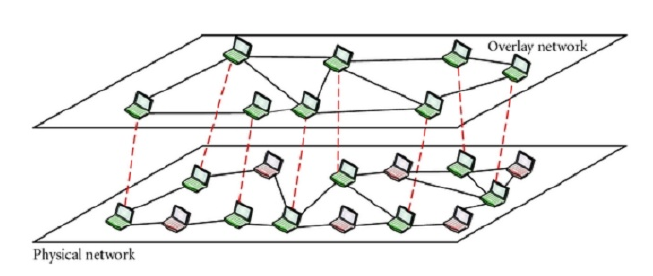
\includegraphics[scale=0.50]{img/over.png}
			\caption{Overlay network}
		\end{figure}
		La struttura del sistema è trasparente all'utente:
		\begin{itemize}
			\item Un utente non sa dire dove la computazione ha avuto luogo;
			\item La posizione dei dati è indifferente.
		\end{itemize}
		Risulta molto difficile ottenere davvero questo tipo di trasparenza nei confronti dell'utente: i sistemi distribuiti sono complessi e composti da molti elementi che possono fallire in qualsiasi momento. Vediamo quali sono le tipologie di trasparenza che si possono ottenere:
	\subsubsection{Obiettivi di un sistema distribuito}
		\textbf{Il primo obiettivo} che trattiamo è la condivisione delle risorse: deve essere facile per l'utente accedere alle risorse remote che si tratti di dispositivi, potenza computazionale, files o dati.\\
		\textbf{Il secondo} riguarda la \textbf{trasparenza} ovvero dare all'utente un'interfaccia uniforme che nasconda la natura distribuita del sistema in modo tale che quest'ultimo sia percepito come un singolo computer system. Esistono diversi tipi di trasparenza:
		\begin{itemize}
			\item \textbf{Access trasparency}: ha a che fare con diverse rappresentazioni dei dati nel sistema distribuito. L'obiettivo è trovare un accordo su come i dati sono presentati in modo tale che questi possano essere acceduti da sistemi diversi (differenti OS, JSON è una soluzione).
			\item \textbf{Location transparency}: nascondere all'utente dove la risorsa richiesta è collocata fisicamente. Si utilizzano \textbf{nomi logici}, indipendenti dalla locazione della risorsa (es URL).
			\item \textbf{Migration transparency}: nascondere il fatto che una risorsa può essere spostata fisicamente (fare in modo che la modalità di accesso cambi in relazione alla posizione fisica della risorsa);
			\item \textbf{Relocation transparency}: nasconde il fatto che una risorsa può essere spostata fisicamente in un altra posizione del sistema \textbf{mentre è utilizzata}.
			\item \textbf{Replication transparency}: replicare le risorse su più macchine è fondamentale in un sistema distribuito. La relativa trasparenza è volta a nascondere il fatto che esistano diverse copie della risorsa nel sistema. Sono necessari \textbf{nomi logici} e \textbf{trasparenza locale} (\textbf{problema di consistenza tra copie}).
			\item \textbf{Concurrency transparency}: nascondere più utenti possano accedere alla stessa risorsa lasciandola, allo stesso tempo, in uno stato consistente.
			\item \textbf{Failure transparency}: nascondere il fallimento di un nodo del sistema (es reindirizzando l'utente su un altro server).
		\end{itemize}
		Ottenere la trasparenza è difficile: le comunicazioni sono affette dal problema del delay di consegna dei messaggi, i nodi possono fallire e determinarne il fallimento è un processo lento. Inoltre dal punto di vista delle performance conservare più copie dei dati può essere molto costoso. \textbf{Dobbiamo trovare un compromesso in relazione ai requirements del sistema.}\\
		Il \textbf{terzo obiettivo è l'openess}.
		Un sistema è \textbf{aperto} se offre componenti che possono cooperare ed essere integrate in altri sistemi e se nuove risorse possono essere dinamicamente aggiunte al sistema. Le risorse sono offerte tramite i protocolli standard. Requisiti della openess: 
		\begin{itemize}
			\item \textbf{Standard interfaces}:  definisce la sinstassi e la semantica dei servizi che ogni componente offre.
			\item \textbf{Interoperabilità}: du componenti forniti da due produttori diversi possono cooperare affidandosi semplicemente alle loro interfacce.
			\item \textbf{Portabilità:} un componente sviluppato per un sistema A può essere eseguito su un sistema differente.
			\item \textbf{Estendibilità}: facile aggiungere nuovi componenti o sostituirne di vecchi senza influire sul funzionamento del sistema.
		\end{itemize}
		Per \textbf{definire le interfacce } si utilizzano gli \textbf{IDL: interface definition language} (definire nomi di funzioni, tipo dei parametri, eccezioni possibili)
		\begin{figure}[h!]
			\centering
			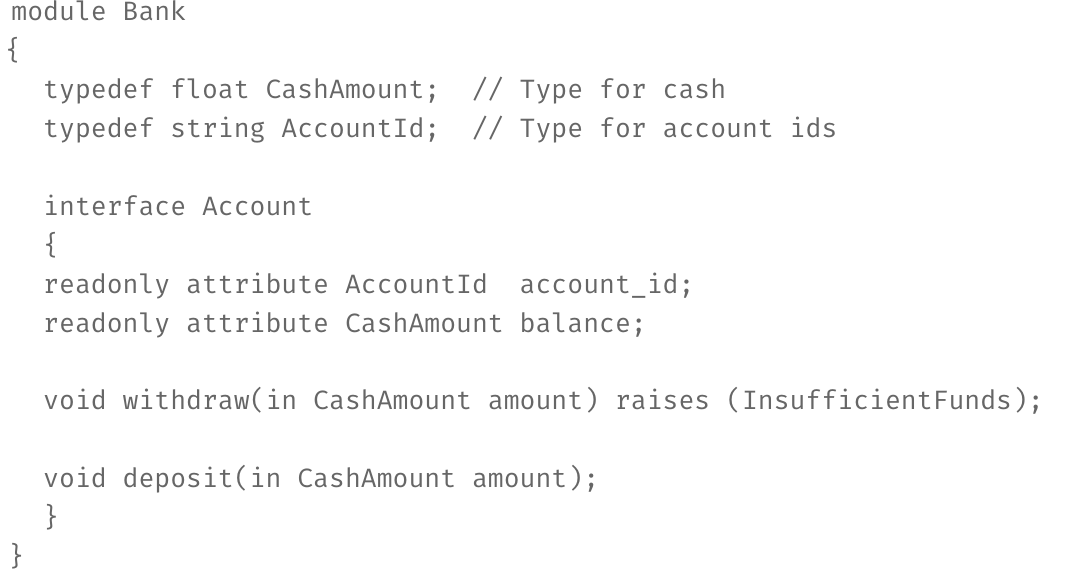
\includegraphics[scale=0.30]{img/idl0.png}
			\caption{Esempio di interfacci (IDL CORBA)}
		\end{figure}
		\textbf{Un sistema aperto è anche flessibile}: per esserlo deve essere costituito da componenti piccole e facilmente sostituibili. I sistemi tradizionali \textbf{monolitici} tendono a non esserlo. Un metodo efficace per ottenere flessibilità è quello di \textbf{dividere le politiche dai meccanismi}:
		\begin{itemize}
			\item  le \textbf{politiche} specificano cosa deve essere fatto;
			\item i \textbf{meccanismi} come deve essere fatto. 
		\end{itemize}
		L'idea è quella di modificare una politica con lo scopo di rendere più efficiente il sistema, senza intaccare i meccanismi che implementano quella politica (cambiare la priorità di schedulazione dei processi piuttosto che l'algoritmo di scheduling)\\
		\textbf{Il quarto obiettivo è la scalabilità}: la capacità del sistema di crescere e gestire carichi di lavoro sempre maggiori (tipologie in figura).
		\begin{figure}[h!]
			\centering
			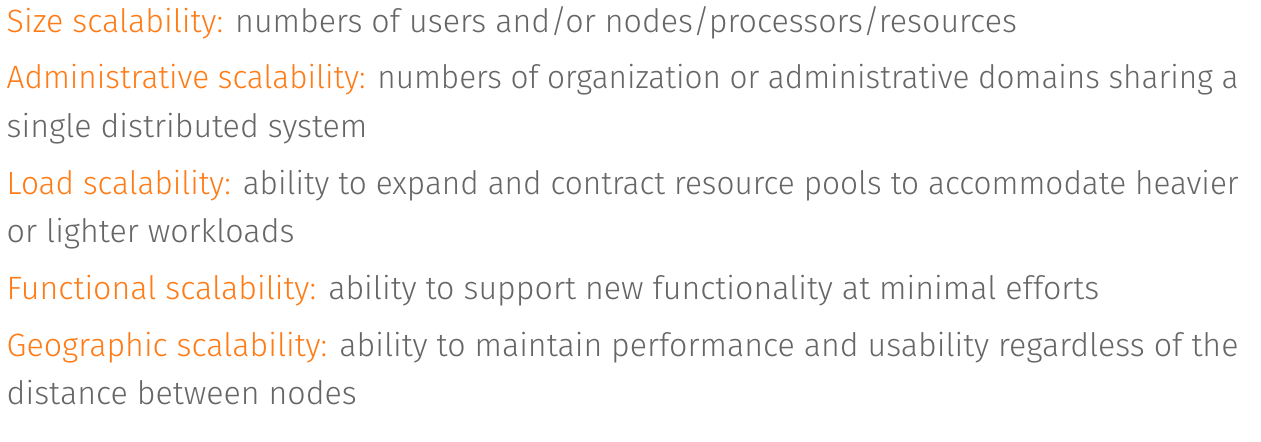
\includegraphics[scale=0.30]{img/scalab.png}
			\caption{Tipi di scalabilità}
		\end{figure}
		\begin{figure}[h!]
			\centering
			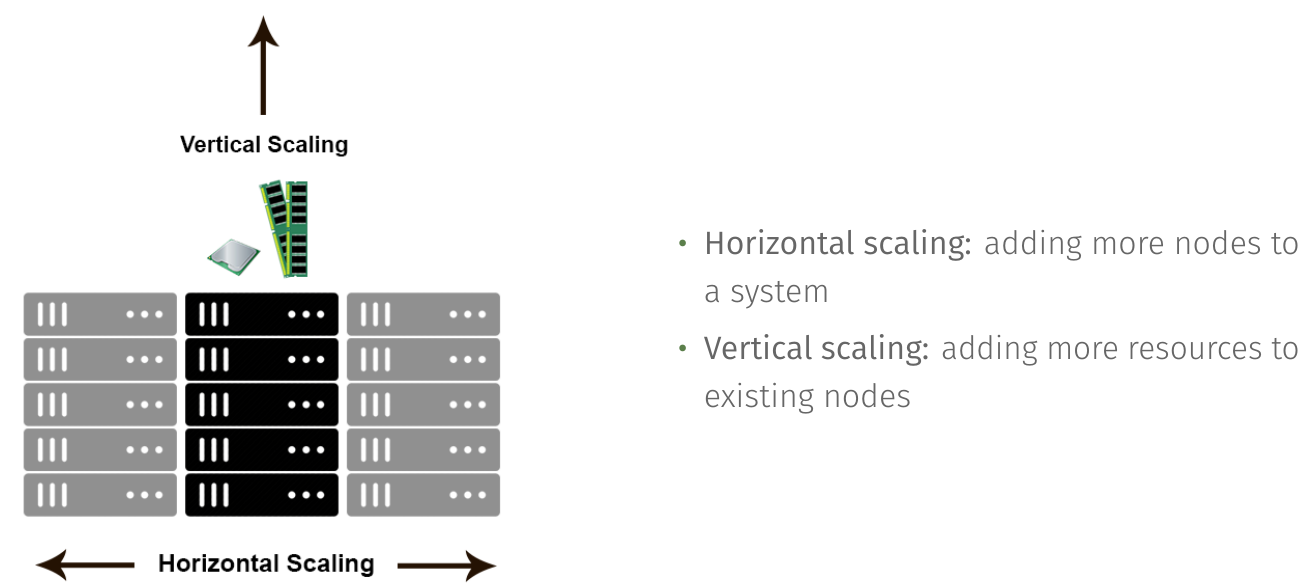
\includegraphics[scale=0.30]{img/scalab1.png}
			\caption{Tipi di scalabilità}
		\end{figure}
	\subsubsection{Nascondere le latenze di comunicazione}
		Nascondere quanto più possibile la latenza di comunicazione è fondamentale in un sistema distribuito. Nel concreto vogliamo che l'utente non attenda nell'utilizzo di un servizio remoto. In generale esistono due tipologie di comunicazione:
		\begin{itemize}
			\item \textbf{Sincrone}: il mittente interrompe l'esecuzione finchè il destinatario non riceve il messaggio;
			\item \textbf{Asincrone}: il mittente invia il messaggio e continua con la propria esecuzione.
		\end{itemize}
		\begin{figure}[h!]
			\centering
			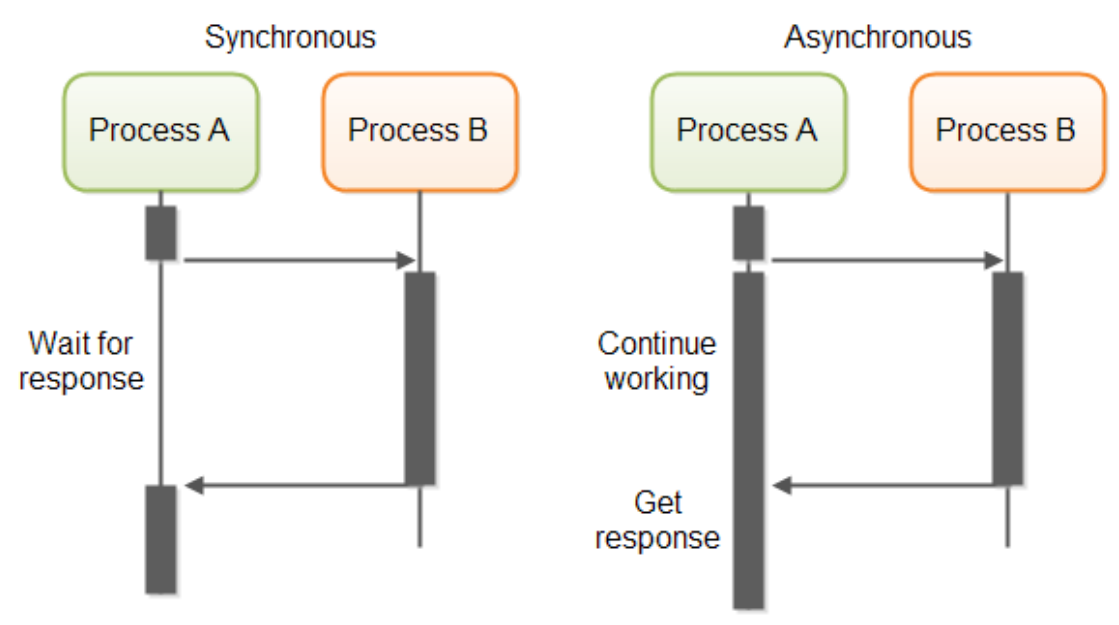
\includegraphics[scale=0.30]{img/assy.png}
			\caption{Asincrono vs sincrono}
		\end{figure}
		Un'idea per risolvere il problema potrebbe essere quella di \textbf{spostare la computazione sul cliente} (vedi figura)
			\begin{figure}[h!]
			\centering
			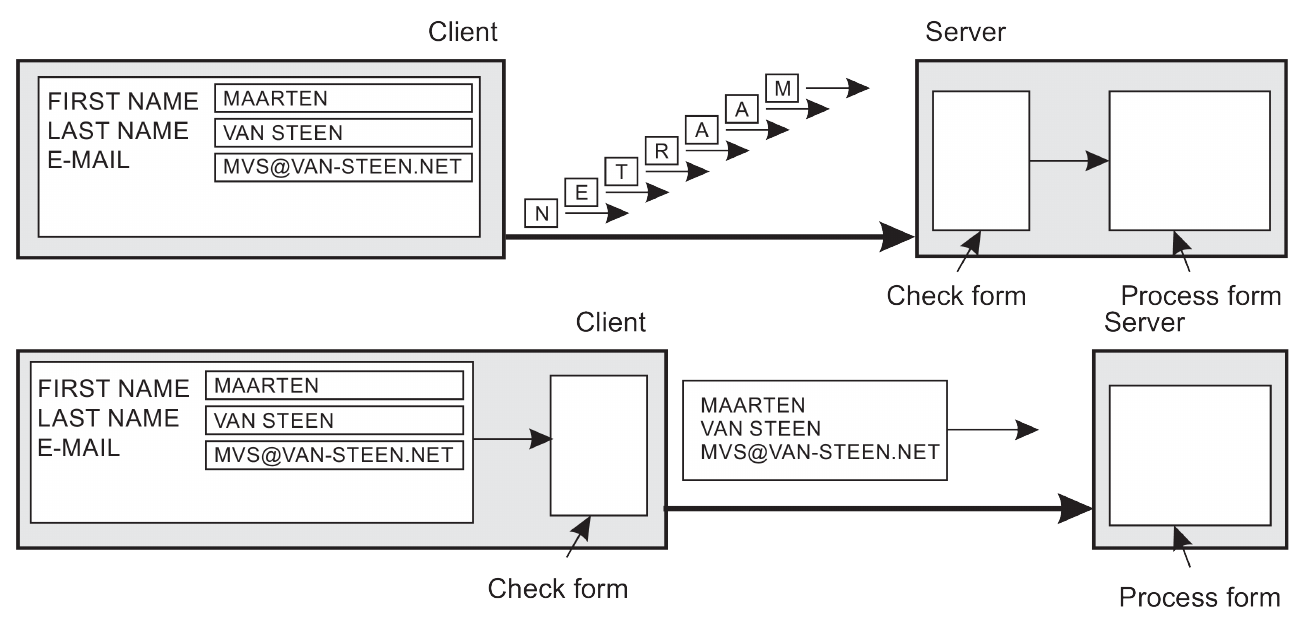
\includegraphics[scale=0.30]{img/move.png}
			\caption{Spostare la computazione sul client}
		\end{figure}
		\textbf{Il caching } è un'altra possibile soluzione (avere più copie di una risorsa posizionate in piu componenti del sistema).\\
		In istanza finale, quello che vogliamo ottenere sono:
		\begin{itemize}
			\item \textbf{Availability}: ogni richiesta fatta il sistema si deve tradurre in una risposta. Ciò implica una pronta reazione ai fallimenti e la capacità di ripristinare il sistema in seguito ad uno di essi.
			\item \textbf{Modularity}: il sistema deve essere composto da piccole parti.
		\end{itemize}
		\begin{figure}[h!]
			\centering
			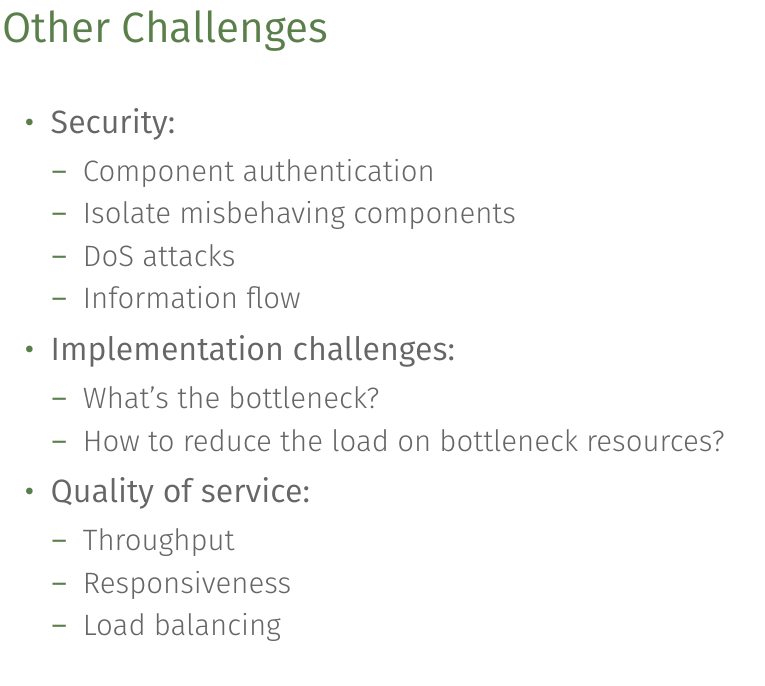
\includegraphics[scale=0.30]{img/other.png}
			\caption{Altre sfide nella modellazione di un sistema distribuito}
		\end{figure}
	
	\subsubsection{Java socket}
		Le socket sono \textbf{endpoint} di un canale di comunicazione bidirezionale tra due host:
		\begin{itemize}
			\item un endpoint è una coppia indirizzo IP e numero di porta, quindi una socket associata ad un IP e una porta.
			\item una connessione TCP è identificata da due endpoint
		\end{itemize}
		\begin{figure}[h!]
			\centering
			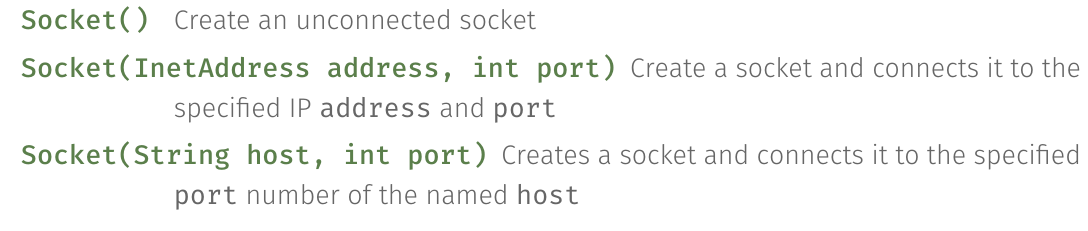
\includegraphics[scale=0.30]{img/soc.png}
			\caption{Metodi java socket}
		\end{figure}
		\begin{figure}[h!]
			\centering
			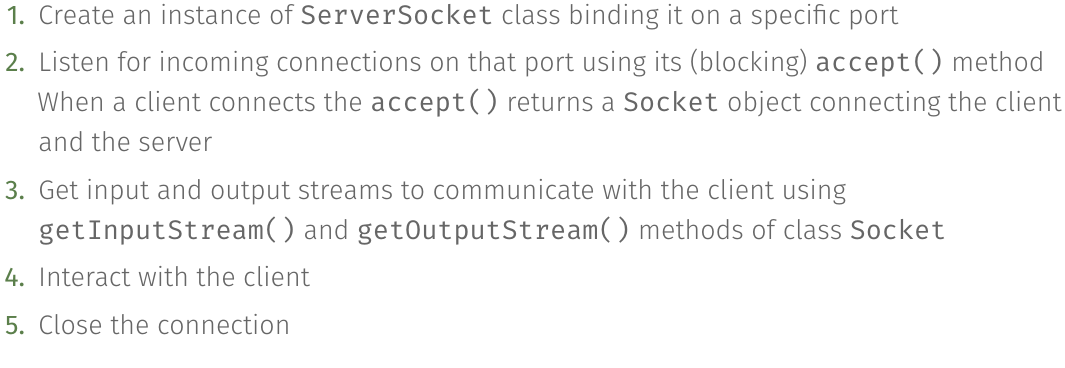
\includegraphics[scale=0.30]{img/echo.png}
			\caption{Passi per creare un server con java socket}
		\end{figure}
		
\section{Sistemi Distribuiti }
	\subsection{Architetture}
	Esistono due livelli attraverso i quali studiare l'organizzazione di un sistema:
	\begin{itemize}
		\item \textbf{Architettura Software} (organizzazione logica): definisce quali sono le componenti del sistema, quali sono i paradigmi di comunicazione, i ruoli e le responsabilità di ogni componente.
		\item \textbf{Architettura di sistema} (organizzazione fisica); 
	\end{itemize}
	\subsubsection{Architetture software: layered architecture}
		Le componenti sono organizzate in livelli. Un componente al livello i può fare una chiamata ai livelli sottostanti j. Una componente i può fare una chiamata ai livelli superiori per \textbf{notificare l'occorrenza di un evento}.
		\begin{figure}[h!]
			\centering
			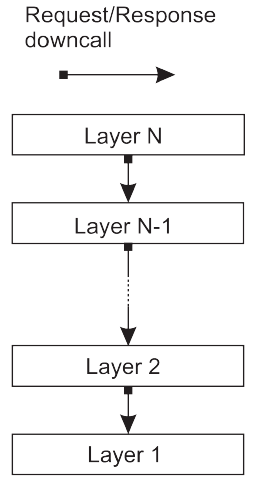
\includegraphics[scale=0.30]{img/boh.png}
			\caption{Layered architecture}
		\end{figure}
	 Un esempio è la pila ISO/OSI. Un altro esempio è quello generico dell'application layer che è strutturato in 3 livelli:
	 \begin{itemize}
	 	\item \textbf{Presentation layer}: gestisce le interazioni con gli utenti ;
	 	\item \textbf{Processing Layer}: svolge i calcoli e gestisce l'applicazione;
	 	\item \textbf{Data Layer}: gestisce il salvataggio dei dati.
	 \end{itemize}
 	\subsubsection{Architetture software: Object-based architecture }
 		Le \textbf{componenti sono oggetti} che interagiscono attraverso chiamate di metodo. Gli oggetti sono distribuiti su macchine differenti pertanto dobbiamo implementare delle chiamate remote. \textbf{Gli oggetti sono dotati di un'interfaccia e di uno stato} (facilmente sostituibili con oggetti con la stessa interfaccia). Vediamo l'architettura in dettaglio:
 		\begin{figure}[h!]
 			\centering
 			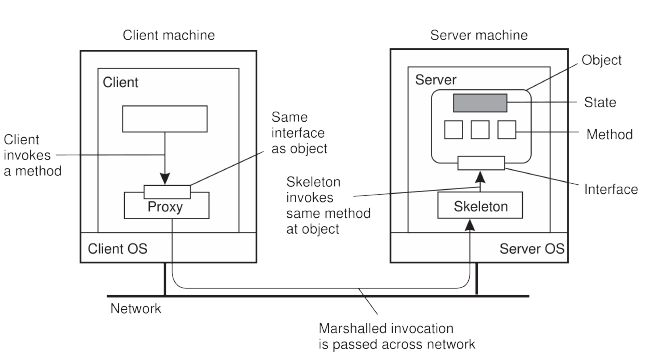
\includegraphics[scale=0.40]{img/oba.png}
 			\caption{Layered architecture}
 		\end{figure}
 		\begin{itemize}
 			\item L'oggetto è sul server;
 			\item Il proxy implementa l'interfaccia dell'oggetto e resta sul client. Svolge il compito di eseguire il marshaling dei parametri necessari all'invocazione del metodo e di eseguire l'unmarshaling delle risposte contenenti i risultati;
 			\item lo scheletro riceve la richiesta di invocazione, esegue l'unmarshaling dei parametri ed esegue la chiamata a metodo. (esempio java rmi).
 		\end{itemize}
 	\subsubsection{Architetture software: Service oriented}
 		Le componenti sono \textbf{servizi} che interagiscono attraverso i protocolli di rete. I servizi possono essere implementati da provider diversi utilizzando tecnologie diverse. Da questo punto di vista un'applicazione distribuita è una composizione di servizi che cooperano in armonia. Vediamo gli attori principali in questa architettura:
 		\begin{figure}[h!]
 			\centering
 			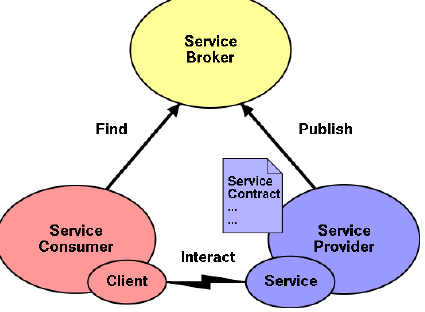
\includegraphics[scale=0.40]{img/boh1.png}
 			\caption{Layered architecture}
 		\end{figure}
 		\begin{itemize}
 			\item \textbf{Broker}: ha le informazioni su quali sono i servizi disponibili per gli utenti;
 			\item \textbf{Provider}: fornisce il servizio e fornisce al broker le informazioni su quest'ultimo.
 			\item \textbf{Consumer}: consulta il broker per sapere quali sono i servizi disponibili. Successivamente richiede al provider il servizio scelto.
 		\end{itemize}
 		Un altro concetto importante in questo tipo di architettura è quello di \textbf{orchestration}. All'interno del sistema è presente un \textbf{orchestratore} che gestisce l'interazione tra i servizi differenti
 		\begin{figure}[h!]
 			\centering
 			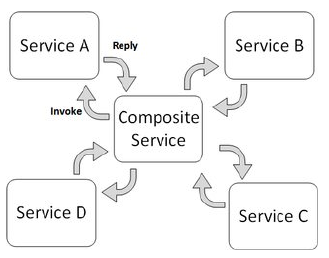
\includegraphics[scale=0.40]{img/orch.png}
 			\caption{Layered architecture}
 		\end{figure}
 	\subsubsection{Restful architecture}
 		In questo tipo di architettura un sistema distribuito è una \textbf{collezione di risorse}. Vediamo le 4 caratteristiche principali
 		\begin{itemize}
 			\item Ogni risorsa viene identificata da un URI;
 			\item Ogni servizio offre le stesso 4 operazioni
 			\item esecuzione \textbf{stateless}
 			\item Ogni messaggio è completamente auto descrittivo ( contiene tutte le informazioni necessarie per processarne il contenuto).
 		\end{itemize}
 		\begin{figure}[h!]
 			\centering
 			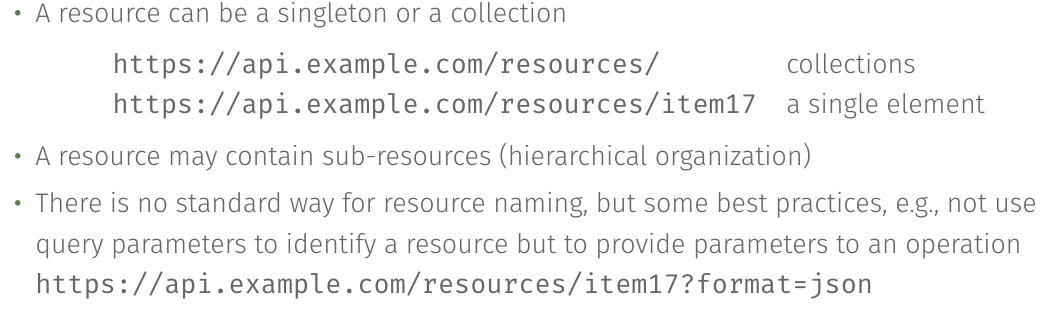
\includegraphics[scale=0.40]{img/rest.png}
 			\caption{Risorse rest}
 		\end{figure}
 		\begin{figure}[h!]
 			\centering
 			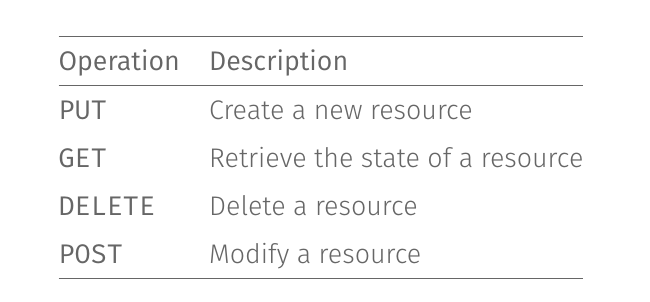
\includegraphics[scale=0.40]{img/rest1.png}
 			\caption{Operazioni rest}
 		\end{figure}
 		Da notare che questa architettura è:
 		\begin{itemize}
 			\item \textbf{Referentially coupled}: durante la comunicazione le componenti utilizzano riferimenti diretti al proprio partner di comunicazione.
 			\item \textbf{Temporally coupoled}: per comunicare le componenti devono essere in esecuzione.
 		\end{itemize}
 	\subsubsection{Publish subscribe architecture}
 	 Ha tre tipi di componenti:
 	 \begin{itemize}
 	 	\item \textbf{Publisher}: invia messaggi in broadcast senza sapere se verrano ricevuti;
 	 	\item \textbf{subscriers}: sta in ascolto per i messaggi che gli interessi e non ha nessuna conoscenza riguardo al publisher.
 	 	\item \textbf{Broker}: intermediario tra i due.
 	 \end{itemize}
  	Il sistema è aperto, ciò significa che non c'è un limite al numero di sub e pub, tuttavia il broker rappresenta il collo di bottiglia del protocollo.\\
  	\begin{figure}[h!]
  		\centering
  		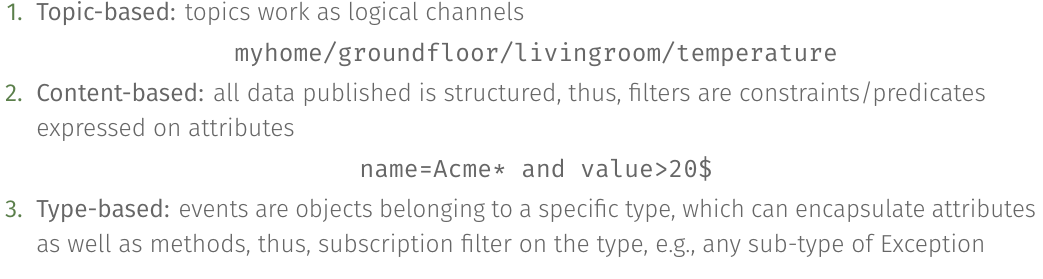
\includegraphics[scale=0.40]{img/bi.png}
  		\caption{Tipi di messaggi}
  	\end{figure}
 	Un \textbf{evento} consiste alla presenza di un nuovo dato disponibile. In questo caso il sistema può inoltrare la notifica insieme al dato oppure inoltrare solo la prima.
 	Ricordiamo che il modello è :
 	\begin{itemize}
 		\item \textbf{referentially decoupled}: le componenti non devono conoscersi per comunicare.
 		\item \textbf{Temporally decoupled}: non devono essere entrambe attive per comunicare.
 	\end{itemize}
 	\subsubsection{Tuple space architecture}
 		Le componenti comunicano tra di loro attraverso tuple che vengon salvate all'interno del tuple space (spazio condiviso).
 		\begin{itemize}
 			\item le componenti salvano tuple all'interno del tuple- space.
 			\item per recuperare un tupla una componente deve fornire un pattern di ricerca che coincida con la tupla (in(array,primes,int,int))
 			\item il tuple space è persistente: le tuple non vengono rimosse se non esplicitamente.
 			\item produttore e consumatore non devono esistere nello stesso momento.
 		\end{itemize}
 	\subsubsection{Architetture di sistema: client/server }
 	 	
 		\begin{figure}[h!]
 			\centering
 			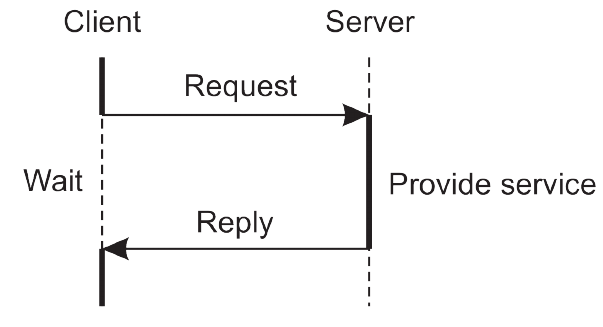
\includegraphics[scale=0.40]{img/clie.png}
 			\caption{Architettura client server}
 		\end{figure}
 		Questa architettura utilizza NFS come modello di accesso remoto ai file:
 		\begin{itemize}
 			\item al client è offerto accesso trasparente al file system gestito dal server
 			\item Le operazioni offerte al client sono implementate sul server.
 			\item ogni operazione su un file richiede la comunicazione con il server
 		\end{itemize}
 		In alternativa possiamo utilizzare un modello \textbf{upload/download}:
 		il client scarica il file, esegue le operazioni ed esegue l'upload del file sul server quando ha terminato. Vediamo alcune organizzazioni tipiche:
 		\begin{itemize}
 			\item \textbf{Single tier}: l'applicazione è sul server, il terminale permette solo di accedere al mainframe.
 			\item \textbf{Two-tier}: il primo strato si trova sul client, il secondo sul server 
 			\item \textbf{Three-tier}: ogni layer è su una macchina diversa.
 		\end{itemize}
 		\begin{figure}[h!]
 			\centering
 			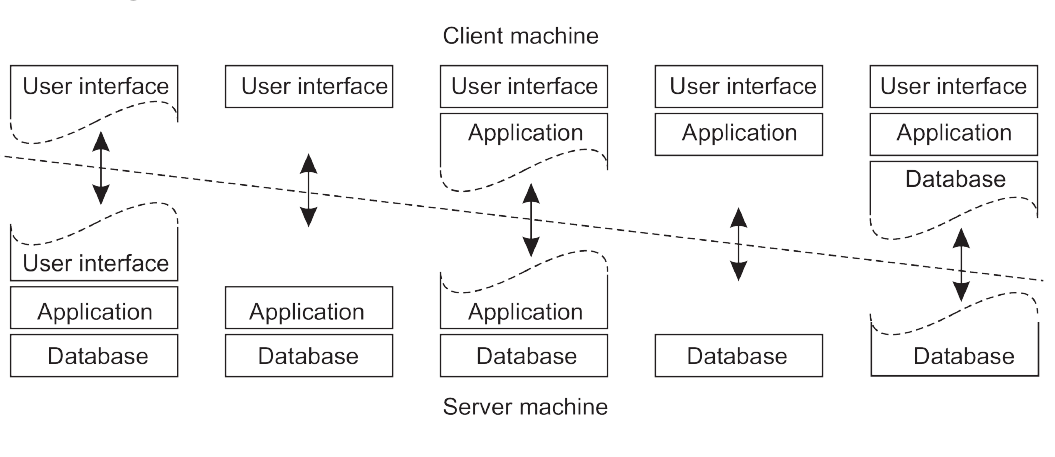
\includegraphics[scale=0.40]{img/two.png}
 			\caption{two tier}
 		\end{figure}
 		\begin{figure}[h!]
 			\centering
 			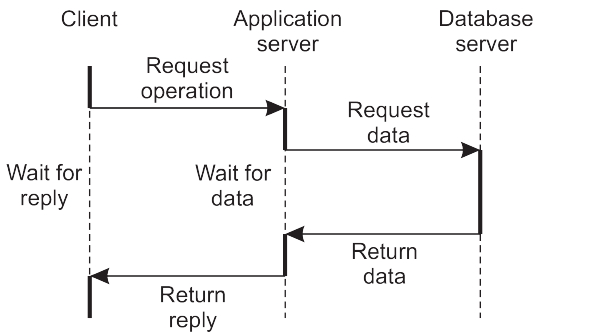
\includegraphics[scale=0.40]{img/three.png}
 			\caption{three tier}
 		\end{figure}
 	\subsubsection{Architettura peer to peer}
 		In questo tipo di architettura non abbia nessuna distinzione tra client e server: ogni nodo partecipa al sistema condividendo le proprie risorse. L'obiettivo è quello di condividere risorse di un gran numero di partecipanti con lo scopo di svolgere un compito. I \textbf{peer} eseguono lo stesso programma e forniscono la stessa interfaccia. L'interazione è dunque \textbf{simmetrica}
 		\begin{figure}[h!]
 			\centering
 			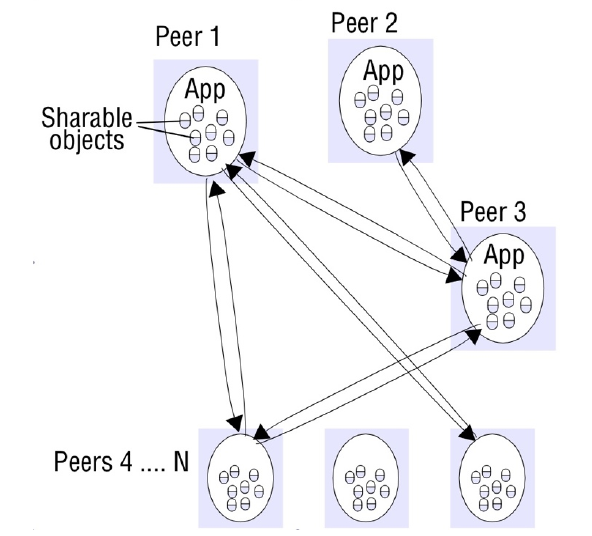
\includegraphics[scale=0.40]{img/p2p.png}
 			\caption{p2p architecture}
 		\end{figure}
 	\subsubsection{P2P overlay network non strutturata}
 	\begin{itemize}
 		\item ogni peer mantiene un lista locale di peer, quando un peer si unisce alla rete prima contatta uno di questi peer per farsi dare la lista dei partecipanti correnti al sistema.
 		\item il peer scegli una partizione di peer a cui connettersi
 		\item la topologia della rete risultante è quella di un grafo casuale ovvero un grafo in cui un arco esiste solo con una certa probabilità. 
 	\end{itemize}
 	Le \textbf{risorse} sono distribuite nei peer che partecipano al sistema: cercare una risorsa significa cercare i peers che sono responsabili per tale risorsa. Un peer conosce solo la sua lista dei peer locali e le risorse per cui essi sono responsabili. \textbf{Come può un peer individuare le risorse che gli servono?}
 	In un overlay network non strutturata si hanno due strategie possibili:
 	\begin{itemize}
 		\item \textbf{Floodind}: un peer passa la richiesta per una risorsa a tutti i suoi vicini. Un vicino può fornire la risorsa se la possiede altrimenti inoltra la query a tutti i suoi vicini.
 		\item \textbf{Random Walk} stesso procedimento ma casuale.
 	\end{itemize}
 	\subsubsection{P2P overlay network strutturata}
 		La rete ha una specifica topologia (anello, albero). Ogni risorsa del sistema è associata ad una chiave, dunque il sistema salva  coppie \textbf{(chiave,valore)} (DHT)
 		
 \subsection{Jersey}
	Jersey è un framework per costruire \textbf{servizi web REST} (implementa le API \textbf{JAX-RS}).
	JAX-RS implementa API Java per i servizi REST ovvero una serie di annotazioni, classi e interfacce che possono essere utilizzate per esporre risorse POJO (assume http come protocollo di comunicazione sottostante). 
	\begin{figure}[h!]
		\centering
		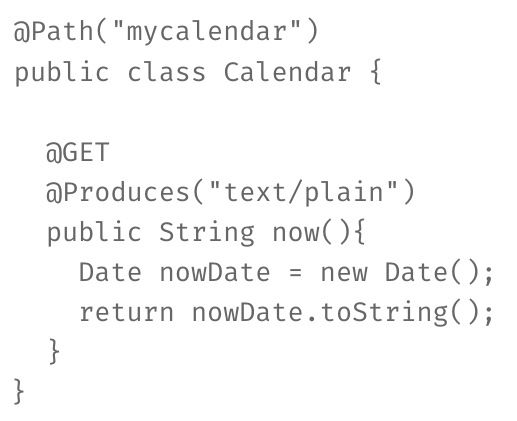
\includegraphics[scale=0.40]{img/pojo.png}
		\caption{p2p architecture}
	\end{figure}
	Concetti fondamentali:
	\begin{itemize}
		\item \textbf{Resource class}: classe Java che utilizza annotazioni JS-RX
		\item \textbf{Root resource class}: una classe di risorse annotata con @path
		\item \textbf{Request method deignator}: annotazione Java utilizzata per identificare un oggetto HTTP
		\item \textbf{Resource method}: un metododo di una risorsa annotato con un request method designator  
	\end{itemize}
	\begin{figure}[h!]
		\centering
		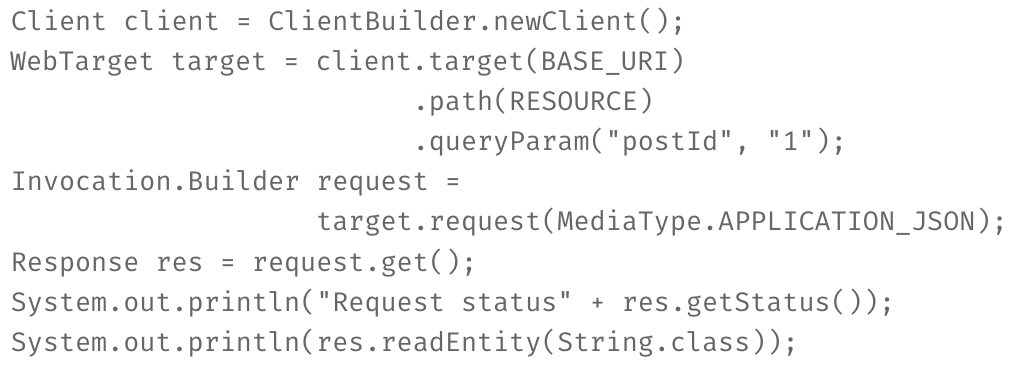
\includegraphics[scale=0.40]{img/invoc.png}
		\caption{Esempio invocazione}
	\end{figure}
	WebTarget è un costrutto che ci permette di definire una richiesta per una specifica risorsa, ne otteniamo così l'URI relativo e possiamo inoltre passare dei parametri per un'eventuale query avanzata.
	\textbf{InvocationBuilder} usa la richiesta formata attraverso WebTarget generando una richiesta http.
	\begin{figure}[h!]
		\centering
		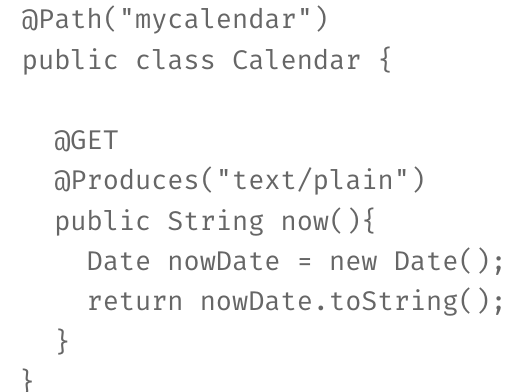
\includegraphics[scale=0.40]{img/rest2.png}
		\caption{Annotazioni rest}
	\end{figure} 
	\begin{figure}[h!]
		\centering
		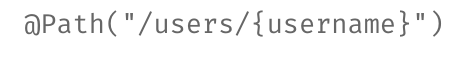
\includegraphics[scale=0.40]{img/pat.png}
		\caption{@path}
	\end{figure} 
	\begin{figure}[h!]
		\centering
		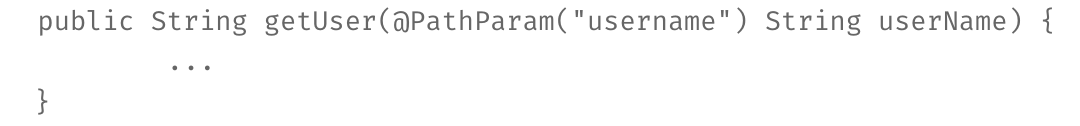
\includegraphics[scale=0.40]{img/pat1.png}
		\caption{@path}
	\end{figure} 
	\begin{itemize}
		\item \textbf{@path}: annotazione utilizzata per definire dove la classe ha il suo path di origine. \textbf{@pathparam} è utilizzata nei parametri del metodo per indicare che quel parametro serve ad indicare una particolare risorsa nel path.  
		\item \textbf{@GET, @PUT, @POST, @DELETE}: utilizzate per annotare i metodi
		\item \textbf{@Produces}: si utilizza per indicare che tipo di risorsa verrà prodotta per il client.
		\item \textbf{@Consumes}: associato ad un metodo @POST definisce il tipo dei parametri della richiesta.
	\end{itemize}
	\begin{figure}[h!]
		\centering
		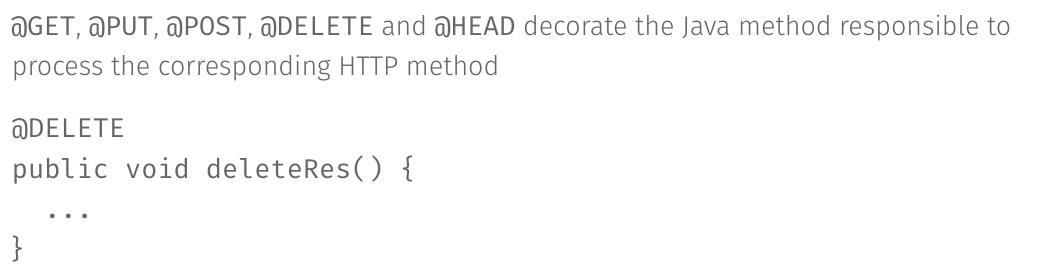
\includegraphics[scale=0.40]{img/annotation.png}
		\caption{Annotazioni}
	\end{figure} 
	\begin{figure}[h!]
		\centering
		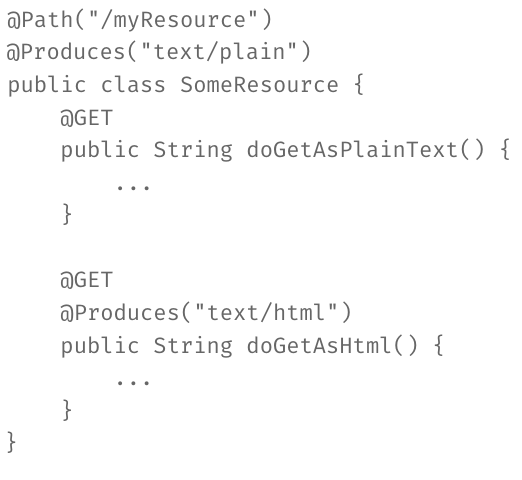
\includegraphics[scale=0.40]{img/annotation1.png}
		\caption{Annotazioni}
	\end{figure} 

	   
 	
 		
 		
 		
 		
 		
 		
		
		
		
		
		
		
	
\section{Communication Mechanisms}
	\subsection{Middleware}	
		\begin{figure}[h!]
			\centering
			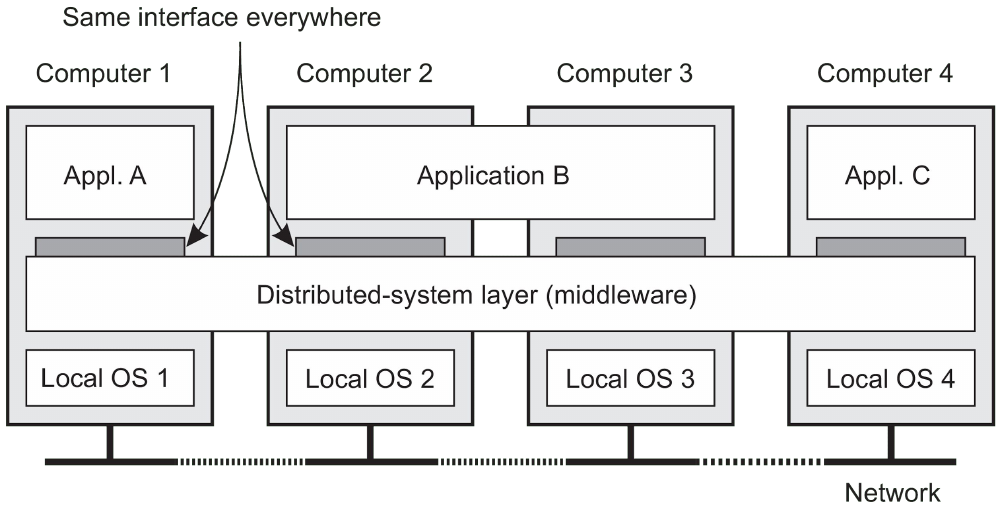
\includegraphics[scale=0.50]{img/middle.png}
			\caption{Livello Middleware}
		\end{figure}
		Il \textbf{middleware} è un insieme di applicazioni e protocolli "\textbf{general purpose}" che risiedono all'interno del livello applicativo. è dunque un livello software che astrae dall'eterogeneità di rete, hardware, sistemi operativi e linguaggi di programmazione, con lo \textbf{scopo di fornire interfacce comuni che assicurino  modelli di comunicazione e di computazione uniformi}.  Questo livello, dunque, costituisce un insieme di protocolli condivisi dalle applicazioni più specifiche al livello soprastante.
		In sintesi, un livello middleware offre servizi alle applicazioni quali:
		\begin{itemize}
			\item Comunicazione;
			\item Meccanismi di sicurezza;
			\item Transazioni
			\item Error-recovery;
			\item Gestione di risorse condivise.
		\end{itemize}
		\textbf{Questi servizi sono indipendenti rispetto alle specifiche applicazioni.} 
		Alcuni esempi:
		\begin{itemize}
			\item Protocolli di autenticazione e autorizzazione (criptografia ssh)
			\item Protocolli di commit. Sono utilizzati per realizzare l'atomicità nelle transazioni. Stabiliscono se in un insieme di processi tutti hanno svolto una particolare operazione o se non è stata svolta affatto.
		\end{itemize}
		Nello specifico vedremo come i \textbf{protocolli di comunicazione middleware supportino servizi di comunicazione ad alto livello} e permettano, per esempio, la chiamata a procedure o oggetti remoti in modo \textbf{trasparente.}
			 
	\subsection{Coordinazione diretta}	
		Un tipi di comunicazione nella quale le componenti partecipanti sono:
		\begin{itemize}
			\item \textbf{Referentially coupled}: durante la comunicazione gli attori utilizzano riferimenti espliciti ai loro interlocutori.
			\item \textbf{Temporally coupled}: entrambe le componenti devono essere in esecuzione (up and running).	
		\end{itemize}
		Il libro propone un'introduzione ai tipi di comunicazione (persist, transient, synchronous, asynchronous).
		
	\subsection{Remote Procedure Call}
		Molti sistemi distribuiti sono basati sullo scambio di messaggi tra processi, tuttavia questo tipo di approccio non permette di nascondere la comunicazione tra le componenti in modo da rendere trasparente il contesto distribuito. \\
		Una soluzione al problema è stata proposta da Nelson e Birrell (1984) introducendo una modalità completamente differente nella gestione della comunicazione nel contesto di un sistema distribuito.
		In breve la proposta è quella di chiamare procedure che sono localizzate su macchine remote:
		\begin{enumerate}
			\item quando A chiama B il processo chiamante in A è sospeso;
			\item l'esecuzione della procedura chiamata ha luogo in B;
			\item A invia i parametri della chiamata a B che a sua volta risponderà con il risultato della chiamata;
			\item \textbf{Nessun passaggio di messaggi è visibile dal punto di vista del programmatore.}
		\end{enumerate}
		La soluzione ha le seguenti problematiche:
		\begin{itemize}
			\item le procedure chiamante e chiamato si trovano su macchine diverse e non condividono lo stesso address space;
			\item la rappresentazione dei parametri e del risultato di ritorno può differire sulle macchine interessate;
			\item Le due macchine potrebbero crashare.
		\end{itemize}
		\begin{figure}[h!]
			\centering
			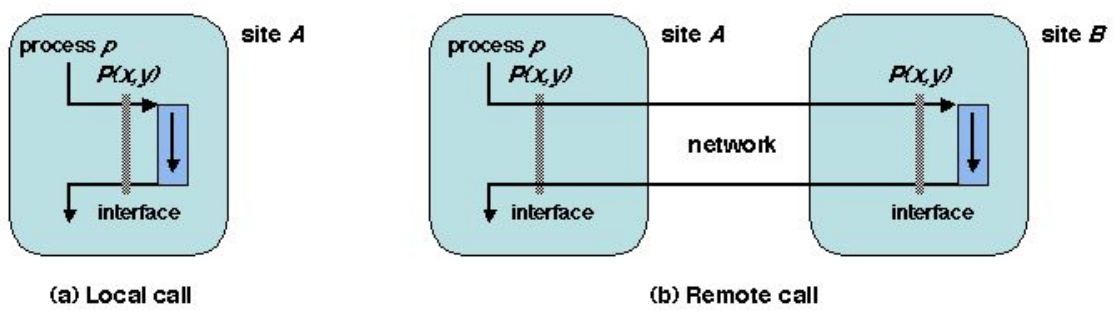
\includegraphics[scale=0.50]{img/proc.png}
			\caption{Chiamata a procedura locale vs remota}
		\end{figure}
		\begin{figure}[h!]
			\centering
			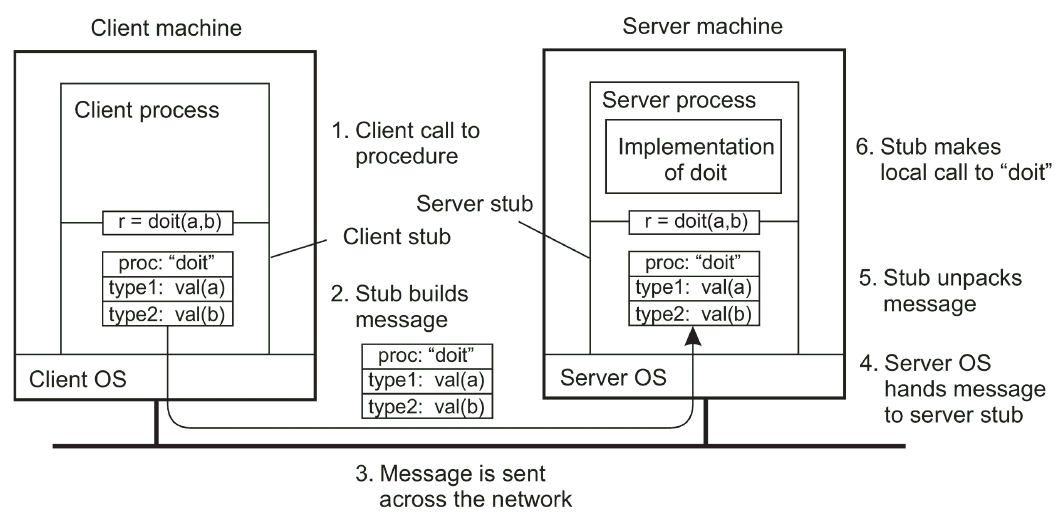
\includegraphics[scale=0.50]{img/how.png}
			\caption{Funzionamento RPC}
		\end{figure}
		Una chiamata a procedura remota deve essere \textbf{trasparente} rispetto al chiamante, per farlo viene creato uno stub locale della funzione che si trova in macchina remota. Lo stub, sia sul server che sul client implementa serializzazione e invio dei parametri e del risultato.  
		Di seguito si elencano i passi necessari ad una chiamata a procedura remota:
		\begin{enumerate}
			\item la procedura del client chiama il proprio stub;
			\item lo stub costruisce il messaggio ed effettua una chiamata al proprio OS;
			\item l'OS del client invia il messaggio all'OS remoto;
			\item l'OS remoto invia il messaggio allo stub del server;
			\item lo stub del server decomprime i parametri e chiama la procedura locale sul server;
			\item si esegue la computazione e si invia i risultati allo stub; 
			\item lo stub del server comprime i risultati e li invia al proprio OS;
			\item si invia il messaggio all'OS del client che lo passa allo stub del client;
			\item lo stub decomprime il risultato della computazione e lo passa al client
		\end{enumerate}
		
		\subsubsection{Passaggio di parametri}
			L'operazione di impacchettare parametri all'interno di un messaggio è chiamata \textbf{marhaling}, il messaggio conterrà i parametri stessi e le informazioni necessarie al destinatario. Il principale problema è il seguente: \textbf{client e server potrebbero adottare diverse rappresentazioni per i dati} (esempio diverse little endian big endian). Nel caso di utilizzo di HTTP come protocollo di trasporto il formato xml può essere utilizzato come formato comune per il passaggio dei parametri.
			\begin{figure}[h!]
				\centering
				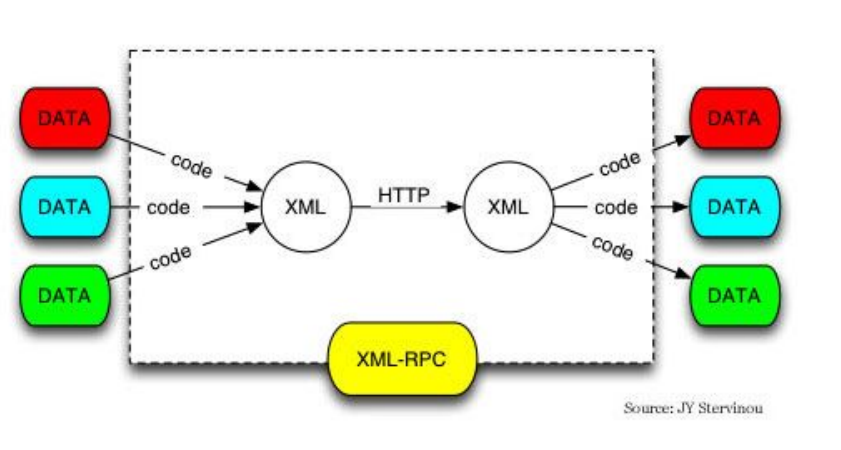
\includegraphics[scale=0.50]{img/xml.png}
				\caption{Xml }
			\end{figure}
		
			\textbf{Un problema} ulteriore risiede nel \textbf{passaggio dei puntatori e riferimenti}. Infatti, questi avranno senso solo se riferiti allo spazio di indirizzi locale del chiamante. Una possibile soluzione è quella di sostituire la \textbf{chiamata per riferimento} con un \textbf{copia/ripristina}. L'idea è quella di effettuare una copia dell'array da passare ed allegarla al messaggio destinato al server. L'array è conservato in un buffer nello stub del server ed inviato nuovamente al client una volta effettuata la chiamata remota (se richiesto). Nonostante i linguaggi offrano supporto automatico al \textbf{(un)marshaling}, quest'ultimo introduce un'\textbf{overhead} nella comunicazione, soprattutto in caso di grosse strutture dati come alberi e grafi.
			
			\begin{figure}[h!]
				\centering
				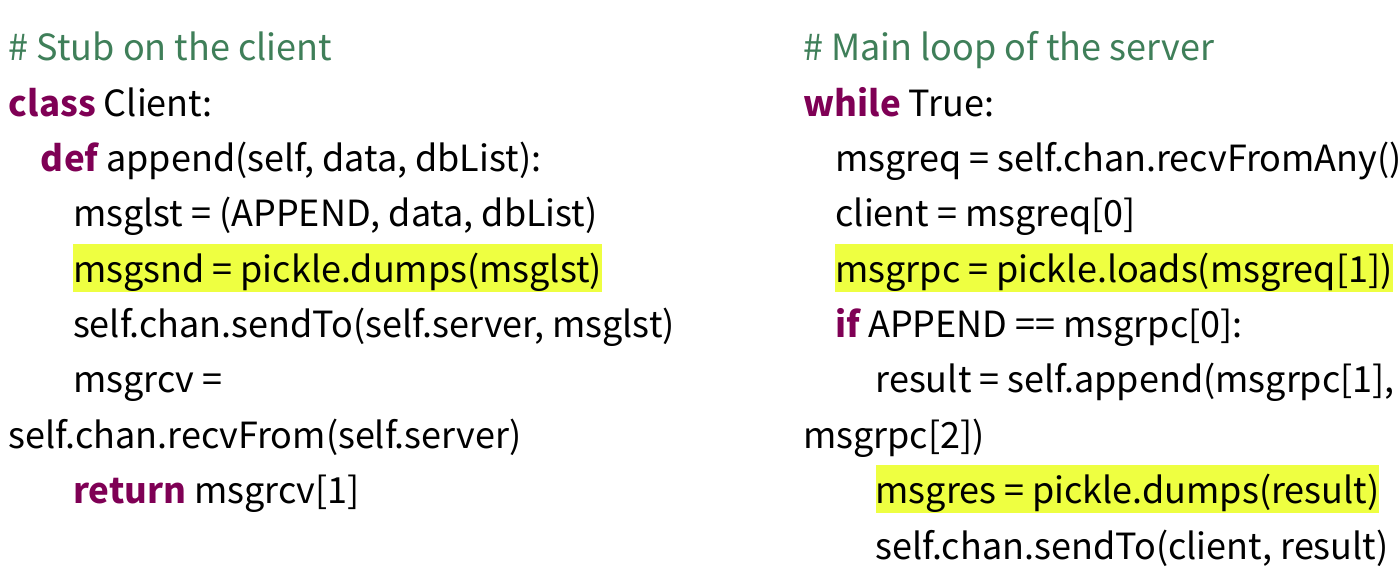
\includegraphics[scale=0.25]{img/rpccode.png}
				\caption{Marshaling in Java  }
			\end{figure}   
		
			Il problema non si presenta qualora i riferimenti siano \textbf{globali}, ovvero quando hanno un significato sia per il server sia per il client. \newline
			In generale, nel contesto di un sistema basato sugli oggetti sono definite due tipologie di oggetti:
			\begin{itemize}
				\item \textbf{Locali}: copiati e trasmessi nella loro interezza;
				\item \textbf{Remoti}: solo lo stub è copiato e trasmesso. 
			\end{itemize}
			In Java oggetti remoti o locali hanno tipi diversi (i remoti implementano l'interfaccia Remote).
			\begin{figure}[h!]
				\centering
				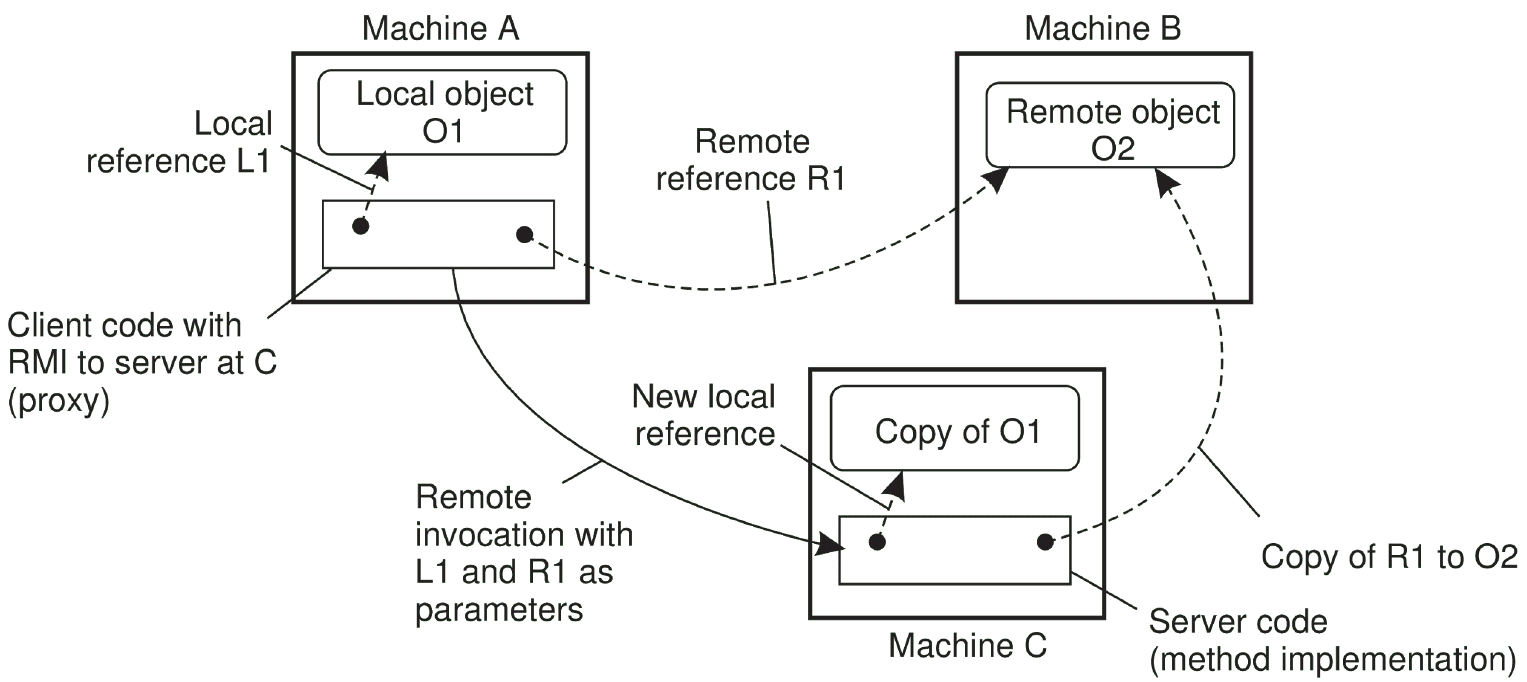
\includegraphics[scale=0.25]{img/remotelocal.png}
				\caption{Oggetti remoti e locali  }
			\end{figure}
		
		\subsubsection{Implementare RPC}
			Ci sono due modi attraverso il quale il meccanismo RPC può essere fornito allo sviluppatore:
			\begin{itemize}
				\item \textbf{Framework o libreria}: il programmatore deve specificare cosa è esportato in remoto fornendo di fatto un'\textbf{interfaccia del servizio}, che contiene tutte le procedure che possono essere chiamate dal client. I framework hanno il pregio di essere \textbf{indipendenti dal linguaggio}. Per questo è norma utilizzare un \textbf{Interface Definition Language (IDL)} che, una volta compilato, genere gli stub per client e server nel linguaggio desiderato. Di contro non abbiamo trasparenza totale per il programmatore che dunque è consapevole di trovarsi nel contesto di una chiamata a procedura remota (deve specificare egli stesso gli oggetti remoti). Alcuni esempi di framework: \textbf{Corba, GRPC, Apache Thrift}.     
				\item \textbf{Costrutti all'interno del linguaggio}: è lo stesso linguaggio a definire i costrutti necessari ad una RPC. In questo caso è il \textbf{compilatore a generare gli stub} per client e server. In questo modo si ottiene \textbf{trasparenza} per il programmatore, tuttavia client e server devono essere \textbf{implementati nello stesso linguaggio} (Es: \textbf{Java RMI}).
			\end{itemize}
		
		\subsubsection{RPC Asincrono}
			\begin{figure}[h!]
				\centering
				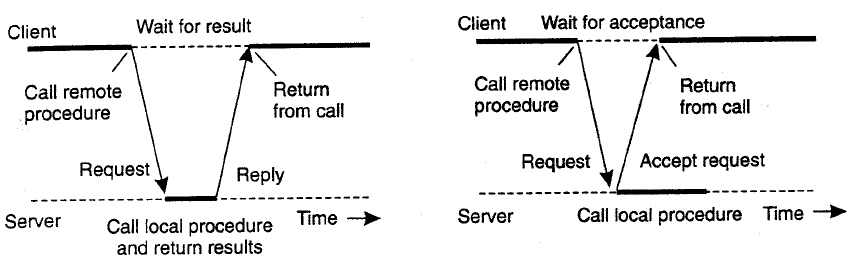
\includegraphics[scale=0.45]{img/async.png}
				\caption{RPC tradizionale e asincrona }
			\end{figure}
			A differenza del paradigma tradizionale nel quale il client attende la risposta del server bloccando la sua esecuzione, il server invia un ACK al client una volta ricevuta la richiesta. L'ACK viene inviato al client per notificare che la sua richiesta sarà processata, nel frattempo il client può eseguire ulteriori operazioni evitando di sospendere la sua esecuzione. Il Server utilizza una funzione detta di \textbf{Callback} per consegnare il risultato al Client.
			\begin{figure}[h!]
				\centering
				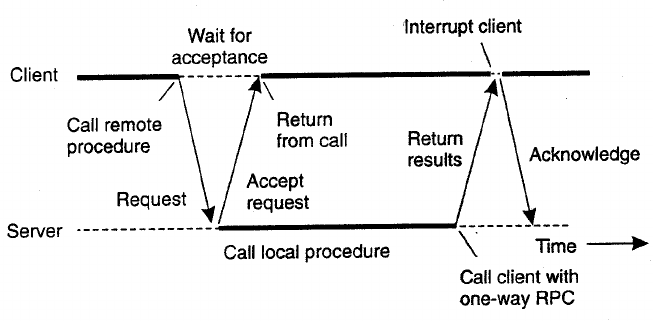
\includegraphics[scale=0.40]{img/callback.png}
				\caption{Callback }
			\end{figure}
			L'asincronicità della comunicazione permette l'implementazione di un protocollo \textbf{Multicast RPC} inviando richieste in parallelo a server diversi che dunque processano indipendentemente l'uno dall'altro. Si può definire questo protocollo nell'ottica di accettare il risultato più veloce scartando dunque gli altri, oppure per la realizzazione di una computazione distribuita, combinando i risultati ricevuti.
			
		\subsubsection{Binding}
			In applicazioni reali abbiamo bisogno di una fase preliminare chiamata \textbf{binding} che permette al client di avere un riferimento al server. Necessario per il client risulta l'utilizzo di un \textbf{registro} al cui interno sono salvate coppie (nome, indirizzo) di uno o più server. Si utilizza tale riferimento per la comunicazione.
			\begin{figure}[h!]
				\centering
				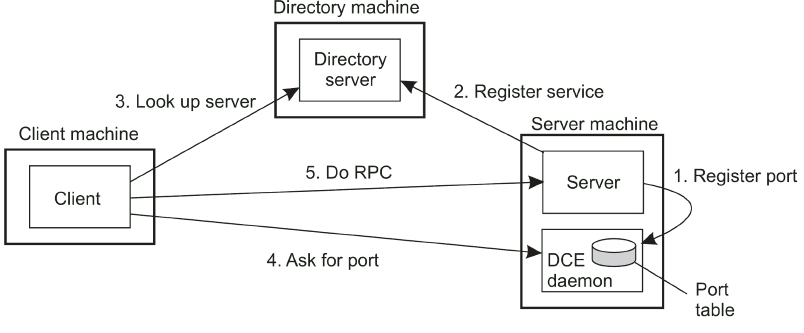
\includegraphics[scale=0.45]{img/bind.png}
				\caption{Binding }
			\end{figure}
		
	\subsection{Message Oriented Middleware}
		Questo modello di comunicazione prevede lo scambio di messaggi tra le entità partecipant. Grazie allo scambio di messaggi possiamo definire un modello nel quale, mittente e destinatario \textbf{non devono essere attivi durante lo scambio dei messaggi}. Questo è possibile grazie al Middleware che mette a disposizione buffer temporanei per i messaggi scambiati. Ogni applicazione ha a disposizione una coda locale che contiene i messaggi inviati e ricevuti e che può eventualmente essere condivisa tra più applicativi.
		\begin{figure}[h!]
			\centering
			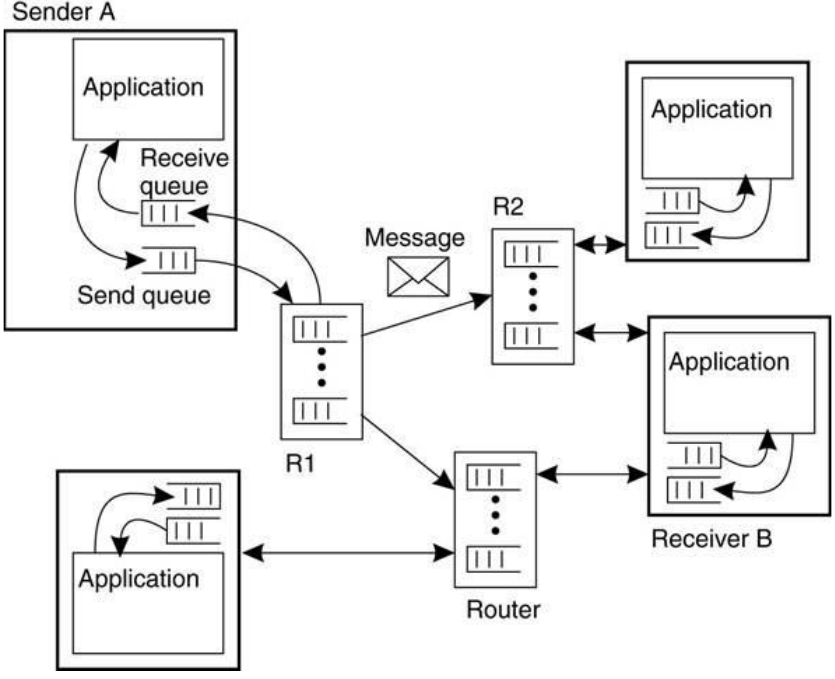
\includegraphics[scale=0.30]{img/queque.png}
			\caption{Code }
		\end{figure} 
		Il modello di comunicazione definito ha le seguenti proprietà:
		\begin{itemize}
			\item La comunicazione avviene semplicemente inserendo e rimuovendo messaggi dalla coda, un messaggio ovviamente rimane nella coda fino a che non è esplicitamente rimosso;
			\item La comunicazione è \textbf{loosely coupled}, cioò significa che il ricevente non deve essere necessariamente in esecuzione.   
		\end{itemize}
		Di seguito sono elencate le primitive concettuali che un message oriented middleware deve esporre:
		\begin{itemize}
			\item \textbf{Put}: inserisce un messaggio nella coda;
			\item \textbf{Get}: rimuove il primo messaggio dalla coda (blocking);
			\item \textbf{Poll}: rimuove il primo messaggio dalla coda (non-blocking);
			\item \textbf{Notify}: informa che un messaggio è arrivato nella coda.	
		\end{itemize}
		\newpage
		
		\subsubsection{Queue Manager}
			Il queue manager gestisce i messaggi inviati o ricevuti da un'applicazione nella sua coda (ad ogni applicazione è associata una coda e un relativo manager). Può essere implementato come una libreria collegata all'applicazione o come un \textbf{processo separato}. \textit{Nel secondo caso il sistema supporterà la comunicazione asincrona persistente}.
			\begin{figure}[h!]
				\centering
				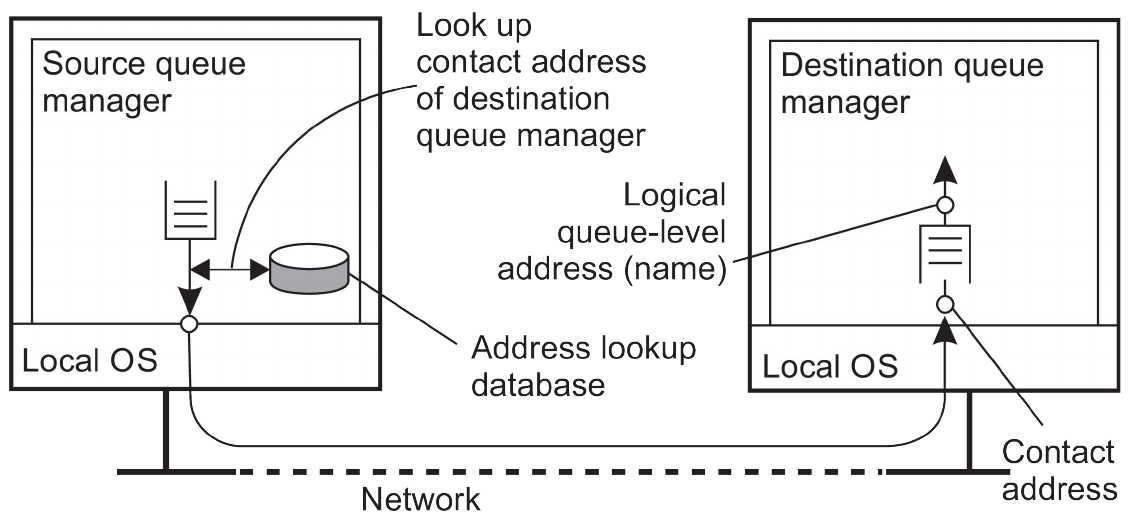
\includegraphics[scale=0.30]{img/mana.png}
				\caption{Queue Manager }
			\end{figure}
			In definitiva questi processi operano come \textbf{router} o \textbf{relay} inoltrando i messaggi ricevuti ad altri queue manager. In questo modo il sistema di quequing può costituire \textbf{un livello applicazione a se stante (Overlay network )} (un'astrazione), basato su una rete di computer esistente.
			\begin{figure}[h!]
				\centering
				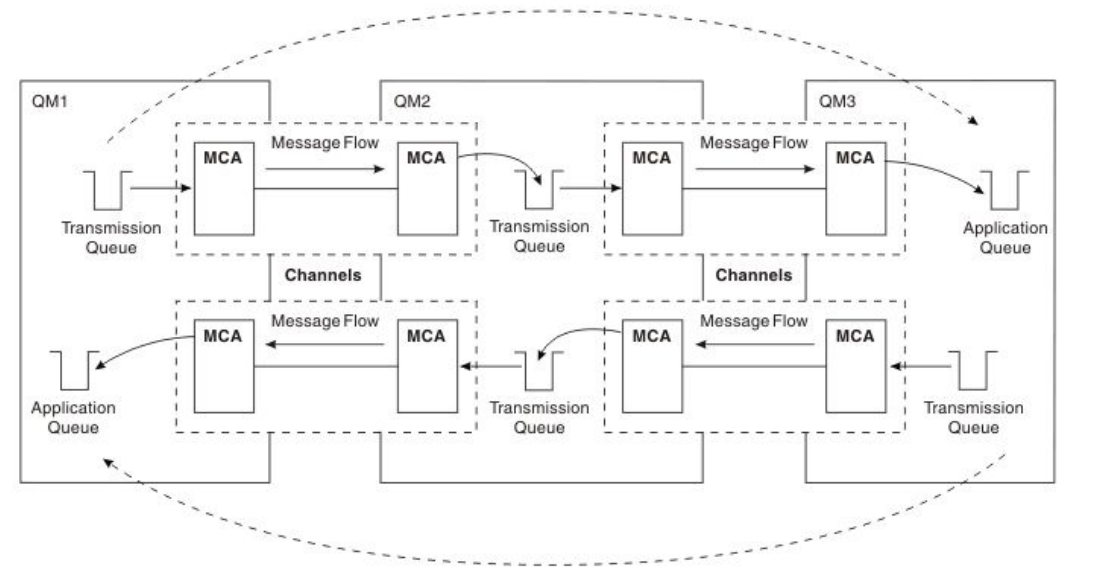
\includegraphics[scale=0.40]{img/overlay.png}
				\caption{Overlay network }
			\end{figure}
			Questa overlay network deve essere collegata e per farlo ogni entità deve essere a conoscenza degli indirizzi fisici associati ai nomi delle macchine partecipanti la rete e quindi delle loro rispettive code. Questo approccio \textbf{non risulta scalabile} e nel contesto di reti di grosse dimensioni porta ad evidenti \textbf{problemi gestionali}. Possiamo migliorare il modello di comunicazione delegando ai router la responsabilità di tenere traccia della topologia di rete e di aggiornare i binding (nome, indirizzo), mentre le altre entità partecipanti possiedono dei riferimenti statici al/ai router più vicino.
			
		\subsubsection{Eterogeneità: Message Brokers}
			I sistemi distribuiti possono essere eterogenei rispetto ai linguaggi utilizzati per realizzare le singole entità partecipanti. In questi casi è difficile definire un protocollo condiviso poichè è assente alla base un'accordo sul formato dei dati messaggi scambiati.\\
			Un \textbf{Message Broker} si comporta come un getway: si occupa di convertire i messaggi ricevuti in un formato consono a quello del ricevente. Nella pratica un message broker usa un repository di regole e programmi che permettono la conversione di un messaggio T1 in uno T2.
			Esempi di message brokers: 
			
	\subsection{Java RMI}
		Java RMI (\textbf{Remote Method Invocation}) è un framework che permette di implementare il modello RPC nel constesto di un sistema distribuito.
		\begin{figure}[h!]
			\centering
			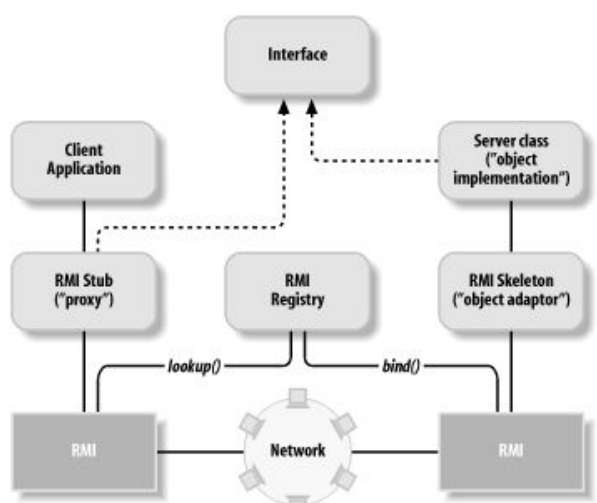
\includegraphics[scale=0.40]{img/rmi.png}
			\caption{Architettura di RMI}
		\end{figure}
		Il modello presenta 4 entità principali:
		\begin{itemize}
			\item \textbf{Interfaccia}: utilizzata per definire la risorsa remota;
			\item \textbf{Server}: implementa la risorsa remota (che sarà richiesta dal client);
			\item \textbf{Client}: richiede al server la risorsa remota.
			\item \textbf{Registro}: si occupa di gestire l'accesso alla risorsa remota.
		\end{itemize}
		Il \textbf{Registro}: è un servizio di \textbf{naming} che mappa i nomi simbolici degli oggetti remoti al loro stub. Il Server può registrare un oggetto remoto nel registro scrivendone il nome e l'indirizzo al quale è reperibile. Il client cerca l'oggetto remoto all'interno del registro.\\
		L'\textbf{interfaccia} specifica un contratto, ovvero le firme dei metodi che si possono invocare sull'oggetto remoto e che dunque ne regolano le modalità di utilizzo. \textbf{Per ogni oggetto} che vogliamo rendere accessibile attraverso la rete dobbiamo definire un'interfaccia che estenda l'interfaccia remota \textit{\textbf{java.rmi.remote}}. Le interfacce così definite dal server devono essere note anche al client in modo tale che egli possa operare sugli oggetti ricevuti dal server senza incorrere in errori di tipo. L'interfaccia remota serve solo ad indicare la possibilità di reperire gli oggetti che estendono tale interfaccia in remoto.\\
		Vediamo quali sono i passi per implementare un \textbf{RMI server}:
		\begin{enumerate}
			\item Implementare la classe remota definendo costruttore e metodi remoti (estendiamo la classe \textit{\textbf{java.rmi.server.UnicastRemoteObject }} e ne chiamiamo il costruttore per esportare l'oggetto);
			\item Creare un'istanza dell'oggetto remoto;
			\item Registrare tale oggetto remoto all'interno del registro. Per fare questo dobbiamo scegliere un identificativo unico (una stringa) per l'oggetto, che deve essere noto anche al client. Una volta ottenuto un riferimento al registry creiamo un binding tra quel nome e l'istanza dell'oggetto relativa. La classe \textit{\textbf{LocateRegistry}} permette di ottenere il riferimento al registro remoto o di crearne uno in ascolto sulla porta desiderata sullo stesso host del server (\textbf{\textit{createRegistry(int port), getRegistry(String host, int port )}}). 
		\end{enumerate}
		Per quanto riguarda il client i passi per l'implementazione sono i seguenti:
		\begin{enumerate}
			\item Localizzare il registro (stessi metodi della classe \textbf{LocateRegistry} indicati per il server);
			\item Utilizzare un nome simbolico per cercare l'oggetto remoto all'interno del registro;
			\item utilizzare l'oggetto remoto chiamandone i metodi. 
		\end{enumerate}
		Possiamo utilizzare RMI per implementare una comunicazione \textbf{sincrona} (il client aspetta fino al termine dell'invocazione remota). Possiamo ottenere una comunicazione \textbf{asincrona} utilizzando le \textbf{callback} il client invoca un oggetto remoto e passa la callback al server (un altro oggetto remoto).
		
	\subsection{gRPC}
		gRPC è un framework open source per l'implementazione del modello RPC:
		\begin{itemize}
			\item Si basa su i meccanismi di streaming messi a disposizione da \textbf{ HTTP/2};
			\item \textbf{Supporta molti linguaggi} grazie all'utilizzo di un \textbf{IDL} (Interface Definition Language).
			\item Si appoggia a \textbf{Protocol Buffer} che è un meccanismo per la serializzazione di strutture dati basato su un particolare formato binario che rendono i payload leggeri e veloci da trasmettere. Mette a disposizione un linguaggio proprio utilizzabile per definire interfacce indipendenti dal linguaggio.
		\end{itemize}
		I servizi messi a disposizione sono 4:
		\begin{itemize}
			\item \textbf{Unary RPCs}: Implementa uno scambio di messaggi \textbf{sincrono}.
			\item \textbf{Server streaming RPCs}: Un client invia richieste al server e riceve uno stream di messaggi (il client legge dallo stream fino a che non ci sono piu messaggi).
			\item \textbf{Client streaming RPCs}: Il client scrive una sequenza di messaggi e li manda al server utilizzando uno stream.
			\item \textbf{Bidirection streaming RPCs}: Entrambi i lati della comunicazione utilizzano uno stream in lettura/scrittura per inviare e ricevere messaggi.  
		\end{itemize}
		Il Workflow di gRPC è il seguente:
		\begin{itemize}
			\item \textbf{Definire un'interfaccia} utilizzando il Protocol Buffer Language ed il suo IDL (file di testo in formato \textbf{.proto});
			\item \textbf{Compilare} l'interfaccia per ottenere gli stub per client e server e le classi necessarrie alla serializzazione (si utilizza il comando \textbf{protoc}).
			\item \textbf{Integrare} gli stub con codice ad-hoc.
		\end{itemize}
		\begin{figure}[h!]
			\centering
			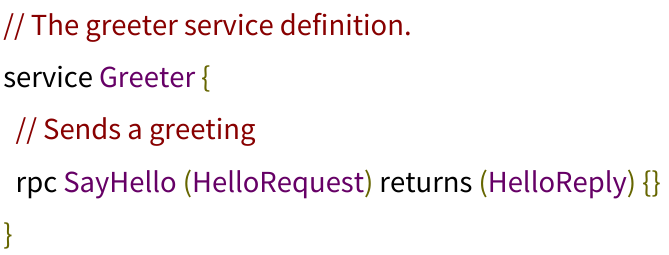
\includegraphics[scale=0.30]{img/idl.png}
			\caption{Definizione di un interfaccia con gRPC IDL}
		\end{figure}
		\begin{figure}[h!]
			\centering
			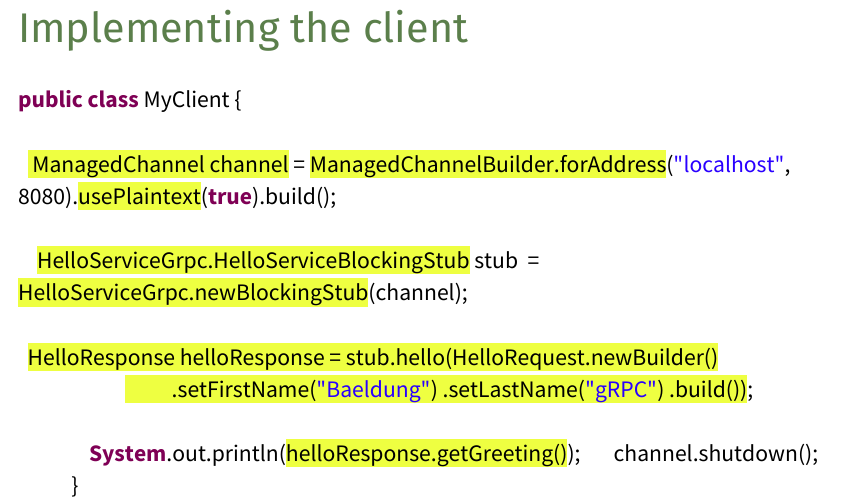
\includegraphics[scale=0.30]{img/grpc.png}
			\caption{Client in grpc}
		\end{figure}
		Un canale è una connessione virtuale per eseguire delle RPC, può avere zero o piu connessioni con l'endpoint. Il canale deve essere associato ad un numero di porta e da un indirizzo.
		
		
\section{Basic distributed algorithms}
	\subsection{Contesto}
		Il \textbf{contesto} nel quale operiamo è chiamato \textbf{ambiente distribuito}. Consiste in una collezione finita $\epsilon$ di \textbf{entità} che comunicano attraverso \textbf{messaggi} con lo scopo di raggiungere un \textbf{obiettivo comune}. Vediamo quali sono le componenti principali del modello:
		\begin{itemize}
			\item \textbf{Entità}: è l'unità computazionale di un ambiente distribuito, può essere vista come un processo, un agente, uno switch ecc. Ogni entità è equipaggiata con una memoria privata e non condivisa. La memoria è composta da un insieme di registri, tra i quali spiccano lo \textbf{status register}, che può assumere i valori di \textit{idle, Processing, Waiting}, e l'\textbf{input value register}. Inoltre è possibile settare un \textbf{alarm clock} locale che può essere resettato all'occorrenza.
			\item \textbf{Eventi esterni}: Il comportamento di un'entità è reattivo ed innescato da stimoli esterni. Questi possono essere:
			\begin{itemize}
				\item L'arrivo di un messaggio;
				\item Lo scadere dell'alarm clock;
				\item Impulsi spontanei.
			\end{itemize}
			L'ultimo è l'unico stimolo originato da forze che sono esterne al sistema (come esempio si riporta la richiesta ad un bancomat da parte dell'utente nel sistema ATM server- ATM client)
			\item \textbf{Azioni}: un'entità può svolgere le seguenti \textbf{operazioni}:
		\begin{itemize}
			\item Operazioni sulla memoria locale;
			\item Trasmissione dei messaggi;
			\item (re)set dell'alarm clock;
			\item Cambiare il valore del registro di stato.
		\end{itemize}
			Le azioni sono \textbf{atomiche} (non possono essere interrotte) e \textbf{finite} (devono terminare in tempo finito). L'azione speciale \textbf{nil} permette ad un'entità di non reagire ad uno specifico evento.
			\item \textbf{Comportamenti delle entità}: l'insieme $B(x)$ è una funzione $Statox Evento \rightarrow Azioni$ ovvero una funzione che ad una coppia stato-evento associa un comportamento (può definire un insieme di comportamenti \textbf{deterministico} o \textbf{non deterministico}). Un sistema è detto \textbf{simmetrico} se tutte le entità hanno lo stesso comportamento ($B(x) = B(y) \forall x,y \in E$). Tutti i sistemi possono essere resi simmetrici.
			\textbf{Comunicazioni:} guarda figure.
		\end{itemize}
		\begin{figure}[h!]
			\centering
			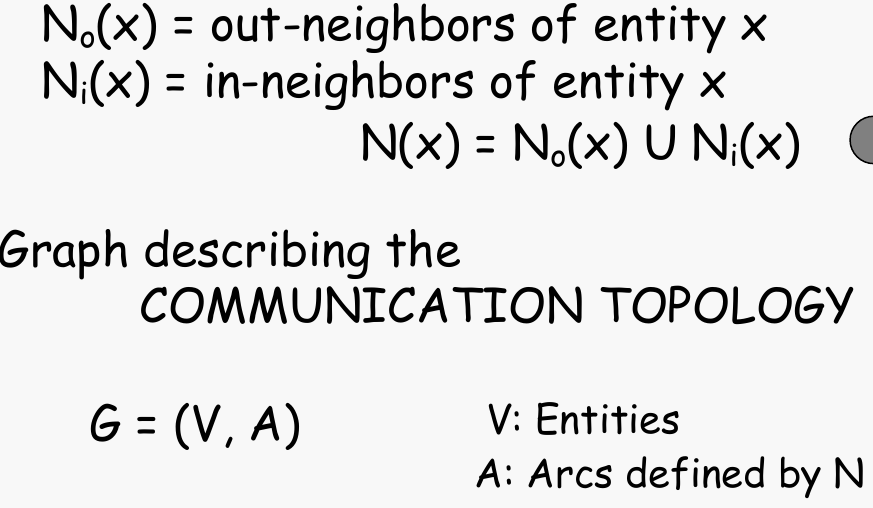
\includegraphics[scale=0.30]{img/comun.png}
			\caption{Come rappresentare la topologia di rete}
		\end{figure}
		\begin{figure}[h!]
			\centering
			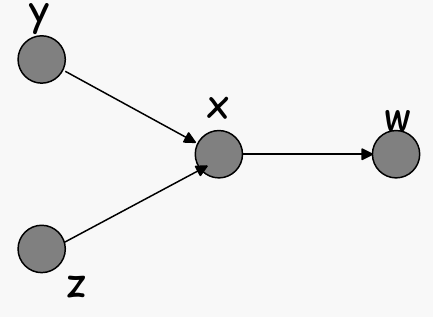
\includegraphics[scale=0.30]{img/graph.png}
			\caption{Topologia}
		\end{figure}
	
		\subsubsection{Assiomi}
			\begin{itemize}
				\item \textbf{Delay trasmissione messaggi}: in assenza di \textbf{fallimenti} un messaggio inviato da x ad un suon vicino y arriva in un tempo finito.
				\item \textbf{Orientamento Locale}: ogni entità può distinguere i suoi \textbf{out-neighbors} ( si utilizzano delle etichette sugli archi). Nella pratica un'entità sa da quale porta il messaggio gli è stato recapitato.
			\end{itemize}
			\begin{figure}[h!]
				\centering
				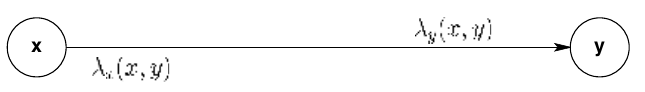
\includegraphics[scale=0.40]{img/lab.png}
				\caption{Labels}
			\end{figure}
		
		\subsubsection{Restrizioni}
			Si possono definire ulteriori proprietà o capacità in relazione ai compiti e agli obiettivi che il sistema distribuito si prepone di raggiungere. Tuttavia queste proprietà aggiuntive  limitano l'applicabilità reale del protocollo e dunque nella pratica rappresentano delle \textbf{restrizioni}. Vediamone alcune:
			\begin{itemize}
				\item \textbf{Ordine dei messaggi:} in assena di fallimenti, messaggi trasmessi nello stesso link arrivano nell'ordine d'invio.
				\item \textbf{Link bidirezionali}: $\forall x$ $N_{i}(x)=N_{o}(x)$ e $\forall y$ $\lambda_{x}(x,y) = \lambda_{x}(y,x	)$ 
				\item \textbf{Fault detection}:
				\begin{itemize}
					\item \textbf{Edge Failure Detection}: un'entità può individuare il fallimento di uno dei suoi link;
					\item \textbf{Entity Failure Detection}: un'entità può rilevare il fallimento di uno dei suoi vicini 	
				\end{itemize} 
				\item \textbf{Reliability restrinction}: 
				\begin{itemize}
					\item \textbf{Guaranteed delivery}: ogni messaggio inviato viene recapitato al mittente non corrotto;
					\item \textbf{Partial reliability}: garantisce l'assenza di fallimenti in futuro;
					\item \textbf{Total reliabilit}: non ci sono stati fallimenti e non ce ne saranno.
				\end{itemize} 
				\item \textbf{Strongly connected}: il grafo g che rappresenta la topologia è fortemente connesso.
				\item \textbf{Knowledge restrinction}
				\begin{itemize}
					\item conoscenza del numero di nodi;
					\item conoscenza del numero di link;
					\item conoscenza del diametro.
				\end{itemize}
			\end{itemize}
		
	\subsubsection{Tempo ed Eventi}
		Un evento esterno genera un'azione che dipende dallo stato dell'entità in questione. Un'azione può a sua volta generare un evento (per esempio l'operazione send genera un evento receiving). Un'ulteriore considerazione riguarda la possibilità che eventi generati in questo modo possano non occorrere nel caso in cui vi sia un fallimento del link di comunicazione. Ovviamente questi eventi se occorrono occorrono dopo del tempo (alla ricezione del messaggio per esempio). Eventi come \textbf{receiving} hanno un \textbf{delay non predicibile}. Un'esecuzione è descritta completamente dalla sequenza di eventi che è occorsa. Delay diversi porteranno ad esecuzioni differenti e dunque a risultati possibilmente diversi. Per convenzione tutti gli eventi spontanei sono generati al tempo $t=0$ prima che l'esecuzione abbia inizio.\\
		Definito $\alpha(x,t)$ lo stato del nodo x al tempo t, è importante evidenziare che:
		\begin{itemize}
			\item se un evento avviene in due esecuzioni diverse e gli stati $\alpha 1$ e $\alpha 2$ sono uguali, allora \textbf{il nuovo stato interno sarà lo stesso in entrambe le esecuzioni}.
			\item se un evento avviene al tempo t nei nodi x e y ed i loro stati $\alpha(x)$ e $\alpha(y)$ sono uguali, allora i nuovi stati di x e y saranno lo stesso stato.
		\end{itemize}
		
		
		\begin{figure}[h!]
			\centering
			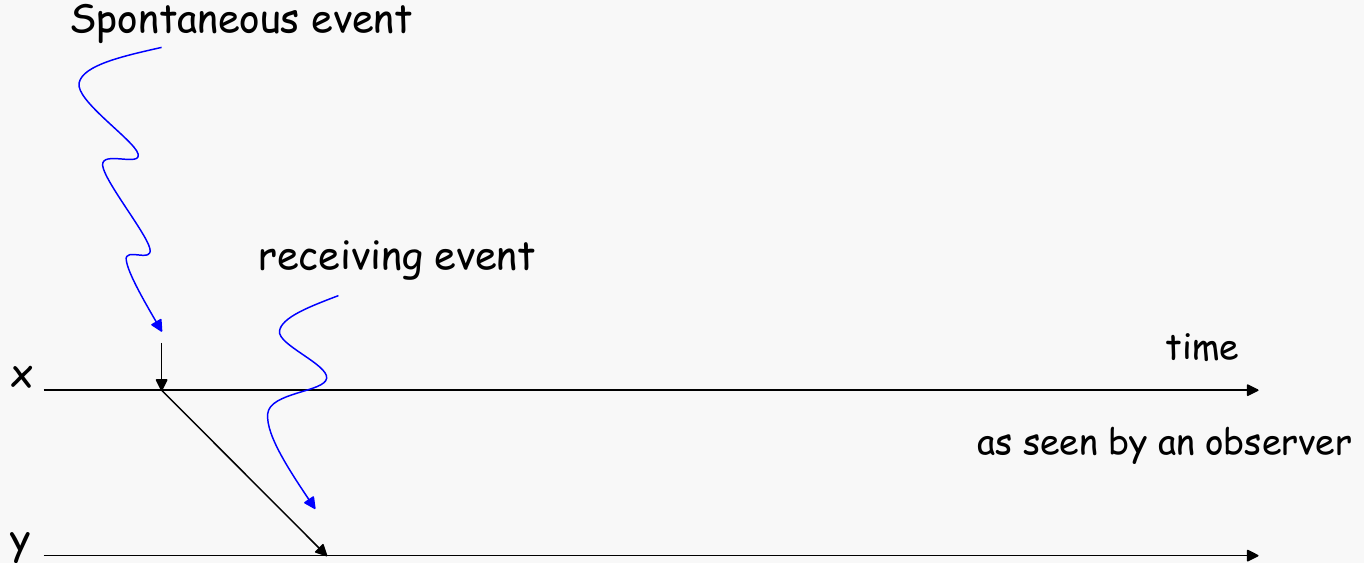
\includegraphics[scale=0.25]{img/event.png}
			\caption{Stato x Evento}
		\end{figure}
	
	\subsubsection{Livelli di Conoscenza}
		\begin{itemize}
			\item \textbf{Local knowledge}: $p \in LK_t[x]$ dove p è il contenuto della memoria locale di un'entità e tutte le informazioni derivabili da essa.
			\item \textbf{Implicit knowledge}: $p \in IK_t[W]\_ iff \exists x \in W$ $(p \in LK_t[x])$
			\item \textbf{Explicit knowledge}: $p \in EK_t[W]\_ iff \forall x \in W$ $(p \in LK_t[x])$
		\end{itemize}
		I \textbf{tipi di conoscenza} includono quelle \textbf{topologiche}, \textbf{metriche} (numero di nodi, diametro, eccentricità), \textbf{senso della direzione} (informazioni sui link, informazioni sulle label). Importante sottolineare come \textbf{al crescere delle conoscenze l'algoritmo diventi meno portatile}. Gli algoritmi generici non utilizzano nessuna conoscenza.     
	
	\subsection{Broadcast}
		Considerato un sistema distribuito nel quale solo il nodo x sia a conoscenza di una qualche informazione importante, il \textbf{problema del broadcast} consiste nel propagare questa informazione a tutti gli altri nodi. Una soluzione del problema deve essere valida a prescindere dal nodo \textbf{iniziatore}.
		
		\subsubsection{Flooding}
			\textbf{Assunzioni}: (\textbf{{BL, CN, TR}}) Bidirectional link, Connectivity (ogni entità è capace di raggiungere l'altra), Total reliability. + (\textbf{UI+}).\\
			Una soluzione al problema del broadcast è data dall'algoritmo \textbf{flooding}. L'idea è molto semplice: se un nodo è a conoscenza di qualcosa invia l'informazione ai suoi vicini. L'algoritmo è riportato in figura nella variante per la quale il mittente viene escluso dalla lista dei nodi ai quali inoltrare l'informazione ricevuta.
			\begin{figure}[h!]
				\centering
				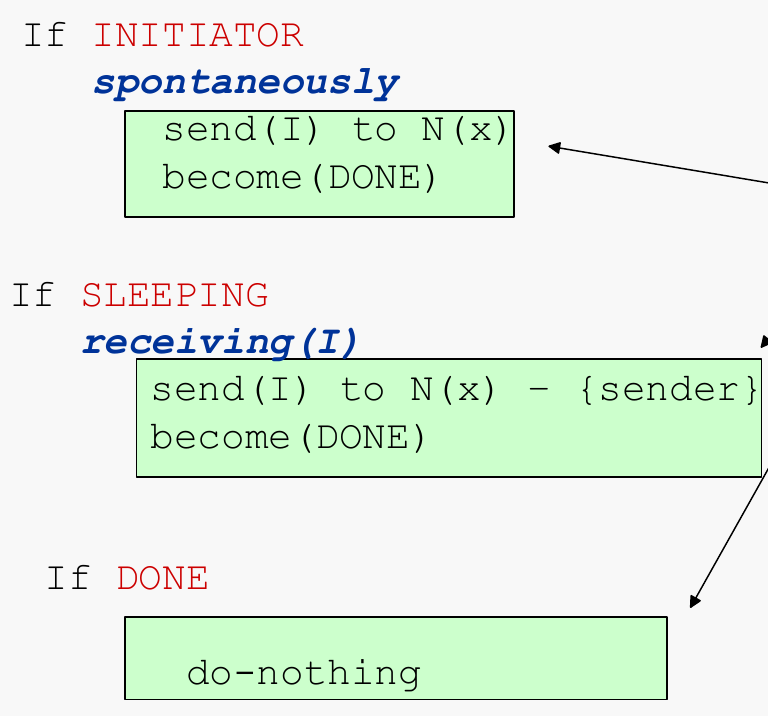
\includegraphics[scale=0.4]{img/flood.png}
				\caption{Algoritmo Flooding}
			\end{figure}
		L'algoritmo gode della proprità di \textbf{Termination}: l'algoritmo termina in tempo finito (local termination quando lo stato è \textit{done}). Garantita dal fatto che il grafo è connesso e che vale la proprietà di total reliability. Il caso peggiore si presenta quando il \textbf{grafo è completo}.\\
		Per quanto riguarda la \textbf{complessità dei messaggi}: vengono scambiati 2 messaggi per ogni link $$\sum_{x}^{}N(x)=2m \rightarrow 2m = O(m) $$ nello specifico:
		$$|N(s)|+\sum_{x\neq s}^{}(N(x)-1)=\sum_{x}^{}(N(x)-\sum_{x}^{}1) = 2m-(n-1)$$
		Per quanto riguarda la complessità in tempo abbiamo:
		$$r(s)=Max_x(d(x,s))=eccentricity \leq Diameter(G) \leq n-1$$
		con:
		$$Diameter(G)=Max_x(r(x))  $$
		
		
	\subsection{Flooding in reti con caratteristiche particolari}
		Un algoritmo che implementi il broadcast in un sistema distribuito varia la sua efficienza in base alla topologia di rete. Vediamo alcuni casi:
		\subsubsection{Broadcast in un Hypercube}
			Per $k=1$ un hypercube è un grafo che presenta due nodi collegati da un link.
			Un Hypercube $H_k$ di dimensione $k>1$ è ottenuto prendendo due hypercube di dimensione $k-1-H^{1}_k-1$ e collegando i nodi con nome uguale con un link etichettato. I nuovi nomi dei nodi sono ottenuti aggiungendo il prefisso 1 o il prefisso 0 ai nomi precedenti. Le label dei link sono ottenute contando i bit di differenza tra il nome dei due nodi collegati. Le etichette sono simmetriche rispetto ai nodi connessi dal link\\
			\begin{figure}[h!]
				\centering
				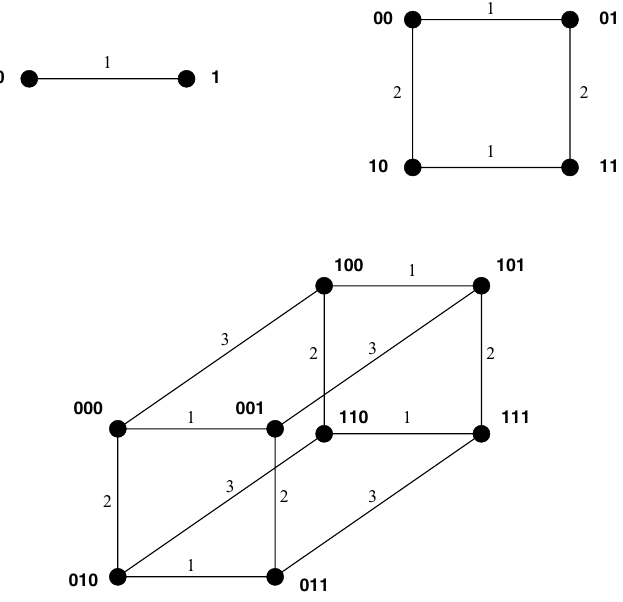
\includegraphics[scale=0.35]{img/hyper.png}
				\caption{Hypercube}
			\end{figure}
			\begin{figure}[h!]
				\centering
				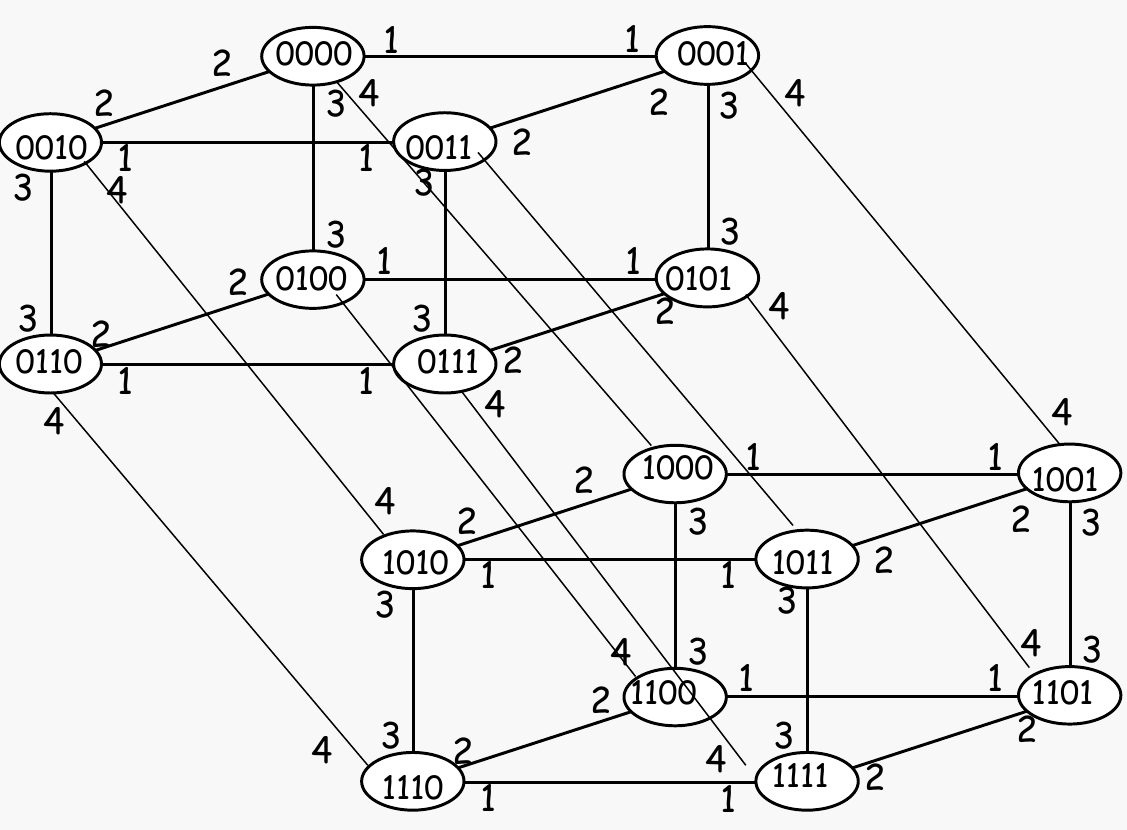
\includegraphics[scale=0.20]{img/hyper2.png}
				\caption{Costruzione hypercube}
			\end{figure}
			\textbf{\textit{Ricordiamo che i nomi dei nodi sono utilizzati solo a scopo descrittivo e non sono conosciuti dalle entità. Al contrario in nomi delle etichette sono noti alle entità per l'assioma di local orientation}.}\\
			Vediamo la \textbf{complessità} del flooding per questa particolare topologia. Un hypercube di dimensione $k$ ha $n=2^{k}$ \textbf{nodi}. Pertanto il \textbf{numero di link è}:
			$$m=nk/2= O(nlog(n)) $$ il costo del flooding è pertanto:
			$$2m-(n-1) = nlog(n)-(n-1)=(nlog(n)/2) +1=O(nlog(n))$$
			Possiamo utilizzare le proprietà topologiche dell'hypercube per ottenere un broadcast ancora più efficiente:
			\begin{enumerate}
				\item L'iniziatore invia il messaggio a tutti i suoi vicini;
				\item Un nodo che riceve un mesaggio dal link $l$, lo invia solo ai link con etichetta $l^{1}<l$ 
			\end{enumerate}
			Con questa modifica il flooding costerà soltanto (n-1) (messaggi).\\
			La \textbf{correttezza} dell'algoritmo è data dal seguente lemma: \textit{per ogni paio di nodi x,y esiste un path unico di etichette decrescenti}.
			\begin{figure}[h!]
				\centering
				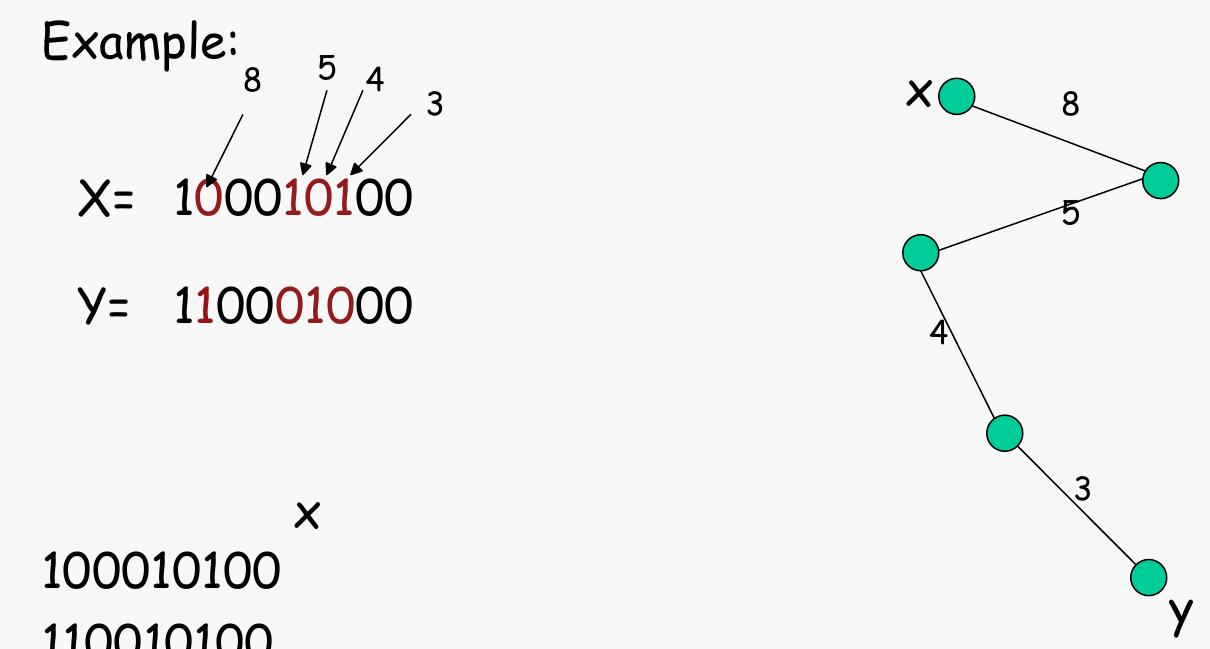
\includegraphics[scale=0.20]{img/hyper3.png}
				\caption{Lemma}
			\end{figure}
			Il risultato è che il messaggio crea uno \textbf{spanning tree} e ogni nodo è raggiunto da tale messaggio. La complessità risulta essere quella ottimale (n-1) perchè le entità ricevono l'informazione solo una volta. La complessità ideale in tempo è k poichè l'eccentricità di ogni nodo è k.
		\subsubsection{Broadcast in un grafo completo}
			Notiamo che nel caso di un grafo completo il flooding ha complessità 
			$$2m-(n-1)=O(n^{2}) $$ con complessità per i messaggi di:
			$$(n-1) $$
		\subsubsection{Lower bound}
			Torniamo al caso generale del broadcast e cerchiamo una limitazione inferiore per la sua complessità.\\ \textbf{Teorema}:\\
			\textit{Ogni algoritmo di broadcast richiede, nel caso pessimo, O(m) messaggi}.\\
			La prova avviene per contraddizione: sia A un algoritmo che esegue broadcast in meno di m(G) messaggi. In questo caso abbiamo almeno un link in G dove nessun messaggio inviato.
			
			VEDERE DIMOSTRAZIONE
			
	\subsection{Spanning tree construction}
		Per ottimizzare il costo di un algoritmo distribuito può essere una buona soluzione quella di ottenere una topologia di rete con particolari caratteristiche. è questo il caso degli \textbf{spanning tree}.\\
		Nella teoria dei grafi uno spanning tree T di un grafo \textbf{aciclico} è un suo sottografo che include tutti i vertici di G con il numero minore possibile di archi. Lo spanning tree per un grafo G \textbf{non è unico}.
		\subsubsection{Protocollo Shout}
			Grazie all'assioma di \textbf{local orientation} un'entità è consapevole solo delle etichette delle porte con le quali comunica con i suoi vicini. Inoltre sappiamo che i messaggi inviati ad un vicino sono prima o poi ricevuti dal destinatario (grazie all'assioma di \textbf{finite comunication delay} e la restrizione di \textbf{total reliability}). In questa configurazione iniziale un'entità ha bisogno di conoscere \textit{solo chi tra i suoi vicini è anche suo vicino nello spanning tree}. Vediamo la strategia utilizzata:
			\begin{enumerate}
				\item L'iniziatore \textbf{s} invia un messaggio ai suoi vicini \textbf{"\textit{sei tu il mio vicino?}"};
				\item un'entità $x\neq s$ risponde "\textit{\textbf{yes}"} solo la prima volta ed in questa occasione pone a tutti i suoi vicini la stessa domanda, altrimenti risponde "\textbf{\textit{no}}".
				\item Ogni entità termina quando ha ricevuto una risposta da tutti i vicini. 
			\end{enumerate}
			\begin{figure}[h!]
				\centering
				\includegraphics[scale=0.48]{img/shout.png}
				\caption{Algoritmo protocollo shout}
			\end{figure}
		Osservando la struttura dell'algoritmo è chiaro che risulta dalla composizione dei protocolli \textbf{flooding + reply}.
		\subsubsection{Correttezza}
			Sappiamo che flooding è corretto e dunque sappiamo che ogni entità riceverà Q e che per costruzione risponderà \textit{yes} o \textit{no} ad ogni Q che riceve.\\ 
			\textbf{ Per provare la correttezza dobbiamo provare che la sotto-rete $G^{1}$ definita da tutti gli alberi di vicini, è uno spanning tree di $G$.}\\
			Sappiamo che:
			\begin{itemize}
				\item Se $x$ è un tree-neighbor di $y$ allora $y$ è un tree-neighbor di $x$;
				\item Se $x$ invia \textit{yes}	ad $y$, allora $x$ è un tree-neighbor di $y$ ed è connesso all'iniziatore da una catena di \textbf{yes};
				\item Ogni $x$ (a parte l'iniziatore) risponde \textit{yes} solo una volta (quando diventa \textbf{active} risponde no ad ogni richiesta).
			\end{itemize}
			\textbf{Poichè ogni entità $x \neq y$ invia un solo \textit{yes} allora $G^{1}$ contiene tutte le entità di G, è connesso e non contiene cicli e dunque è uno spanning tree di G.}\\
			Importante ricordare che Shout termina per \textbf{terminazione locale} ovvero che ogni entità conosce quando la propria esecuzione è terminata (quando entra nello stato \textbf{done}). Nemmeno l'iniziatore è a conoscenza della \textbf{terminazione globale} (situazione molto comune in un algoritmo distribuito).
		\subsubsection{Costo computazionale}
			Dal momento che shout è definito come flood + reply studiarne la complessità risulta essere molto semplice: 
			$$Message(SHOUT) = 2Message(FLOOD) = 4m-2n+2 $$
			Dal momento che $O(m)$ è un \textbf{lower bound} diciamo che shout è \textbf{asintoticamente ottimo.}
			Nello specifico:
			\begin{figure}[h!]
				\centering
				\includegraphics[scale=0.25]{img/shout1.png}
				\caption{Shout: possibili situazioni}
			\end{figure}
			\begin{figure}[h!]
				\centering
				\includegraphics[scale=0.25]{img/shoutmess.png}
				\caption{Totale dei messaggi Q (sei mio vicino?)}
			\end{figure}
			\begin{figure}[h!]
				\centering
				\includegraphics[scale=0.25]{img/shoutmess1.png}
				\caption{Totale dei messaggi Q: formula}
			\end{figure}
			\begin{figure}[h!]
				\centering
				\includegraphics[scale=0.250]{img/numbno.png}
				\caption{Totale dei messaggi no}
			\end{figure}
			\begin{figure}[h!]
				\centering
				\includegraphics[scale=0.25]{img/numbyess.png}
				\caption{Totale dei messaggi yess}
			\end{figure}
			\begin{figure}[h!]
				\centering
				\includegraphics[scale=0.25]{img/totmess.png}
				\caption{Totale dei messaggi scambiati}
			\end{figure}
		
			\newpage
		\subsubsection{Possibili migliorie}
			\textit{Possiamo modificare l'algoritmo in modo tale da eliminare i messaggi \textbf{no}}. Ricordiamo che i delay di consegna dei messaggi sono assunti finiti ma sono per definizione impredicibili. Non possiamo dunque fare a meno dei messaggi di no in quanto non possiamo semplicemente attendere lo scadere  dell'upper-bound di consegna dei messaggi per capire se un'entità risponderà $yes$ o meno. la in quanto sono utilizzati per la terminazione local Per farlo si interpretano i messaggi Q ricevuti come dei no (vedi figura).  La complessità si riduce a:
			$$Messages(SHOUT) = 2si o menom$$
			\begin{figure}[h!]
				\centering
				\includegraphics[scale=0.25]{img/shoutmod.png}
				\caption{Shout senza messaggi no}
			\end{figure}
			Un'altra possibile miglioria è implementata con lo scopo di ottenere \textbf{terminazione globale} per l'algoritmo. Si introducono degli \textbf{ACK} che permettono di notificare alla root quando terminare globalmente l'algoritmo. L'idea è quella di introdurre una procedura \textbf{CHECK} che permette ad un nodo, alla ricezione di un messaggio e qualora tutti i propri vicini abbiano risposto, di controllare di essere una \textbf{foglia}: in caso affermativo la foglia invia un \textbf{ACK} al proprio parent. Il parent attende di ricevere un ACK dai tutti i figli per inviare un ACK al padre. Una volta che l'ACK giunge alla root, quest'ultima fa partire dei messaggi di \textbf{termination}. In poche parole gli ACK si muovono dalle foglie verso la radice, mentre i messaggi di termination svolgono il percorso contrario.
			\begin{figure}[h!]
				\centering
				\includegraphics[scale=0.30]{img/shoutterm.png}
				\caption{Algoritmo Shout con global termination 1}
			\end{figure}
			\begin{figure}[h!]
				\centering
				\includegraphics[scale=0.30]{img/shoutterm2.png}
				\caption{Algoritmo Shout con global termination 2}
			\end{figure}
			\begin{figure}[h!]
				\centering
				\includegraphics[scale=0.30]{img/shoutterm3.png}
				\caption{Algoritmo Shout con global termination}
			\end{figure}
		\newpage
		
		\subsubsection{Iniziatore mutliplo}
			Abbiamo implementato l'algoritmo \textit{shout} assumendo l'esistenza di un \textbf{iniziatore unico}. Tuttavia questa è un'assunzione molto forte da considerare per un sistema distribuito. In figura si mostra cosa accade nel caso di multipli iniziatori: presi i nodi $x$, $y$, $z$ connessi l'uno con l'altro, con $x$ e $y$ iniziatori, si vede facilmente che se il messaggio Q inviato da $x$ arriva prima a $z$ allora i link $(x,y)$ e $(y,z)$ non saranno presenti nello spanning tree. L'algoritmo di fatto costruisce una \textbf{spanning forest} non connessa.
			\begin{figure}[h!]
				\centering
				\includegraphics[scale=0.35]{img/multip.png}
				\caption{Iniziatori multipli in Shout}
			\end{figure}
			Questo risultato particolare è avvallato dal \textbf{risultato di impossibilità}:\\
			\textbf{Teorema:} \textit{il problema della costruzione di un spanning tree è deterministicamente impossibile assumendo R.} \\
			Ciò significa che non esiste un protocollo deterministico che termina sempre in tempo finito.
			La prova viene data per assurdo: l'idea è che le entità hanno lo stesso codice e perciò, iniziando simultaneamente nello stesso stato, riceveranno gli stessi messaggi e svolgeranno le stesse computazioni, trovandosi sempre negli stessi stati (tutte le entità sono iniziatori). Il protocollo per essere corretto deve terminare in questa configurazione: x ha la label 2 nella lista, y ha la label 1, mentre z le ha tutte e due. L'assurdo si rileva nel fatto che le entità avrebbero valori distinti anche se gli stati e le computazioni svolte risultano le stesse. \\
			\begin{figure}[h!]
				\centering
				\includegraphics[scale=0.35]{img/imposprove.png}
				\caption{Prova risultato impossibilità}
			\end{figure}
			Se vogliamo costruire uno spanning tree in un contesto distribuito abbiamo dunque bisogno di un algoritmo che esegue la \textbf{leader election}.
			
		\subsubsection{SPT: Depth First Search}
			Sappiamo che una visita in profondità di un grafo restituisce uno spanning tree di tale grafo.
			L'idea è quella di utilizzare un token per identificare il nodo corrente: 
			\begin{itemize}
				\item Quando un nodo viene visitato per la prima volta, tiene traccia di chi è il mittente ed inoltra il token ad uno dei suoi vicini non ancora visitati.
				\item Quando un vicino riceve il token, se è già stato visitato marca l'arco come \textbf{back-edge} e restituisce il token, altrimenti inoltra sequenzialmente il token a tutti i suoi vicini sequenzialmente.
				\item Se non ci sono più vicini non visitati ritorna il token (\textbf{reply}) al nodo dal quale per primo ha ricevuto il token.
				\item Una volta ricevuto un reply, inoltra il token ad un altro vicino non visitato. 
			\end{itemize}
			\begin{figure}[h!]
				\centering
				\includegraphics[scale=0.3]{img/dfs.png}
				\caption{Algoritmo DFS 1}
			\end{figure}
			\begin{figure}[h!]
				\centering
				\includegraphics[scale=0.3]{img/dfs2.png}
				\caption{Algoritmo DFS 2}
			\end{figure}
		
			FARE IMMAGINE CON SLIDE DA 30 a 41\\
			
			Per quanto riguarda la \textbf{complessità in messaggi} abbiamo che i messaggi per link sono 2 ( il destinatario del token risponde return se visitato la prima volta o back se già visitato). Dunque:
			$$2m = O(m) $$ con $$O(m) = lower bound $$
			Allo stesso modo la \textbf{complessità in tempo} risulta essere: 
			$$2m = O(m) $$ 	con $$O(n) = lower bound $$
		
		\subsubsection{DF: migliorie}
			Una prima idea è quella di eliminare i messaggi \textbf{back} che costituiscono la maggioranza del totale dei messaggi inviati. Per farlo utilizziamo \textbf{notification} e i messaggi di \textbf{ACK}. 
			\begin{itemize}
				\item L'idea è che il nodo corrente informa i suoi vicini di essere stato visitato.
				\item I vicini rispondono con messaggi di ACK. 
				\item Il mittente dunque segna tutti gli archi dal quale riceve risposta come back-edge.
				\item Sceglie un vicino da visitare e marca quel link come appartenente allo spanning tree. 
			\end{itemize}
			
			INSERIRE IMMAGINI SLIDE 44-48\\
			
			Per quanto riguarda la \textbf{complessità in messaggi} abbiamo che ogni entità riceve un \textbf{token} ed invia un \textbf{return} $$2(n-1)$$
			Inoltre ogni entità invia 1 \textbf{visited} a tutti i vicini tranne al mittente (lo stesso vale per i messaggi di ACK).
			$$\sum|N(s)|+\sum_{x\neq s}(|N(x)|-1) $$
			Il totale è dunque $4m $
			Per quanto riguarda la \textbf{complessità in tempo} abbiamo che i l'invio dei Token e il Return sono inviati sequenzialmente con complessità $2(n-1)$ mentre l'invio degli ack e dei messaggi visited è svolto in parallelo con complessità $2n$. Il totale risulta $$4n-2	$$
			
			FINIRE DF++\\
			
\subsection{Computazione negli alberi}		
	In questa sezione è analizzato il contesto delle computazioni distribuite in una topologia in forma di \textbf{albero}. Anche in questo caso valgono le restrizioni standard definite da \textbf{R}, in aggiunta ogni nodo sa se è una \textbf{foglia} o un \textbf{nodo interno} (se ha un solo vicino o più di uno).
	
	\subsubsection{Saturation}  
		La \textbf{Saturazione} è una tecnica base che può essere utilizzata come strumento di partenza per eseguire computazioni in un sistema distribuito. Il protocollo si declina in 3 parti: \textbf{Attivazione}, \textbf{Saturazione}, \textbf{Risoluzione}.
		La fase di risoluzione dipenderà dall'applicazione specifica del protocollo (definisce cosa facciamo con i messaggi di saturation ricevuti) anche se solitamente viene utilizzata come fase di notifica per tutte le entità (con lo scopo di ottenere \textit{local termination}). Un protocollo "troncato" come questo è chiamato \textbf{plug-in} (un protocollo nel quale non tutte le entità entrano in stato terminale). Per far si che diventi un protocollo è necessario definire ulteriori azioni da svolgere. \textit{\textbf{Il protocollo può essere avviato da un qualsiasi numero di initiator.}} Vediamo le fasi in dettaglio:
		\begin{enumerate}
			\item \textbf{Attivazione}: questa fase è un semplice \textbf{\textit{wake-up}}. Ogni initiator invia un messaggio di wake-up a tutti i suoi vicini e diventa \textit{active}. Ogni non initiator che riceve il messaggio diviene active a sua volta e inoltra il messaggio ai suoi vicini (escluso il mittente del messaggio)). I nodi già attivi ignorano altri messaggi di wake up. In \textbf{tempo finito} tutti i nodi divengono attivi, incluse le foglie (per le assunzione di \textbf{total reliability} e l'assioma di \textbf{finite comunication delay})
			\item \textbf{Saturazione}: questa fase è inizializzata dalle foglie che inviano il messaggio \textbf{M} di saturazione al loro unico vicino (il parent), entrando così nello stato di \textbf{\textit{processing}}. Invece, ogni nodo intermedio attende di ricevere un messaggio di saturation da tutti i suoi vicini meno uno. All'ultimo vicino rimasto ed identificato dunque come il parent, il nodo intermedio invia un messaggio di saturation (entrando nello stato \textit{processing}). Se un nodo nello stato di processing riceve un messaggio dal parente allora entra nello stato \textit{\textbf{saturated}}.
			\item \textbf{Risoluzione}: dipende dall'applicazione.	
		\end{enumerate}	
		
		\begin{figure}[h!]
			\centering
			\includegraphics[scale=0.33]{img/sat1.png}
			\caption{Algoritmo Saturazione 1}
		\end{figure}
		\begin{figure}[h!]
			\centering
			\includegraphics[scale=0.3]{img/sat2.png}
			\caption{Algoritmo Saturazione 2}
		\end{figure}
		\begin{figure}[h!]
			\centering
			\includegraphics[scale=0.3]{img/sat3.png}
			\caption{Algoritmo Saturazione 3}
		\end{figure}
		
		\subsubsection{Prova di correttezza}
			\textbf{Lemma}: \textit{Esattamente due nodi in stato di processing diventeranno saturati, inoltre questi nodi sono vicini ma anche l'uno il parent dell'altro}\\
			
			\textbf{Prova:} dzal codice sappiamo che un nodo invia il messaggio M solo al suo parente e diviene saturato solo se riceve un messaggio M dal parent. Scegliendo arbitrariamente un nodo della rete $x_{i}$, se attraversiamo gli up-edges (archi che collegano $x_{i}$ al proprio parent) prima o poi troviamo un nodo saturato $s_1$ (questo perchè non ci sono loop nel grafo). Il nodo $s_1$ è diventato saturato perchè ha ricevuto un messaggio da un nodo $s_2$ mentre era nello stato di processing (dunque ha già ricevuto M da un altro nodo quando era active). Dal punto di vista di $s_2$ questo significa che egli è nello stato processing e che considera $s_1$ il suo parent. Dunque, quando $s_2$ riceve un messaggio da $s_1$ questo diventa saturato a sua volta (i due nodi sono l'uno il parent dell'altro). Considerando il caso in cui i nodi saturati sono più di due allora significherebbe che esistono due nodi x,y  saturati per i quali $d(x,y)\leq 2$. Tuttavia se consideriamo un nodo z tra i due nodi x,y vediamo che z non può inviare il messaggio M ad entrambi i nodi e dunque uno dei nodi non può essere saturato. \\
			
			\textbf{Importante}: è impredicibile quale coppia di nodi divenga saturata, questo per via dei delay di consegna dei messaggi ( ovviamente incide anche la scelta degli iniziatori).
			\begin{figure}[h!]
				\centering
				\includegraphics[scale=0.3]{img/satprov.png}
				\caption{Algoritmo Saturazione: prova}
			\end{figure}
		
		\subsubsection{Complessità}
			\begin{figure}[h!]
				\centering
				\includegraphics[scale=0.3]{img/satmess.png}
				\caption{Algoritmo Saturazione: complessità caso peggiore}
			\end{figure}
			\begin{figure}[h!]
				\centering
				\includegraphics[scale=0.3]{img/satmess2.png}
				\caption{Algoritmo Saturazione: complessità caso generale con n iniziatori}
			\end{figure}
		
		\subsubsection{Ricerca del minimo con saturazione}
			In questa sezione vediamo come si può implementare la fase di risoluzione del protocollo per la ricerca del minimo. In questa configurazione ogni nodo possiede un valore $v(x)$, al termine dell'algoritmo ogni nodo è consapevole di possedere il valore minimo ed entra nello stato appropriato (\textit{minimum} o \textit{large}). Più entità possono avere il valore minimo.\\
			Il problema può essere risolto, nel caso di un rooted tree (esiste un nodo speciale che è la radice e abbiamo orientamento degli archi) eseguendo \textbf{convergecast}: a partire dalle foglie i nodi determinano il valore minimo e lo inviano verso la radice. Il minimo è dunque individuato dalla radice che si occupa di comunicarlo in broadcast agli altri nodi. \textbf{\textit{Assumere l'esitenza di una radice è un'assunzione molto forte:  equivale ad assumere l'esistenza di un leader all'interno della topologia.}} \\
			Per questo motivo usiamo \textbf{saturation} per risolvere il problema senza bisogno di queste informazioni. L'unica modifica effettuata riguarda la fase di processing:
			\begin{figure}[h!]
				\centering
				\includegraphics[scale=0.3]{img/mincomp.png}
				\caption{Ricerca minimo con Saturazione: complessità}
			\end{figure}
		
		\subsubsection{Computazione distribuita di funzioni}
			Il problema vede la computazione di una funzione all'interno di un sistema nel quale i suoi argomenti sono distribuiti nei nodi della topologia. \\
			Assumiamo la funzione \textit{f} essere \textit{associativa } e \textit{commutativa}. Questo tipo di funzioni, assieme ai suoi parametri, sono dette \textbf{Semigruppi commutativi}. 
			\begin{figure}[h!]
				\centering
				\includegraphics[scale=0.3]{img/semigrup.png}
				\caption{Semigruppi commutativi}
			\end{figure}
			\begin{figure}[h!]
				\centering
				\includegraphics[scale=0.3]{img/distfun.png}
				\caption{Algoritmo computazione distribuita di funzioni 1}
			\end{figure}	
			\begin{figure}[h!]
				\centering
				\includegraphics[scale=0.3]{img/distfun1.png}
				\caption{Algoritmo computazione distribuita di funzioni 2}
			\end{figure}
			\begin{figure}[h!]
				\centering
				\includegraphics[scale=0.3]{img/distfun1.png}
				\caption{Computazione distribuita di funzioni: complessità}
			\end{figure}
		
	\subsection{Leader Election}
		In molte applicazioni distribuite si richiede che una singola entità  si comporti temporaneamente come un controller centrale che coordina l'esecuzione dei task. I\textit{l problema è dunque quello di modificare la configurazione iniziale del sistema, nel quale tutte le entità sono nello stesso stato, in una configurazione finale nella quale tutte le entità sono nello stesso stato meno che una: il} \textbf{Leader}. 
		\subsubsection{Risultato di impossibilità}
			Ricordiamo le restrizioni: \textbf{Bidirectional Link}, \textbf{Connettività}, \textbf{Total Reliability}.\\
			\textit{Non esiste un protocollo deterministico per il problema della leader election che termini sempre in tempo finito.}
			\begin{itemize}
				\item Due entità x e y sono inizialmente nello stesso stato (available).
				\item Se un protocollo che risolve tale problema deve farlo in tutte le possibili configurazioni di \textbf{delay di consegna} dei messaggi. Consideriamo una comunicazione \textbf{sincrona} (delay di consegna unitari): se entrambe le entità iniziano l'esecuzione del protocollo nello stesso momento allora essi scambieranno gli stessi messaggi ed eseguiranno dunque le stesse regole, terminando entrambe nello stesso stato.
				\item \textbf{Se uno dei due diventa leader anche l'altro lo diventa contraddicendo il requisito per il quale al termine del protocollo dobbiamo avere un solo iniziatore.}
				\item P non è una soluzione valida.
			\end{itemize}
		Dobbiamo introdurre dunque altre restrizioni che permettano di rompere la simmetria che si verifica nel comportamento delle entità. Si potrebbe pensare di introdurre la restrizione di \textbf{UI+} ma in questo modo sposteremmo il problema (sarebbe come dire che riusciamo sempre ad eleggere un leader se c'è n'è già uno). L'idea è dunque quella di poter distinguere in modo univoco le entità dotandole di un \textbf{identificativo unico} (o nome globale). \\
		In questo modo si ha quello che chiamiamo \textbf{standard set for election}.
	
		\subsubsection{Election negli alberi}
			Vediamo alcune delle possibili strategie:
			\begin{itemize}
				\item Trovare il minimo (con l'introduzione degli ID la ricerca del minimo è di fatto un algoritmo di leader election.
				\item Trovare il minimo tra gli iniziatori
				\item Costruire uno spanning tree con radice.
			\end{itemize}
			
			Si può vedere che eleggere il minimo iniziatore all'interno dell'albero ha la stessa complessità di trovare il valore minimo utilizzando la tecnica della saturazione. La complessità in messaggi è la seguente: 
			$$3n+k^*-4 \leq 4n-4 $$ 
			Per quanto riguarda la strategia che vede la \textbf{costruzione di un albero con radice } possiamo anche in questo caso applicare la tecnica della saturazione (ricordiamo che abbiamo già una topologia ad albero dobbiamo solo eleggere la radice). Ricordiamo che utilizzando la \textit{full saturation} si ottengono inizialmente due soli nodi saturati. Il risultato è che avremo un albero con due radice: dobbiamo scegliere una delle due. \textbf{In poche parole diciamo che il problema di eleggere un leader tra tutti i nodi viene ridotto al problema di eleggere il leader tra due nodi (non ci importa che questi abbiano effettivamente il valore  minimo).}\\
			\begin{figure}[h!]
				\centering
				\includegraphics[scale=0.40]{img/elec.png}
				\caption{Root Election}
			\end{figure}
			La complessità in messaggi risulta analoga a quella relativa al protocollo \textbf{full saturation con notification}.
			$$M[Tree:ElectRoot] = 3n+k^*-2 \leq 4n-2$$ 
			Volendo fare un'analisi più (con granularità più) fine dobbiamo considerare i \textbf{bit spesi }per ogni messaggio. Da questo punto di vista l'algoritmo per l'elezione della radice è molto migliore rispetto a quello di elezione del minimo: solo gli n messaggi della fase di saturazione trasmettono un valore, gli altri sono semplici segnali.  
			\begin{figure}[h!]
				\centering
				\includegraphics[scale=0.3]{img/bitcom.png}
				\caption{Bit complexity}
			\end{figure}  
		\subsubsection{Leader election in un anello: All the Way}
			Consideriamo ora un'altra topologia classica nel contesto dei sistemi distribuiti: l'\textbf{anello}. Le proprietà caratteristiche di un anello sono le seguenti:
			\begin{itemize}
				\item Numero delle entità = numero link;
				\item Topologia simmetrica (tutti i nodi sono identici)
				\item Ogni entità ha due vicini
			\end{itemize}
			Il primo algoritmo trattato è \textbf{all the way}. L'idea è la seguente:
			\begin{itemize}
				\item Quando un'entità inizia la sua esecuzione sceglie uno dei due vicini ed invia un messaggio Election contenente il suo ID.
				\item Quando un'entità riceve un messaggio da uno dei due vicini, lo inoltra all'altro vicino. Inoltre invia un altro messaggio (se non l'ha già fatto) con il proprio ID.
				\item Ogni entità tiene traccia del più piccolo valore ricevuto.
			\end{itemize}
			In poche parole ogni entità invia un messaggio che attraversa tutta la topologia. ne consegue, ovviamente, che prima o poi tutte le entità vedano l'ID di tutte le altre entità (finite comunication delay, total reliability).
			\begin{figure}[h!]
				\centering
				\includegraphics[scale=0.25]{img/ring2.png}
				\caption{All the way}
			\end{figure}
			\begin{figure}[h!]
				\centering
				\includegraphics[scale=0.30]{img/allalg.png}
				\caption{All the way 1}
			\end{figure}
			\begin{figure}[h!]
				\centering
				\includegraphics[scale=0.30]{img/allalg1.png}
				\caption{All the way 2}
			\end{figure}
			
		\subsubsection{All the way: correttezza e terminazione}
			Idealmente potremmo dire che ogni entità termina quando riceve indietro il proprio id. Questo ragionamento è suggerito dal fatto che, considerando un nodo x, ogni messaggio inviato da un suo vicino qualsiasi deve attraversare un numero minore di nodi per raggiungerlo. Questo ragionamento risulta incorretto a meno di introdurre un'ulteriore assunzione: \textbf{message ordering}. Per quest'ultima assumiamo che tutti i canali di comunicazione implementino una politica \textbf{FIFO} e che dunque i messaggi vengano inoltrati da ogni entità nello stesso ordine in cui sono ricevuti. In questa configurazione un'entità \textit{conta quanti valori diversi riceve e quando il counter è uguale a n termina la propria esecuzione}. Un ulteriore problema è che l\textbf{e entità non conoscono il numero n di nodi facenti parte dell'anello}. La soluzione è quella di utilizzare un secondo counter, stavolta contenuto in ogni messaggio, incrementato da ogni altra entità che lo riceve: in questo modo quando x riceve indietro il proprio messaggio conosce anche il numero di nodi della rete. Quanto detto sull'algoritmo è valido anche nel caso di considerare link bidirezionali.
			La \textbf{complessità} dell'algoritmo è riassunta brevemente in figura.  
			\begin{figure}[h!]
				\centering
				\includegraphics[scale=0.30]{img/allcomp.png}
				\caption{All the way: complessità}
			\end{figure}
		
		\subsubsection{AsFar (as it can)}
			Le assunzioni per questo protocollo sono: \textbf{Unidirectional/Bidirectional link, Different ids, Local Orientation}.\\
			L'idea è molto semplice: \textbf{non è necessario ricevere e inoltrare messaggi che hanno un ID più grande degli id che sono stati visti.}
			\begin{figure}[h!]
				\centering
				\includegraphics[scale=0.30]{img/asfar.png}
				\caption{AsFar}
			\end{figure}
			\begin{figure}[h!]
				\centering
				\includegraphics[scale=0.30]{img/asfar3.png}
				\caption{AsFar: algoritmo 1}
			\end{figure}
			\begin{figure}[h!]
				\centering
				\includegraphics[scale=0.30]{img/asfar4.png}
				\caption{AsFar. algoritmo 2}
			\end{figure}
			
		\subsubsection{AsFar: terminazione}
			Sappiamo che il messaggio con l'ID più piccolo sarà sempre inoltrato dagli altri nodi, ritornando al mittente originario. Inoltre sappiamo che ogni altro messaggio (con ID più grande) sarà prima o poi terminato da un'altro nodo della rete. Questi due caratteristiche del protocollo ci forniscono un meccanismo di terminazione. Tuttavia solo l'entità che vede tornare indietro un messaggio con il proprio ID sa di essere il leader e dunque dovrà comunicarlo alle altre entità della topologia.
		\subsubsection{AsFar: complessità}
			Rispetto ad all the way il protocollo impiega un numero minore di messaggi. Il percorso di un messaggio all'interno della topologia viene interrotto nel caso in cui si trovi un id più piccolo, dunque il numero totale di messaggi dipende da come gli ID sono dislocati nell'anello.\\
			\textbf{Caso peggiore}\\
			Il caso peggiore risulta quello nel quale gli ID sono dislocati in ordine crescente e i messaggi sono inviati nella direzione "crescente". In questo caso non è importante il valore reale di un id ma solo se è più piccolo o più grande rispetto agli altri. Quello che è importante è dunque il \textbf{rank} (\textbf{i}) degli ID. 
			\begin{itemize}
				\item Nel caso $i=1$ (rango più piccolo) abbiamo che il messaggio si propaga nella rete fino a tornare al mittente impiegando $n$ messaggi.
				\item Nel caso $i=2$ il messaggio viene fermato solo dall'entità che ha rango $i=1$ impiegando $(n-1)$ messaggi.
				\item In generale nel caso $i+1$ si impiegano $(n-i)$ messaggi 
			\end{itemize}
			\begin{figure}[h!]
				\centering
				\includegraphics[scale=0.25]{img/worscas.png}
				\caption{AsFar: complessità caso pessimo}
			\end{figure}
			\begin{figure}[h!]
				\centering
				\includegraphics[scale=0.30]{img/ascom.png}
				\caption{AsFar: complessità caso pessimo}
			\end{figure}
			Abbiamo diminuito il numero di messaggi di almeno metà. Dal punto di vista teorico non è un grande risultato ma dal punto di vista pratico può essere considerato soddisfacente. Inoltre abbiamo per ora analizzato solo il caso pessimo.\\
			\textbf{Caso migliore}
			La dislocazione degli id è quella del caso pessimo ma i messaggi sono inviati nella direzione decrescente. Complessità in figura. Il caso medio ha complessità $O(nlog(n))$
			\begin{figure}[h!]
				\centering
				\includegraphics[scale=0.30]{img/asbest.png}
				\caption{AsFar: complessità caso migliore}
			\end{figure}
		
		\subsubsection{Controlled Distances}
			Le assunzioni per il protocollo sono: \textbf{Bidirectional ring}, \textbf{different ids}, \textbf{Local orientation}. L'intento è quello di ottenere un protocollo per la leader election che \textbf{garantisca} $O(nlog(n))$ per la complessità in messaggi. Vediamo le idee che stanno alla base del protocollo:
			\begin{itemize}
				\item \textbf{Distanza limitata}: ogni entità impone un limite alla distanza percorsa da ogni messaggio.
				\item \textbf{Messaggi di feedback}: se durante il percorso il messaggio non è terminato da nessuna entità con id minore allora, torna indietro al mittente originario per ottenere autorizzazione ad andare più avanti.
				\item \textbf{Controllare entrambi i lati}: l'operazione di cui sopra viene fatta inviando un messaggio in entrambe le direzioni (con lo stesso limite ); solo se entrambi ritornano al mittente si permette al messaggio di viaggiare per una distanza maggiore. Se un messaggio torna indietro dal lato opposto allora il mittente diviene leader.
			\end{itemize} 
		
			Considerando questi primi tre punti si evince che ogni entità tenterà più volte di farsi eleggere leader (aggiornando la distanza percorribile dal messaggio). Un tentativo è chiamato \textbf{Electoral Stage}: un'entità passa allo stage successivo solo se sopravvive (riceve indietro i messaggi). Se almeno uno dei due messaggi non è tornato al mittente, quest'ultimo viene \textbf{sconfitto} (defeated) e si occuperà solamente del forwarding dei messaggi provenienti dalle altre entità (se riceve un messaggio di terminazione allora termina). \textbf{Importante} sottolineare come l'incertezza riguardo ai delay di consegna dei messaggi introduca la possibilità \textbf{che le entità siano nello stesso momento in stage elettorali diversi}. Il problema nel concreto è quello di stabilire quanto un'entità debba aspettare il ritorno di entrambi i messaggi prima di dichiararsi sconfitta (i delay sono limitati ma non noti). 
			\begin{itemize}
				\item \textbf{L'ID più piccolo vince}: se in qualsiasi momento un'entità riceve un messaggio con un Id più piccolo allora viene sconfitto (a prescindere dallo stage in cui si trova)
			\end{itemize}.
			\begin{figure}[h!]
				\centering
				\includegraphics[scale=0.30]{img/condist.png}
				\caption{Distanza controllata}
			\end{figure}
			\begin{figure}[h!]
				\centering
				\includegraphics[scale=0.30]{img/con1.png}
				\caption{Distanza controllata 1}
			\end{figure}
			\begin{figure}[h!]
				\centering
				\includegraphics[scale=0.30]{img/con2.png}
				\caption{Distanza controllata 2}
			\end{figure}
			\begin{figure}[h!]
				\centering
				\includegraphics[scale=0.30]{img/con3.png}
				\caption{Distanza controllata 3}
			\end{figure}
			
		\subsubsection{Controlled Distances: correttezza e costo}
			Per quanto riguarda la correttezza sappiamo che al termine del protocollo avremo un solo leader poichè:
			\begin{itemize}
				\item L'id più piccolo attraversa tutta la topologia;
				\item la distanza percorribile dai messaggi è aumentata in senso \textbf{strettamente monotonico}.
				\item un'entità prima o poi riceve un messaggio dalla parte opposta rispetto a quella di invio. 
				\item non abbiamo bisogno dell'ordinamento per i messaggi (i messaggi possono essere di stage differenti)
			\end{itemize}
			\begin{itemize}
				\item \textbf{Messaggi}: se la distanza è raddoppiata ad ogni stage $$dis(i) =2^{i-1}$$ allora la complessità è $O(nlog(n))$
				\item \textbf{Tempo}: $2dis(i)$ tempo necessario al messaggio con l'id più piccolo per raggiungere di nuovo il mittente. Per la notifica finale il tempo necessario è $2n$.
				\item in totale $$2n+\sum_{i=1}2dis(i) = O(n) $$ 
			\end{itemize}
		
		\subsubsection{Stage}	
			L'idea introdotta con gli electoral stage prevede che un'entità faccia più tentativi successivi prima di essere eletto leader. In questo modo è possibile implementare algoritmi che non richiedono comunicazioni sincrone tra le entità della topologia.\\
			In questa sezione si mostrerà come è possibile avere un algoritmo di leader election ancora più performante, \textbf{senza l'utilizzo delle distanze controllate e senza il bisogno di messaggio di feedback.} Per semplicità introduciamo l'assunzione di \textbf{message ordering} che sarà eliminata in seguito.
			\begin{enumerate}
				\item Un candidato $x$ invia un messaggio contenente il proprio ID in entrambe le direzioni. Questo messaggio continua il suo percorso finchè non incontra un altro candidato.
				\item Per simmetria $x$ riceve due messaggi, uno da destra e uno da sinistra; verrà sconfitto se uno di questi contiene un id più piccolo del suo. Se invece i messaggi ricevuti hanno ID più alto, l'entità può iniziare lo stage successivo. Se entrambi i messaggi contengono il proprio ID allora diventa leader e notifica agli altri nodi questa informazione.
				\item un nodo sconfitto inoltra i messaggi dei nodi ancora attivi ed ogni nodo non iniziatore viene sconfitto se riceve un messaggio di election.
			\end{enumerate}
			\begin{figure}[h!]
				\centering
				\includegraphics[scale=0.50]{img/stages.png}
				\caption{Algoritmo stages}
			\end{figure}
		
		\subsubsection{Stage: correttezza e complessità}	
			Per quanto riguarda la correttezza è facile osservare che ad ogni stage elettorale il numero di entità candidate diminuisce. Infatti l'entità con id minimo non viene mai sconfitta e al contempo elimina le altre entità finchè non riceve indietro i sui messaggi. In questo modo il leader sa che tutte le altre entità sono state sconfitte e che può notificare di essere il leader.\\
			Dal punto di vista della complessità in messaggi abbiamo che:
			\begin{itemize}
				\item Ad ogni stage ogni candidato invia od inoltra 2 messaggi dunque il totale sarà  $2n$.  I bit per messaggio sono $2n*(log(n))$
				\item Ad ogni passo almeno la metà delle entità viene eliminata.
				 $$n_0 = n$$
				 $$n_1 = n/2$$
				 $$n_i = n/2^i $$
				 $$n/2^k = 1 conk=log(n) $$
			\end{itemize}
			\textbf{Totale:}
			$$2n*(log(n)+3n) = O(nlog(n)) $$
			
		\subsubsection{Stages: rimuovere message ordering}
			L'assunzione di message ordering assicura che i messaggi ricevuti da un candidato nello stage i siano originati da candidati nello stesso stage i. Possiamo eliminare questa assunzione modificando il protocollo \textbf{Controlled Distances} in modo tale che vengano forzati i suoi effetti.
			\begin{itemize}
				\item Ogni messaggio contiene anche il numero di stage nel quale è originato.
				\item Ogni messaggio contenente numero di stage $j$ una volta consegnato viene processato solo dopo quelli degli stage $i,...,j-1$;
				\item Ogni qualvolta un candidato x riceve un messaggio di elezione contenente ID(y) o ID(z), rispettivamente da $y=r(i,x)$ e $z=l(i,x)$ invierà un feedback positivo a y se $ID(y) < min(ID(x),ID(z))$, se $ID(z) < min(ID(x),ID(y))$ lo invierà a z. Se ID(x) è il minimo tra i tre non si invia nessun feedback.
				\item Un candidato sopravvive e può iniziare il prossimo stage elettorale solo se riceve feedback positivi da entrambi i lati dell'anello. Un nodo che invia messaggi di feedback sa gia che non passerà al prossimo stage elettorale.
				\item I nodi che invece sono stati sconfitti attendono dei messaggi di feeback che sono destinati a non arrivare. Come può quindi una di queste entità sapere che è stata sconfitta ? Si utilizzano i messaggi degli step successivi come feedback negativo: \textbf{Un'entità che aspetta un feedback per lo stage i-esimo, diviene sconfitta se riceve un messaggio (con id sicuramente più piccolo) da uno stage i+1.}
			\end{itemize}
		
		\subsubsection{Stages: correttezza terminazione}
			Consideriamo un'entità x che da ID minimo e che sarà quindi eletta leader: 
			\begin{itemize}
				\item non invia mai feedback positivi e riceve sempre due feed positivi.
				\item Questo significa che ogni suo vicino, anch'esso candidato non sopravvive allo stage.
				\item Il numero di candidati per ogni stage è monotonica decrescente.
			\end{itemize}
			Vediamo adesso la complessità del protocollo:
			\begin{itemize}
				\item Se x sopravvive allora deve aver ricevuto un feedback da $r(i,x)$ e $l(i,x)$ che pertanto sono eliminati. Inoltre $r(i,x)$ e $z=l(i,x)$ non inviano almeno uno dei feedback ai loro vicini poichè lo inviano ad x: dunque anche i vicini $r^2(i,x)$ e $l^2(i,x)$.
				\item \textbf{numero di stage}: $n_{i+1}<= n_i/3 \rightarrow log_3n$
				\item Per quanto riguarda i \textbf{messaggi} abbiamo:
				\begin{itemize}
					\item ogni candidato invia un messaggio per link dunque abbiamo $2n$ messaggi iniziali;
					\item ogni entità invia un messaggio di feedback dunque questi sono $n$ ad ogni stage.
					\item Il totale dei messaggi per stage è $3n$
				\end{itemize}
				\item Il totale dei messaggi è $3nlog_3n + O(n) \leq 1.89nlog(n) + O(n)$
			\end{itemize}
	
			\begin{figure}[h!]
				\centering
				\includegraphics[scale=0.50]{img/const.png}
				\caption{Control, sopravvisuti ad ogni stage}
			\end{figure}
		
		\subsubsection{Alternating Steps}
			Assunzioni per il protocollo: \textbf{Different ids}, \textbf{Bidirectional link and sense of direction}, local orientation, Message ordering.
			\begin{itemize}
				\item Ogni entità invia un messaggio alla sua destra contenente il proprio id.
				\item Ogni entità compara l'id ricevuto dalla sua sinistra con il proprio: diviene passiva se l'id ricevuto è più piccolo.
				\item tutte le unità che rimangono attive allo stage successivo inviano un messaggio alla loro sinistra con confronti analoghi a quelli visti nello step precedente: si ripetono questi passaggi fino all'elezione del leader (l'entità riceve indietro i propri messaggi). Complessità in figura.
			\end{itemize}
			
			\begin{figure}[h!]
				\centering
				\includegraphics[scale=0.30]{img/alternat.png}
				\caption{Alternating steps}
			\end{figure}
			\begin{figure}[h!]
				\centering
				\includegraphics[scale=0.40]{img/altalg.png}
				\caption{Alternating steps algoritmo 1}
			\end{figure}
			\begin{figure}[h!]
				\centering
				\includegraphics[scale=0.40]{img/altalg2.png}
				\caption{Alternating steps algoritmo 2}
			\end{figure}
			\begin{figure}[h!]
				\centering
				\includegraphics[scale=0.40]{img/compalt.png}
				\caption{Alternating steps complessità}
			\end{figure}
			\begin{figure}[h!]
				\centering
				\includegraphics[scale=0.40]{img/compalt2.png}
				\caption{Alternating steps complessità 2}
			\end{figure}
		
		\subsubsection{Unidirectional o Bidirectional links?}
			Ora che abbiamo descritto i principali algoritmi per la leader election in un anello, ci domandiamo se l'assunzione \textbf{Bidirectional link} è necessaria per tutti i protocolli.
			\begin{itemize}
				\item per quanto riguarda \textbf{All the way}, e \textbf{AsFar} entrambi i protocolli funzionano in tutti e due i casi.
				\item per quanto riguarda \textbf{Distances, Stages, Stages with feedback, Alternate} utilizzano link bidirezionali (per esempio per ottenere dei feedback). Grazie a questa assunzione \textbf{abbiamo ridotto il costo computazionale da} $O(n^2)$ a $O(nlog(n))$
			\end{itemize}
			\textbf{La domanda} è: \textit{è davvero necessaria l'assunzione bidirectional link?}
			In caso positivo dovremmo, al momento dell'implementazione, investire in ulteriore hardware per le comunicazioni (full duplex lines).\\
			\textbf{La risposta è NO!}
			Facciamo vedere come è possibile simulare uno di questi algoritmi (Stages, sul libro si trovano tutti) utilizzando link unidirezionali.
			\textbf{Unidirectional Stages}
			
			FINIRE CON UNIDIRECTIONAL.
			
	\subsection{Yo-Yo: algoritmo distribuito per la ricerca del minimo}
		
		\subsubsection{Struttura}
			L'algoritmo consiste di due parti:
			\begin{itemize}
				\item \textbf{Fase preliminare (pre-processing phase)}: Ogni entità x scambia il proprio identificativo con i propri vicini. Alla fine di questa fase ogni entità conosce gli ID dei suoi vicini. Successivamente x orienta gli archi nella direzione dell'entità con l'ID maggiore.\\ \textbf{Proprietà:} \textit{il grafo  così ottenuto è un \textbf{DAG} (directed acyclic graph: nozioni base in figura)}.\\
				\textbf{Prova (per assurdo)}: assumiamo che esista un ciclo $x_0,...,x_k$ ciò significa che $id(x_0)<id(x_1)<...<id(x_k)$. Assurdo poichè dovrebbe essere $id(x_{k-1})<id(x_{k})=id(x_0) 	$.	
				\item \textbf{Sequenza di iterazioni (sequence of iteration)}: ogni iterazione coincide con uno stage elettorale; dopo ogni stage le entità candidate decrescono in senso monotonico. Ogni iterazione consta di due parti:
				\begin{enumerate}
					\item Il \textbf{\textbf{primo step}} è inizializzato dalle \textbf{sources} che inviano il proprio Id a tutti i vicini.
					\item Un nodo interno attende di ricevere gli ID da tutti gli archi entranti, \textbf{computa il minimo e lo invia attraverso tutti gli archi uscenti.} 
					\item Un sink aspetta di ricevere valori da tutti i propri vicini, \textbf{computa il minimo e comincia il secondo step}. 
				\end{enumerate} 
				\begin{enumerate}
					\item Il \textbf{\textbf{Secondo step}} è inizializzato dai \textbf{sink}: ognuno di questi risponde \textbf{YES} a tutti i vicini che hanno inviato il valore più piccolo. 
					\item Un \textbf{nodo interno} attende finchè non riceve un voto da tutti i suoi out neighbors, \textbf{se tutti i voti sono YES invia YES altrimenti NO}.
					\item Una \textbf{source} aspetta finchè non riceve voti da tutti i suoi vicini uscenti, se tutti i voti sono YES, \textbf{sopravvive} e va all'iterazione successiva.
				\end{enumerate}
				Prima di cominciare l'iterazione successiva dobbiamo \textbf{modificare} il DAG:
				\begin{enumerate}
					\item Quando un nodo invia un NO ad un suo in-neighbor \textbf{inverte la direzione dei link.}
					\item Quando un nodo riceve un NO su un link, ruota la direzione di quel link.
				\end{enumerate}
				Ogni sources che riceve un NO smette di essere una source e diventa un sink, alcuni sink diventano nodi interni e alcuni nodi interni divetano sink. \textbf{Il numero delle sources decresce ad ogni iterazione.}
			 
			\end{itemize}
		
			\begin{figure}[h!]
				\centering
				\includegraphics[scale=0.30]{img/dag.png}
				\caption{DAG: nozioni base}
			\end{figure}
			\begin{figure}[h!]
				\centering
				\includegraphics[scale=0.30]{img/dpi.png}
				\caption{DAG ottenuto con la fase di setup}
			\end{figure}
		
		\subsubsection{Terminazione}
			\begin{enumerate}
				\item Ad ogni passo almeno una source diventa nodi interno o un sink.
				\item Un nodo interno non può divenire una source dopo la rotazione degli archi.
				\item Un sink non può diventare una source dopo la rotazione degli archi
			\end{enumerate}
			Segue che \textbf{ il numero delle sources decresce in senso monotonico.}
			Tuttavia come può un nodo venire a conoscenza che è il vincitore ? Infatti riceverà YES in ogni iterazione, anche se ha sconfitto tutti le altre sources.\\
			Una soluzione è rappresentata dalla tecnica del \textbf{pruning}, che consiste nell'eliminare i nodi e i link che sono inutili; alla fine un solo nodo rimarrà vivo ( il vincitore).
			\textbf{Pruning}:
			\begin{enumerate}
				\item Se un sink è una foglia allora è inutile (il padre potrebbe diventare un sink);
				\item Se un nodo riceve, nella prima fase, lo stesso valore da molti in neighbors allora può chiedere a tutti tranne uno di eliminare i propri links.
			\end{enumerate}
			Il pruning avviene nella fase di voto inserendo informazioni all'interno del messaggio.
			\begin{figure}[h!]
				\centering
				\includegraphics[scale=0.30]{img/prune.png}
				\caption{Regole di pruning}
			\end{figure}
			\begin{figure}[h!]
				\centering
				\includegraphics[scale=0.30]{img/yoco.png}
				\caption{YO-YO complessità}
			\end{figure}
	\subsection{Election in una rete dinamica}
		
		\subsubsection{The Bully Algorithm: introduzione}
			Prima di tutto vediamo quali sono le \textbf{assunzioni} per l'algoritmo:
			\begin{enumerate}
				\item Il sistema è \textbf{sincrono}. Questa risulta essere un'assunzione molto forte rispetto ai clock delle entità coinvolte:
				\begin{itemize}
					\item \textbf{Clock sincronizzati}: tutti i clock sono incrementati simultaneamente.
					\item \textbf{Delay di comunicazione limitati}: esiste un \textbf{upper bound} per i delay di comunicazione.  
				\end{itemize}
				\item le entità \textbf{possono fallire} in qualsiasi momento (anche durante l'esecuzione)
				\item abbiamo un \textbf{failure detector} che individua i nodi falliti. Come possiamo stabilire se un'entità è fallita o meno ? Si utilizzano messaggi di \textbf{heartbeat}:
				\begin{itemize}
					\item Un'entità x invia un messaggio di heartbeat a tutti i suoi vicini;
					\item se un vicino non risponde entro un intervallo di tempo stabilito (treshold) l'entità è considerata fallita. Poichè siamo a conoscenza dell'upperbound di consegna dei messaggi la scelta più logica è che il timeout sia un multiplo di questa soglia.
				\end{itemize}
				\item Le \textbf{comunicazioni sono reliable} (upperbound per il delay di consegna dei messaggi esiste ed è finito).
				\item La topologia è un \textbf{grafo completo}: ogni entità conosce il proprio ID e 	quella delle altre entità, ma non sa quali di queste sono  attive o fallite.
				\item Iniziatori multipli.
			\end{enumerate}
			Vediamo quali sono i messaggi utilizzati:
			\begin{itemize}
				\item \textbf{Election:} inviato per iniziare/annunciare un'elezione;
				\item \textbf{Answer:} risposta ad un messaggio di election (im alive);
				\item \textbf{Coordinator}: inviato dal leader per notificargli la propria vittoria.
			\end{itemize}
		\subsubsection{Bully: algoritmo}
			Un'entità x inizia il protocollo se scopre che: 
			\begin{itemize}
				\item Il leader corrente è fallito;
				\item x si è riavviata in seguito ad un fallimento.
			\end{itemize}
			Gli step dell'algoritmo sono i seguenti:
			\begin{enumerate}
				\item Se x ha l'ID con il valore più alto allora invia un messaggio di coordinatore a tutte le altre entità nella rete;
				\item In caso contrario invia un election message a tutte le entità con un id più alto del suo;
				\item se non riceve risposta diviene leader e lo comunica con messaggi coordinator;
				\item se riceve un messaggio da un nodo con un id piu alto, x viene sconfitto ed aspetta un messaggio di notifica.
				\item se non riceve un messaggio di notifica x fa ripartire l'algoritmo.
				\item Se x riceve un messaggio di election da un'entità con id piu basso, farà partire un nuovo processo di elezione del leader, inviando messaggi di election a tutti i nodi con id piu alto.
				\item se x riceve un messaggio di notifica tratta il sendere come il coordinatore.
			\end{enumerate}
		
			\begin{figure}[h!]
				\centering
				\includegraphics[scale=0.40]{img/ex.png}
				\caption{Bully esempio}
			\end{figure}
			\begin{figure}[h!]
				\centering
				\includegraphics[scale=0.40]{img/bullycomp.png}
				\caption{Bully complessità}
			\end{figure}
		\subsubsection{Elezione in una rete wireless Ad-Hoc}
			Per prima cosa è utile ricordare che in una rete wireless:
			\begin{itemize}
				\item la consegna dei messaggi \textbf{non} è \textbf{reliable};
				\item La topologia della rete può variare nel tempo;
				\item Le entità conoscono solo i loro vicini.
			\end{itemize}
			Questo tipo di rete \textbf{non si appoggia su un'infrastruttura preesistente} e dunque \textbf{ogni nodo partecipa al routing} inoltrando messaggi per altri nodi. Ovviamente i \textbf{canali di comunicazione sono stabiliti dinamicamente} sulla base della connettività di rete e grazie all'algoritmo di routing.
			Una rete di questo tipo ha dei vantaggi e può essere utilizzata con profitto in relazione al  contesto di applicazione:
			\begin{itemize}
				\item Sono altamente performanti;
				\item Non hanno bisogno di infrastrutture, dunque ha costi ridotti.
				\item la distribuzione delle informazioni è rapida vicino al sender.
				\item Non esiste un solo punto di fallimento.
				\item La topologia è dinamica poichè le entità possono muoversi.
			\end{itemize} 
			Gli algoritmi per la leader election finora descritti non funzionano con reti che cambiano la loro topologia: abbiamo bisogno di algoritmi specifici per questo tipo di reti.\\
		\subsubsection{Rete Ad Hoc: algoritmo leader election}
			In primo luogo riformuliamo il problema della leader election per questo tipo di rete:\\
			\textit{Data una rete di entità con un valore, dopo un numero finito di cambiamenti nella topologia di rete, ogni componente connessa sceglierà prima o poi un leader unico.}\\
			Vediamo adesso le assunzioni iniziali per questo protocollo.
			\begin{itemize}
				\item Ogni entità ha un \textbf{valore} (livello di batteria, capacità computazionali ecc);
				\item Ogni entità ha un \textbf{ID unico}. Gli Id sono \textbf{ordinati} tra di loro.
				\item I link sono \textbf{bidirezionali} e implementano una politica \textbf{FIFO}.
				\item Un nodo si può spostare, fallire, riavviare la propria esecuzione.
				\item Ci possono essere \textbf{iniziatori multipli}.
			\end{itemize}
			Vediamo come avviene l'avvio del protocollo:
			\begin{enumerate}
				\item Il leader di una componente connessa invia periodicamente messaggi di \textbf{heartbeat};
				\item Se un nodo non riceve messaggi di heartbeat per un periodo di tempo prestabilito avvia il protocollo di election (più nodi possono avviare la procedura)
			\end{enumerate}
			Vediamo lo schema base per adesso nel caso di un \textbf{iniziatore singolo e senza la possibilità di incorrere in fallimenti}.
			\begin{enumerate}
				\item Costruzione di uno \textbf{spanning tree} da parte dell'iniziatore;
				\item Le foglie lanciano un \textbf{convergecast} con l'obiettivo di stabilire il candidato migliore.
				\item La radice dello spanning tree notifica l'identità del leader alle altre entità.
				\item Le tipologie di messaggi utilizzate sono: \textbf{Election} (inizializza il processo), \textbf{Ack} (faccio parte dello spanning tree; questi messaggi contengono anche informazioni riguardo ai candidati), Leader (utilizzati per notificare l'identità del leader).
			\end{enumerate}
			\begin{figure}[h!]
				\centering
				\includegraphics[scale=0.40]{img/adhoc.png}
				\caption{Leader election per reti ad hoc}
			\end{figure}
			
			\textbf{PROBLEMA 1:}\\
			Come possiamo introdurre la possibilità di gestire \textbf{iniziatori multipli} e \textbf{dunque computazioni concorrenti}?
			\begin{itemize}
				\item stabiliamo che un nodo possa partecipare ad un solo processo di election;
				\item Si utilizzano degli indici (totalmente ordinati) per identificare le computazioni;
				\item Quando un nodo x riceve un messaggio appartenente ad una computazione con un indice più grande, x interrompe la propria computazione e si unisce a quella con indice maggiore. 
			\end{itemize}
			\begin{figure}[h!]
				\centering
				\includegraphics[scale=0.40]{img/adex.png}
				\caption{Computazioni concorrenti 1}
			\end{figure}
			\begin{figure}[h!]
				\centering
				\includegraphics[scale=0.40]{img/adex1.png}
				\caption{Computazioni concorrenti 2}
			\end{figure}
			\textbf{PROBLEMA 2:}\\
			Dal momento che siamo all'interno di uno spanning tree, una generica entità x deve attendere gli ack provenienti dai propri figli prima di poter inviare un ack al proprio padre: \textbf{cosa succede se uno dei figli fallisce?}:
			\begin{enumerate}
				\item Se x rileva che y è disconnesso, x smette di attendere un ack e ignora y;
				\item Se y non può gestire i propri ack termina il processo agendo come radice dell'albero e notificando il leader
			\end{enumerate}
			\textbf{PROBLEMA 3}\\
			\textbf{Come possiamo rilevare la disconnessione di uno dei nodi?} Vengono introdotti 2 nuovi tipi di messaggio.
			\begin{itemize}
				\item Ogni nodo nello spanning tree invia messaggi periodici di \textbf{probe} a tutti i nodi che attendono un ack.
				\item Ogni nodo che riceve un probe risponde con un messaggio di \textbf{reply};
				\item Se non arrivano reply il figlio è considerato disconnesso
			\end{itemize} 
			\textbf{PROBLEMA 4}\\
			\textbf{La mobilità delle entità può portare ad un merge di partizioni}.
			\begin{enumerate}
				\item Il leader con l'id più alto vince e diviene leader della partizione ottenuta dal merge delle due.
				\item Se una componente ha un leader mentre l'altra sta ancora computando l'algoritmo di elezione del leader, si attende la conclusione del processo e si sceglie il leader migliore come da punto precedente.
			\end{enumerate}
	\subsection{Sincronizzazione}
		\subsubsection{Introduzione}
			Nel modello di un sistema distribuito sappiamo che \textbf{ogni entità ha il proprio clock }e che \textbf{non esiste} una nozione di \textbf{tempo globale}. In questo tipo di scenario possiamo incorrere in situazioni nelle quali ad un evento avvenuto dopo un altro è assegnato invece un valore temporale precedente.	
			\begin{figure}[h!]
				\centering
				\includegraphics[scale=0.40]{img/clocks.png}
				\caption{Esempio timestamp erronei 1}
			\end{figure}
			\begin{figure}[h!]
				\centering
				\includegraphics[scale=0.30]{img/database.png}
				\caption{Esempio timestamp erronei 2}
			\end{figure}
			La sincronizzazione dei clock è fondamentale in applicazioni che hanno bisogno di una nozione del tempo distribuita e precisa (Sistemi safety critical, sistemi che devono rispettare delle deadline). \\
			Prima di scendere nei dettagli vediamo il funzionamento di un \textbf{clock fisico}:
			\begin{enumerate}
				\item sono apparecchi elettronici che contano le oscillazioni che si misurano in un cristallo ad una frequenza stabilita;
				\item Ad un cristallo sono associati due registri: \textbf{counter} e \textbf{holding register}. Il primo viene decrementato ad ogni oscillazione, quando raggiunge lo zero viene attivato un interrupt (\textbf{clock tick}). Successivamente si ripristina il counter grazie all'holding register.
			\end{enumerate}
			Nel caso di una singola macchina, se un \textbf{processo A} vuole conoscere il tempo corrente \textbf{Ta} esegue una system call al sistema operativo. Successivamente un processo \textbf{B} può fare lo stesso ottenendo \textbf{Tb}. In questo caso, essendo il clock lo stesso, ne segue che $Ta<=Tb$.\\	 
			\textbf{PROBLEMA}:
			Se consideriamo più macchine, i rispettivi cristalli non eseguono mai alla stessa frequenza: si parla quindi di \textbf{clock skew}, si registreranno valori diversi se si leggono simultaneamente clock differenti. \textbf{In sistemi distribuiti questo problema è amplificato} da possibili e arbitrari delay di consegna per i messaggi o addirittura dalla perdita degli stessi.
		\subsubsection{Sincronizzazione di clock fisici}
			Esistono due tipi di sincronizzazione :
			\begin{itemize}
				\item \textbf{Esterna}: tutte le macchine sono sincronizzate grazie all'utilizzo di un \textbf{clock di riferimento esterno}. Un esempio è \textbf{UTC}: i clock di riferimento sono trasmessi in broadcast dai satelliti.
				\item \textbf{Interna}: tutte le macchine sono sincronizzate tra di loro.
			\end{itemize}
			\begin{figure}[h!]
				\centering
				\includegraphics[scale=0.35]{img/delay.png}
				\caption{Problemi di sincronizzazione in contesto distribuito}
			\end{figure}
			Vediamo due algoritmi per la sincronizzazione: \\
			\textbf{Algoritmo di Christian} (Sincronizzazione esterna):
			\begin{enumerate}
				\item Un client invia una richiesta al server inviando un timestamp \textbf{T0}.
				\item Il server risponde inviando il suo tempo \textbf{T}.
				\item Il client associa un timestamp quando riceve il messaggio dal server. In questo modo il client può stimare \textbf{round trip time}: $$(T1-T0)/2 $$
			\end{enumerate}
			\begin{figure}[h!]
				\centering
				\includegraphics[scale=0.60]{img/christian.png}
				\caption{Algoritmo di Christian}
			\end{figure}
			\textbf{Algoritmo di Berkeley} (Sincronizzazione interna): l'idea è quella di avere un server che scansiona periodicamente tutte le macchine, calcola una media dei clock e informa le altre affinchè modifichino il proprio in relazione a questa informazione. Le \textbf{assunzioni} sono:
			\begin{enumerate}
				\item Non esiste un clock esterno di riferimento;
				\item Ogni macchina ha un clock locale accurato;
			\end{enumerate}
			Vediamo l'algoritmo:
			\begin{enumerate}
				\item Si scegli un leader attraverso un algoritmo di election;
				\item il leader interroga gli altri nodi che rispondo con il proprio timestamp;
				\item calcola il \textbf{RTT} e stima il valore temporale suo e delle altre entità e ne \textbf{calcola la media}.
				\item Infine il leader invia ad ogni entità un valore (positivo o negativo) da sommare ai propri clock. 
			\end{enumerate}
		\subsubsection{Network Time Protocol (NTP)}
			Questo protocollo permette ad un client di sincronizzare il proprio clock ad UTC. é il protocollo più utilizzato nella rete internet e rappresenta lo stato dell'arte per i protocolli di sincronizzazione di reti non affidabili. è stato specificamente ideato per superare i problemi dovuti alla connettività della rete.\\
			In primo luogo è importante specificare che le entità partecipanti (server e time sources) sono organizzate in una gerarchia che vede alla sua estremità macchine con clock ad alta precisione (atomic clock) e, man mano che si scende di livello, macchine meno precise (noioso, prosegue in figura).
			\begin{figure}[h!]
				\centering
				\includegraphics[scale=0.45]{img/hierarchy.png}
				\caption{Algoritmo di Christian}
			\end{figure}
				\begin{figure}[h!]
				\centering
				\includegraphics[scale=0.45]{img/ntp1.png}
				\caption{Algoritmo di Christian}
			\end{figure}
				\begin{figure}[h!]
				\centering
				\includegraphics[scale=0.45]{img/ntp2.png}
				\caption{Algoritmo di Christian}
			\end{figure} \newpage
		\subsubsection{Clock logici}
			I clock logici si basano su un'osservazione: \textbf{Il tempo reale degli eventi non ha importanza se riusciamo a stabilire una relazione logica tra due eventi}.
			\begin{figure}[h!]
				\centering
				\includegraphics[scale=0.45]{img/timestamp3.png}
				\caption{Relazione logica tra due eventi}
			\end{figure}
			In poche parole si considera l'ordine di occorrenza di due eventi piuttosto che il loro timestamp. Definiamo una relazione di \textbf{ordine parziale stretta} (strict partial order) $<$ definita su un insieme $E$ come una \textbf{relazione binaria} $<\subseteq ExE$ che per ogni $a,b,c \in E $:
			\begin{itemize}
				\item not $a<a$ (\textbf{irriflexivity});
				\item $a<b \wedge b<c \rightarrow a<c $ (\textbf{transitivity});
				\item se $a<b$ allora not $b<a$ (\textbf{asymmetry})
			\end{itemize}
			Definita questa relazione di ordine parziale stretto, la \textbf{relazione avvenuto prima} $\rightarrow \subseteq ExE$, dato un insieme di eventi \textbf{E}, è il minor ordine parziale sugli eventi tale che: 
			\begin{enumerate}
				\item Se gli eventi a e b sono avvenuti sulla stessa macchina allora $a \rightarrow b$ se il timestamp di a ha un valore precedente a quello di b.
				\item Se gli eventi a e b sono avvenuti su macchine diverse, $a \rightarrow b$ se ha è l'evento "invio del messaggio" e b è l'evento "ricezione del messaggio".
				\item se $a \rightarrow b$ e $b \rightarrow a$ non sono veri a e b si dicono \textbf{concorrenti} e non possiamo dire niente sul loro ordinamento.
			\end{enumerate} 
		   La relazione ordina eventi di macchine che scambiano tra di loro messaggi, se ciò non avviene la relazione è inutilizzabile.	
		   \begin{figure}[h!]
		   	\centering
		   	\includegraphics[scale=0.45]{img/logclock.png}
		   	\caption{Relazione logica tra due eventi}
		   \end{figure}
	   
	   		\textbf{Possiamo creare una nozione di tempo \textbf{C} condivisa tra tutte le entità di un sistema distribuito sfruttando i clock logici?} Nella pratica quello che vogliamo è assegnare un valore C(e) ad un generico evento \textbf{e}, valore sul quale tutte le entità della topologia concordano. I requisiti da rispettare sono:
	    	\begin{itemize}
	    		\item se $a \rightarrow b \Rightarrow C(a)<C(b)	  $
	    		\item Evitare di generare ulteriori messaggi.
	    	\end{itemize}
    		L'idea è quella di equipaggiare ogni entità con un clock virtuale $C_x$ che \textbf{assegna un intero ad ogni evento occorso localmente}. Il global clock (nozione globale del tempo) è definito a partire dalle istanze locali dei virtual clock di tutte le entità. Ovviamente i clock virtuali non saranno sincronizzati l'uno con l'altro per i problemi citati nei precedenti paragrafi. Vediamo come, attraverso l'algoritmo, una sincronizzazione dei clock virtuali è possibile:
    		\begin{itemize}
    			\item Prima di computare un evento si aggiorna il clock locale $C_x= C_x +1$;
    			\item Quando x invia un messaggio \textbf{M} include un timestamp $TS(M) = C_x$
    			\item Quando y riceve un messaggio da M da un'altra entità y, modifica il valore del local counter $C_x = max(C_x, TS(M))$ ed esegue il primo passo prima di processare M.
    		\end{itemize}
    		\begin{figure}[h!]
    			\centering
    			\includegraphics[scale=0.45]{img/lamp.png}
    			\caption{Posizionamento orologi di lamport}
    		\end{figure}
    		\textbf{PROBLEMA}:\\
    		Grazie ai clock logici sappiamo che se $a \rightarrow b $ allora $C(a)<C(b)$. \\
    		Se $C(a)<C(b)$ possiamo dire qualcosa sugli eventi a e b ? NO (vedi immagine esempio). Il problema dei clock logici è quello è che \textbf{non catturano relazioni di causalità} e quindi non permettono di inferire informazioni riguardanti le relazioni tra gli eventi, utilizzando i timestamp.
    		\begin{figure}[h!]
    			\centering
    			\includegraphics[scale=0.4]{img/lampex.png}
    			\caption{Problema logical clock}
    		\end{figure}
    	\subsubsection{Vector Clocks}
    		I vector clock permettono di avere una rappresentazione più dettagliata di cosa un nodo sa riguardo gli eventi di altre entità:
    		\begin{itemize}
    			\item $VC_x[x]$ è il numero di eventi che occorrono in x (clock logico di x);
    			\item $VC_x[x]=k$ significa che x è a conoscenza del fatto che k eventi sono occorsi in $y$;
    		\end{itemize}
    		Vediamo adesso l'algoritmo:
    		\begin{enumerate}
    			\item Prima di computare un evento $VC_x[x] = VC_x[x]+1$;
    			\item Quando x invia un messaggio \textbf{M}, setta il timestamp TS(M) a $VC_x$ 
    			\item Quando x riceve un messaggio M da y, modifica il suo vettore locale $VC_x[i] = max(VC_x[i],TS(M)[i])$ per ogni k, ed esegue lo step 1 prima di processare il messaggio $M$.
    		\end{enumerate}
    		\begin{itemize}
    			\item Quando y riceve un messaggio da x sappiamo che $x \Rightarrow TS(M)[x]-1$ è il numero di eventi occorsi ad x prima dell'invio del messaggio.
    			\item Inoltre x può indicare a y quanti eventi sono occorsi alle altre entità prima di inviare M (x's view). Infatti TS(M) dice ad y quanti eventi in altre entità hanno preceduto l'invio di M.
    		\end{itemize}
    	
    		FINIRE VECTOR CLOCK PAGINA 45
    		
    	\subsubsection{Mutua esclusione distribuita}
    		Affrontiamo adesso il problema di realizzare l'accesso ad un risorsa condivisa, in \textbf{mutua esclusione}, nel contesto di un sistema distribuito. L'idea è ovviamente quella di permettere l'accesso a tale risorsa in modo tale che sia permesso ad una sola entità alla volta.\\
    		Un protocollo per la mutua esclusione distribuita è un meccanismo che assicura le seguenti proprietà:
    		\begin{itemize}
    			\item \textbf{Mutua esclusione:} se un entità sta svolgendo operazioni critiche significa è l'unica a svolgerle.
    			\item \textbf{Fairness:} se un'entità vuole svolgere un'operazione critica, riesce a farlo in un tempo finito.
    		\end{itemize}
    		Esistono due tipologie principali di algoritmi per la mutua esclusione:
    		\begin{itemize}
    			\item \textbf{Token Based}: sono i token che garantiscono l'accesso alle risorse. Esiste un solo token che viene scambiato attraverso la rete. Con questa modalità siamo protetti da deadlock e starvation, tuttavi il token può essere perso.
    			\item \textbf{Permission based}: un processo chiede il permesso di accesso ad un altro processo.
    		\end{itemize}
    		I prossimi paragrafi mostrano alcuni di questi algoritmi.
    		
    	\subsubsection{Centralized Algorithm}
    		L'idea è molto semplice: stabilito un leader all'interno della topologia, è lui che garantisce o meno l'accesso alle risorse. Un'entità semplicemente chiede il permesso al leader ed attende la risposta. Il leader mette in coda altre richieste concorrenti e le serve nell'ordine di arrivo.
    		\begin{figure}[h!]
    			\centering
    			\includegraphics[scale=0.4]{img/mutua.png}
    			\caption{Algoritmo centralizzato}
    		\end{figure}
    		\begin{figure}[h!]
    			\centering
    			\includegraphics[scale=0.4]{img/mutuacomp.png}
    			\caption{Algoritmo centralizzato:complessità}
    		\end{figure}
    		L'algoritmo è corretto ed assicura la fairness, inoltre bastano pochi messaggi per accedere alla sezione critica. L'inconveniente maggiore è che il leader rappresente l'\textbf{unico punto di fallimento}.
    		
    	\subsubsection{Traversal Based Algorithm}
    		Questo algoritmo utilizza un token che viaggia in continuazione nella rete e che garantisce l'accesso alla risorsa condivisa. Un'entità x semplicemente attende il token, quando ne è in possesso può accedere alla risorsa, altrimenti inoltra il token ad un'altra entità.
    		\begin{figure}[h!]
    			\centering
    			\includegraphics[scale=0.4]{img/mutual.png}
    			\caption{Traversal based: complessità}
    		\end{figure}
    		L'algoritmo è corretto e garantisce la fairness ed p starvation free. Tuttavia il token può sempre essere perso.\\
    		Per questo algoritmo esiste anche una versione che assume la topologia di rete essere un anello.
    	\subsubsection{AskAll Algorithm}
    		Anche in questo caso l'idea è semplice: un'entità x che vuole accedere ad una risorsa chiede il permesso a tutte le altre entità della rete. Se tutti rispondono in senso affermativo, l'entità può accedere la risorsa. \textbf{Requisito} fondamentale per l'algoritmo è un \textbf{ordinamento totale degli eventi} che può essere ottenuto utilizzando gli orologi \textbf{logici di lamport.} Complessità in figura.
    		\begin{figure}[h!]
    			\centering
    			\includegraphics[scale=0.4]{img/askallcomp.png}
    			\caption{Complessità AskAll}
    		\end{figure}
    		L'algoritmo è corretto e previene da situazioni di deadlock, starvation ed assicura la fairness. Di contro abbiamo che \textbf{se anche uno solo dei nodi fallisce tutte le altre si bloccano}. Inoltre abbiamo bisogno di utilizzare delle primitive che permettano il multicast aumentando la complessità implementativa dell'algoritmo. Un'altra problematica riguarda l'eterogeneità delle macchine connesse ad una rete distribuita: per nodi con capacità computazionale ridotta rispetto agli altri può essere proibitivo l'accesso alla risorsa condivisa.
    	\subsubsection{Quorum-based algorithm}
    		Ancora una volta l'idea di base è molto semplice: utilizzare una votazione per guadagnare l'accesso alla risorsa condivisa. le assunzioni di partenza per l'algoritmo sono:
    		\begin{itemize}
    			\item Ogni risorsa \textbf{R} è replicata \textbf{n} volte;
    			\item ogni replica ha il proprio coordinatore che ne regola l'accesso;
    			\item quando un'entità vuole accedere ad una replica deve avere la maggioranza dei voti $M \geq n/2$ dei coordinatori.
    		\end{itemize} 
    		\begin{figure}[h!]
    			\centering
    			\includegraphics[scale=0.4]{img/quorum.png}
    			\caption{Complessità quorum based}
    		\end{figure}
    \subsection{JBotSim }
    	Poco da dire, guarda le slide e bona. 
    
\section{IOT: Protocolli livello applicativo}
	\subsection{Introduzione}
		\subsubsection{Mobile Ad-Hoc Network}
			Una rete di questo tipo è un sistema autonomo di host mobili connessi da collegamenti wireless. I nodi sono indipendenti e autonomi (spesso alimentati a batteria) e cooperano tra di loro seguendo il paradigma \textbf{peer-to-peer}. Non abbiamo dunque un'infrastruttura di rete fissa e nessun coordinatore centrale, la hanno quindi il vantaggio di adattarsi al contesto applicativo garantendo alta configurabilità.
			\begin{itemize}
				\item Facilmente implementabili; 
				\item facili da configurare;
				\item Robuste;
				\item Eterogenee;
			\end{itemize}
			Vediamo quindi quali sono le problematiche da tenere in considerazione per questo tipo di rete.\\
			\textbf{Problematiche livello MAC}:
			\begin{itemize}
				\item A causa del livello fisico:
				\begin{itemize}
					\item abbiamo attenuazione del segnale all'aumentare della distanza tra due host;
					\item non abbiamo dei limiti precisi che indichino la portata delle onde radio.
					\item abbiamo un rate di errore sui bit trasmessi molto elevato.
					\item Se consideriamo due entità, queste potrebbero avere canali di comunicazione di differente qualità.
				\end{itemize} 
				\item Il concetto di vicino è diverso rispetto alle reti tradizionali: data un'entità, i suoi vicini sono tutte le altre entità nel range di trasmissione.	
			\end{itemize}
			\textbf{Problematiche livello di rete}:
			\begin{itemize}
				\item I sistemi di controllo sono distribuiti;
				\item gestione delle risorse energetiche
				\item gestione della mobilità:
				\begin{itemize}
					\item I fallimenti dei link sono più frequenti;
					\item la topologia di rete cambia in modo arbitrario;
					\item si riscontrano disconnessioni di nodi e conseguenti partizionamenti della topologia.
				\end{itemize}
				\item I nodi sono routers: abbiamo bisogno di un protocollo apposito che permetta la comunicazione (multihop routing protocol).
				\item Gli indirizzi IP non collocano geograficamente i nodi (non sono indicativi della posizione coem avviene per reti fisse), abbiamo bisogno quindi di un meccanismo di routing dinamico.
				\item i frequenti fallimenti introducono la necessità di un protocollo di aggiornamento delle tabelle di routing. In figura 98 si può vedere come lo stack di rete cambia in una rete ad-hoc.
			\end{itemize}
			\begin{figure}[h!]
				\centering
				\includegraphics[scale=0.3]{img/adhocs.png}
				\caption{rete ad hoc}
			\end{figure}
			\begin{figure}[h!]
				\centering
				\includegraphics[scale=0.3]{img/manet.png}
				\caption{Stack protocolli per rete ad hoc}
			\end{figure}
		\subsubsection{WSN: reti di sensori }  	
			Prima di entrare nel dettaglio delle WSN vediamo qual'è l'approccio tradizionale nell'utilizzo di sensori per rilevazioni ambientali. Lo schema tradizionale vede i sensori, coordinati ad un controller centrale, svolgere un ruolo passivo di semplice rilevazione dell'ambiente.\\
			In una WSN il modello è sensibilmente diverso:
			\begin{itemize}
				\item i sensori sono \textbf{intelligenti}, ovvero sono equipaggiati con microprocessori che permettono anche la computazione dei dati raccolti.
				\item i sensori s\textbf{ono collegati tra loro attraverso la tecnologia wireless} (no controller centrale), ciò significa che i sensori costituiscono una vera e propria rete distribuita.
				\item facilmente realizzabili.
			\end{itemize}
			Hardware utilizzato per l'implementazione di questo tipo di sensori:
			\begin{itemize}
				\item Processore e memoria;
				\item Ricevitori radio;
				\item trasduttori (accelerometro, sensore umidità, luce, gps ecc)
				\item Convertitore da analogico a digitale
				\item Batteria (ed eventualmente celle solari);
			\end{itemize}  
    		Ogni sensore \textbf{campiona parametri ambientali producendo uno stream di dati}. Solitamente i dati prodotti sono computati dal sensore stesso e inviati ad un nodo che svolge la funzione di \textbf{Sink} raccogliendo i dati prodotti dalla WSN.
    		\begin{figure}[h!]
    			\centering
    			\includegraphics[scale=0.3]{img/wsn.png}
    			\caption{Configurazione tipica per una rete WSN}
    		\end{figure}
    		Vediamo i vantaggi per questo tipo di rete:
    		\begin{itemize}
    			\item L'installazione di questo tipo di reti è molto facile e poco costoso:
    			\begin{itemize}
    				\item Non servono cavi;
    				\item La rete si autoconfigura da sola,
    				\item Il numero di sensori è scalabile;
    				\item i sensori possono essere ridondanti (\textbf{fault tolerance})
    			\end{itemize}
    			\item alta mobilità dei sensori;
    			\item i sensori possono processare i dati (computazione distribuita di grandi quantità di dati).
    		\end{itemize}
    		Come si differenziano le WSN rispetto alle reti ad-hoc ?
    		\begin{itemize}
    			\item Il numero di nodi partecipanti la rete è generalmente molto più elevato in reti WSN;
    			\item I sensori sono molto limitati rispetto alle risorse energetiche e computazionali,
    			\item Le reti di sensori sono più dense con incidenza di fallimenti molto più elevata rispetto alle reti ad hoc.	
    		\end{itemize}
    		\begin{figure}[h!]
    			\centering
    			\includegraphics[scale=0.3]{img/wirel.png}
    			\caption{Tecnologie per WSN}
    		\end{figure}
    		\begin{figure}[h!]
    			\centering
    			\includegraphics[scale=0.3]{img/standard.png}
    			\caption{Standard a confronto}
    		\end{figure}
    		Vedere esempi RFID.
    	\subsubsection{Internet Of The Things}
    		Negli ultimi anni si è visto un proliferare di oggetti fisici collegati alla rete ed equipaggiati con apparecchi elettronici (e potenza computazionale). Un esempio indicativo è tutta quella branca di dispositivi elettronici indossabili.
    		\begin{figure}[h!]
    			\centering
    			\includegraphics[scale=0.3]{img/time.png}
    			\caption{Standard a confronto}
    		\end{figure}
    		La maggior parte di questi apparecchi non sono più nemmeno utilizzati direttamente dagli uomini ma hanno una loro logica di lavoro e sono dunque indipendenti da un controllo diretto.\\
    		Nell'IOT risulta fondamentale il concetto di \textbf{cloud}: i dati sono raccolti dai sensori, inviati al cloud che esegue delle computazioni su questi dati.   
    		SI APRE UNA PARENTESI SU MONGODB... MA ANCHE NO.
    	\subsubsection{Problemi rilevanti in IOT}
    		SERIE DI CAGATE UNA DIETRO QUELL'ALTRA
    	\subsection{MQTT}
    		\begin{figure}[h!]
    			\centering
    			\includegraphics[scale=0.3]{img/stack.png}
    			\caption{Stack di rete}
    		\end{figure}
    		Gli apparecchi fisici, menzionati nelle sezioni precedenti, ovviamente devono potersi connettere alla rete internet per diventare dispositivi IOT. Ne risulta che per connettersi alla rete devono affidarsi ai protocolli tradizionali (TCP/IP HTTP ecc). Tuttavia lo stack tradizionale è pensato per dispositivi che non hanno tutti quei vincoli stringenti riguardo il consumo delle risorse a disposizione.
    		\begin{figure}[h!]
    			\centering
    			\includegraphics[scale=0.3]{img/iotreq.png}
    			\caption{Reuirements IOT}
    		\end{figure}
    		\subsubsection{Introduzione MQTT}
    			MQTT (\textbf{message quequing telemetry transport}) è un protocollo che adotta un meccanismo publish/subscribe per l'implementazione di uno scambio di messaggi affidabile. Il protocollo è molto leggero in termini di risorse:
    			\begin{itemize}
    				\item Utilizzo della banda di rete limitato.
    				\item Overhead dovuto ai pacchetti minimo (meglio di HTTP);
    			\end{itemize}
    			Inoltre:
    			\begin{itemize}
    				\item implementa architettura client server;
    				\item molto facile da implementare dal lato client, difficile lato server.
    				\item garantisce un servizio affidabile (Quality of Service);
    				\item Data agnostic (un dispositivo che non è interessato dalle modalità di ricezione delle informazioni)
    				\item è uno standard OASIS;
    				\item \textbf{costruito sopra TCP};
    			\end{itemize}
    			Utilizzato nella comunicazione sensor to satellite, per la home automation blablabla.
    		\subsubsection{Paradigma Produttore/Consumatore}
    			Questo paradigma di comunicazione ha la caratteristica di essere \textbf{loosely coupled} e rappresenta un'alternativa al tradizionale schema di interazione client/server. Gli attori del protocollo sono:
    			\begin{itemize}
    				\item \textbf{Publisher}: produce eventi o condivide dati (interagisce direttamente con il broker);
    				\item \textbf{Subscriber}: esprime interesse per un particolare evento (o pattern di eventi), ricevendo notifica dal broker ogniqualvolta quest'ultimo è generato (interagisce con il broker);
    				\item Broker (event service): \textbf{poichè pub e sub sono completamente disaccoppiati in termini di spazio tempo e sincronizzazione}, il broker deve conoscere l'identità di entrambi. Il suo compito è di ricevere tutti i messaggi evento da parte del publisher, filtrarli e distribuirli ai subscriber in relazione alle loro richieste. Inoltre deve gestire le richieste di sottoscrizione per tutti gli eventi e ovviamente anche quelle di unsubscription. 
    			\end{itemize}
    			Un meccanismo di publish subscribe può essere implementato in diversi modi, solitamente il \textbf{broker riveste il ruolo di agente indipendente.} Le operazioni classiche sono:
    			\begin{itemize}
    				\item Publish;
    				\item Subscribe;
    				\item Notify;
    				\item Unsubscribe;
    			\end{itemize} 
    			\begin{figure}[h!]
    				\centering
    				\includegraphics[scale=0.3]{img/pubsub.png}
    				\caption{Stack di rete}
    			\end{figure}
    			\textbf{Caratteristiche principali}:
    			\begin{itemize}
    				\item \textbf{Space decoupling}: pub e sub non hanno bisogno l'uno dell'altro (non conoscono ip o porta l'uno dell'altro);
    				\item \textbf{Time decoupling}: pub e sub non hanno bisogno di eseguire nello stesso momento per interagire.
    				\item \textbf{Synchronization decoupling}: le operazioni di pub e sub non sono interrotte durante la pubblicazione o la ricezione delle informazioni.
    				\item \textbf{Scalabilità}: le operazioni sul broker possono essere parallelizzate e sono event-driven (verranno eseguite solo se necessario al presentarsi di un evento). In questo senso il paradigma è molto migliore rispetto all'approccio client server. 
    			\end{itemize}
    			Come detto i messaggi devono essere filtrati dal broker sulla base di:
    			\begin{itemize}
    				\item \textbf{Topic}: il soggetto del topic è contenuto come parte del messaggio (semplice stringa).
    				\item \textbf{Contenuto}: il client si iscrive ad una specifica query (temperatura $\geq 30$). Se vogliamo questo tipo di sottoscrizione i dati non possono ovviamente essere criptati.
    				\item \textbf{Tipo}: filtraggio basato sia sul contenuto che sulla struttura.
    			\end{itemize}
    			Nonostante il paradigma permetta a pub e sub di essere loosely coupled, come già specificato, è importante sottolineare che comunque \textbf{quest'ultimi devono trovarsi d'accordo sul topic prima di ogni altra cosa}. Inoltre il publisher non può sapere se l'evento viene consumato da un subscriber (spreco di risorse).
    		\subsubsection{Produttore/consumatore in MQTT}
    			\begin{figure}[h!]
    				\centering
    				\includegraphics[scale=0.3]{img/mqttstack.png}
    				\caption{Stack con MQTT}
    			\end{figure}
    			Prima di vedere come avvengono le connessioni in MQTT è utile introdurre i campi presenti nell'\textbf{header di un messaggio CONNECT di questo protocollo.}
    			\begin{itemize}
    				\item \textbf{Client ID}: è una stringa che identifica univocamente il client. Il campo può essere lasciato vuoto in questo caso il broker ne assegna uno ma la sessione non sarà persistente (il campo Clean session deve essere a 1); 
    				\item \textbf{Clean session}: Indica la volontà del client di avere o meno una sessione persistente (false) (significa che il broker salva le sottoscrizioni e i messaggi per il client). Se esiste una sessione precedente viene ripristinata altrimenti, se il bit è a true, vengono eliminate. 
    				\item \textbf{Username/Password}: header non criptati (a meno di protocolli appositi a livello trasporto)
    				\item \textbf{Will flags}: se un client si disconnette in modo improvviso, il broker invia questi messaggi per avvisare gli altri client.
    				\item \textbf{KeepAlive}: pacchetti utilizzati per comunicare al broker che il client è attivo (inviati dal client).
    			\end{itemize}	
    			I messaggi \textbf{CONNECT} sono utilizzati dai client per richiedere la connessione con il broker, alla ricezione, quest'ultimo:
    			\begin{enumerate}
    				\item Il broker invia un \textbf{ack} utilizzando un messaggio \textbf{CONNECTACK.} Il messaggio contiene parametri che confermano o meno la riuscita della connessione al cient. Il campo \textbf{session present} indica se il broker aveva una sessione salvata relativa al client.
    				\item Dopo la connessione un client può pubblicare messaggi. I messaggi contengono un \textbf{topic } (utilizzato per filtrare i messaggi per i subscribers ) e il \textbf{payload} (solitamente in formato \textbf{JSON}).
    			\end{enumerate}
    			I messaggi \textbf{PUBLISH} hanno nell'header i seguenti parametri:
    			\begin{itemize}
    				\item \textbf{Packet id}: id del pacchetto.
    				\item \textbf{topicName:} stringa che identifica il topic da pubblicare.
    				\item \textbf{qos}: 0,1,2;
    				\item \textbf{retainFlag}: informa il broker se il messaggio deve essere salvato come ultimo valore noto per il topic relativo. Se un client sottoscrive il topic solo adesso riceverà questo messaggio. I messaggi di retain non hanno nulla a che vedere con le sessioni persistenti sono salvati dal broker indipendentemente dal fatto che questi siano consegnati o meno. Rappresentano lo stato dell'arte per un particolare topic. Questo tipo di messaggi hanno particolarmente senso se si prevede che il topic non sarà aggiornato molto frequentemente
    				\item \textbf{Payload}.
    				\item \textbf{dupFlag}: indica se il messaggio è un duplicato di uno precedente che non ha ricevuto ack da parte del broker ( ha importanza solo se la qos $>$ 0)
    			\end{itemize}
    			Quando un broker riceve un messaggio \textbf{PUBLISH}:
    			\begin{enumerate}
    				\item invia un ack se richiesto dalla qos;
    				\item processa il messaggio.
    				\item invia il messaggio ai propri subscribers.
    			\end{enumerate}
    			Per la struttura dei messaggi di \textbf{SUBSCRIBE} e \textbf{SUBACK} vedere le slide.\\
    			I \textbf{TOPIC} sono stringhe organizzate in modo gerarchico (home/firstfloor/bedroom/presence). Si possono usare wildcards come $\ +$ e cancelletto. I path preceduti da dollaro sono utilizzati per le statistiche interne di MQTT possono letti ma non pubblicati dai client (\$SYS/broker/clients/connected)). \textbf{non esistono regole specifiche per la pubblicazione dei topic}, tuttavia esistono delle "buone pratiche" da seguire:
    			\begin{itemize}
    				\item non iniziare un topic con /
    				\item non usare spazi
    				\item tenere i topic abbastanza corti
    				\item Utilizzare sono caratteri ASCII UTF-8
    				\item topic specifici sono preferiti rispetto quelli generici
    				\item non pubblicare topic con \#. Il workload per il client potrebbe essere troppo alto. 	
    			\end{itemize}
    		\subsubsection{QOS in MQTT}
    			La qualità del servizio è un accordo tra il mittente e il destinatario del messaggio: nel nostro caso l'\textbf{accordo} è tra \textbf{publisher e subscriber} (utilizzata anche tra pub e broker e tra sub e broker). I livelli per la qos sono:
    			\begin{itemize}
    				\item \textbf{at most once (0)}: best effort (no ack, messaggi non salvati nel broker ma inviati direttamente). Garantisce lo stesso livello di qos di TCP, tuttavia TCP garantisce la consegna solo in presenza di una connessione, se uno dei peers si disconnette non abbiamo più questa garanzia.
    				\item \textbf{at least once(1)}: i messaggi sono numerati e salvati nel broker prima di essere inviati. Si utilizzano ack (PUBACK) per confermare o meno la ricezione. Ovviamente \textbf{un messaggio può essere consegnato più di una volta}
    				\item \textbf{exactly once (2)}: essendo il livello più alto introduce l'overhead maggiore nella comunicazione. Si utilizza un \textbf{doppio handshake a 2 vie} per garantire che il messaggio sia consegnato una e una sola volta al destinatario (vedere slide. Comunque da figura si capisce perchè è necessario). Qos 1 e 2 richiedono sempre l'utilizzo di una sessione persistente. La scelta della qos deve essere fatta conseguentemente alle necessità applicative, con un occhio di riguardo al carico di lavoro che i client devono svolgere (più qos implica più overhead). 	
    			\end{itemize}
    			\begin{figure}[h!]
    				\centering
    				\includegraphics[scale=0.3]{img/qos1.png}
    				\caption{MQTT: qos 0}
    			\end{figure}
    			\begin{figure}[h!]
    				\centering
    				\includegraphics[scale=0.3]{img/qos2.png}
    				\caption{MQTT: qos 1}
    			\end{figure}
    			\begin{figure}[h!]
    				\centering
    				\includegraphics[scale=0.3]{img/qos3.png}
    				\caption{MQTT qos 2}
    			\end{figure}
    		\textbf{	Un flag particolare}, presenti nei pacchetti CONNECT è quello di \textbf{last will}. Viene specificato dal client al momento delle connessione con il broker così da comunicargli le sue ultime volontà in caso di disconnessione improvvisa (solitamente un topic da pubblicare). Il broker salva il messaggio e lo recapita a tutti i subscribers alla disconnessione del publisher. Al contrario, se il client si disconnette questo messaggio è eliminato. Per un messaggio di last will si possono impostare gli stessi flag di un topic normale (lastwilltopic,lastwillqos,lastwillmessage,lastwillretain). Anche il \textbf{broker può utilizzare messaggi last will} quando:
    		\begin{itemize}
    			\item si verifica un errore I/O di rete
    			\item un client non invia messaggi keepalive in tempo;
    			\item il broker chiude la comunicazione con un client a causa di un errore nel protocollo.
    		\end{itemize}
    		I messaggi lastwill sono spesso utilizzati insieme ai messaggi di retain (se retain è ON, last will può esser utilizzato per pubblicare un ratain con payload OFF al momento della disconnessione). Messaggi di keepalive in figura (per dettagli slide). Stessa cosa per struttura dei pacchetti.
    		\begin{figure}[h!]
    			\centering
    			\includegraphics[scale=0.3]{img/keepalive.png}
    			\caption{MQTT:keepalive}
    		\end{figure}
    		\begin{figure}[h!]
    			\centering
    			\includegraphics[scale=0.3]{img/packet.png}
    			\caption{MQTT:struttura pacchetti}
    		\end{figure}
    		Alcuni\textbf{ problemi} che riguardano MQTT:
    		\begin{itemize}
    			\item Il bisogno di un broker centralizzato può essere limitante in applicazioni IOT distribuite: l'overhead sul broker potrebbe risultare incompatibile con le sue risorse computazionali, qualora la rete considerevolmente le proprie dimensioni.
    			\item Il broker rappresenta un \textbf{punto unico di fallimento}, poichè è necessario al mantenere il sistema attivo. 
    			\item MQTT si affida, al livello sottostante, a TCP che non risulta essere particolarmente leggero se rapportato alle capacità dei device IOT. Infatti richiede molto più risorse rispetto a UDP, i tempi per stabilire una connessione sono più lunghi. Questa richiesta di risorse consuma molta energia, ciò può essere inaccettabile se ci si rapporta a dispositivi con batteria.    
    		\end{itemize}
    \subsection{COAP}
    	Coap è un protocollo a livello applicazione per un constrained environment.
    	\begin{figure}[h!]
    		\centering
    		\includegraphics[scale=0.4]{img/coap.png}
    		\caption{Modello COAP	}
    	\end{figure}
    	\begin{figure}[h!]
    		\centering
    		\includegraphics[scale=0.4]{img/coapstack.png}
    		\caption{stack coap	}
    	\end{figure}
    	Coap è un efficiente protocollo REST ideale per dispositivi e reti limitate e specializzato nella comunicazione M2M. Lavora bene con HTTP ma non ne costituisce un rimpiazzo ne una compressione
    	
    		
    			
    			
    			
    			
    		
	   				
			
			
			
			
			
			
		
		
			
			
			
		
			
			
	
	
		 
			
			

		

				   
			
		
			
			
			
			
		
		
			 
			
					 
			 
	
		
		
		
			
		


	

	
	
	
	
		
		
		
	
		
		 
		
		
		  
			
			
			 
			 
	
		
		
		    
			
			 
			
			
			
		
		
			 
		
			 
			
			
			 
			
		
		
		
				
			
				
				
			
		
		
		
		
		
		
		
		
		
		
		
		
		
		
		
		
		
		
		
		
		
		
		
		
		
		
		
		

\end{document}